\documentclass[11pt,a4paper]{article}
% ============================================================================
%  TFPT consolidated document --- unified preamble (superset of the merged notes)
% ============================================================================
\usepackage[T1]{fontenc}
\usepackage[utf8]{inputenc}
\usepackage[english]{babel}
\usepackage{lmodern}
\usepackage[a4paper,margin=2.3cm]{geometry}
\usepackage{amsmath,amssymb,amsthm,mathtools}
\usepackage{booktabs,array,longtable,tabularx,multirow}
\usepackage{enumitem}
\usepackage{xcolor}
\usepackage{tikz}
\usetikzlibrary{arrows.meta,positioning,calc,fit,backgrounds,shapes.geometric,shapes.misc,decorations.pathmorphing,decorations.pathreplacing,patterns,angles,quotes,matrix}
\usepackage{microtype}
\usepackage[most]{tcolorbox}
\usepackage[hidelinks,colorlinks=true,linkcolor=blue!55!black,citecolor=blue!55!black,urlcolor=blue!55!black]{hyperref}
\emergencystretch=3.5em

% ---- colours ----
% ---------------------------------------------------------------------
%  tfpt_style.tex -- THE shared visual style for every TFPT document.
%  Single source for colours, status markers, marker key, the \veri
%  script reference, the tcolorbox families, and the running
%  header/footer.  \input AFTER xcolor + tcolorbox[most] + hyperref are
%  loaded (every paper loads those).  Each document sets its short
%  running title before \begin{document}, e.g.
%        \def\TFPTdoctitle{Architecture and the E8 Compiler}
%  ---------------------------------------------------------------------
\usepackage{fancyhdr}
\usepackage{etoolbox}
\usepackage{tikz}
\usetikzlibrary{positioning,arrows.meta,fit,backgrounds,calc,shapes.geometric,shapes.misc}

% ---- single-source author / version / automatic date stamp ----
% ---------------------------------------------------------------------
%  tex-artefacts/version.tex -- single source for author list, version
%  and the automatic title-page date stamp of every TFPT document.
%  \input by tex-artefacts/tfpt_style.tex, so every paper that loads the
%  shared style automatically gets:
%     \TFPTauthors   -- the author list (use as \author{\TFPTauthors})
%     \TFPTversion   -- curated semantic version (bump per release; mirror
%                       the bump in changelog.tex)
%     \TFPTrev       -- auto build revision = git commit count, injected by
%                       build.sh into tex-artefacts/version-auto.tex
%                       (gitignored); falls back to "dev" for standalone runs
%     \TFPTdatestamp -- the title-page date line: \today + version + revision
%  build.sh also writes tex-artefacts/release-version.txt (gitignored):
%     "{TFPTversion} (rev {git commit count})" for Zenodo + release tooling.
%  Bump \TFPTversion here ONCE; it then updates in all papers at the next build.
% ---------------------------------------------------------------------
\def\TFPTauthors{Stefan Hamann \and Alessandro Rizzo}
\def\TFPTversion{5.3}
\def\TFPTrev{dev}
% build.sh regenerates the line below with the live git commit count:
\InputIfFileExists{tex-artefacts/version-auto.tex}{}{}
\def\TFPTdatestamp{\today\,\textperiodcentered\,v\TFPTversion\,(rev~\TFPTrev)}


% ---- colours (canonical TFPT palette) ----
\definecolor{tfblue}{HTML}{1F4E79}
\definecolor{tfgreen}{HTML}{1E7B45}
\definecolor{tfred}{HTML}{9B2226}
\definecolor{tfgold}{HTML}{B8860B}
\definecolor{tfgray}{HTML}{555555}

% ---- status markers (simplified 4-class display system) ----
% Reader-facing markers collapse to FOUR classes.  The fine-grained per-claim
% type (Axiom / Formal / Lattice / Numerical / Identity / Physical) stays in
% verification/status_ledger.csv -- the single source of truth -- so no fidelity
% is lost; the papers just show the coarse class so a reader is not overwhelmed.
%   [E] exact / machine-proven  (identity, Lie/lattice, formalised, numerical FP)
%   [C] conditional             (physical / bridge / readout, under named hypotheses)
%   [O] open / axiom            (declared input or genuine gap)
%   [X] kill test               (falsifiable threshold)
\newcommand{\mE}{{\small\textcolor{tfgreen!70!black}{\textbf{[E]}}}}
\newcommand{\mC}{{\small\textcolor{tfgold!78!black}{\textbf{[C]}}}}
\newcommand{\mO}{{\small\textcolor{tfred!80!black}{\textbf{[O]}}}}
\newcommand{\mX}{{\small\textcolor{tfred!58!black}{\textbf{[X]}}}}
% backward-compatible aliases: the old fine-grained names now render their class,
% so any not-yet-rewritten call site (or the standalone changelog) still compiles.
\newcommand{\tI}{\mE}\newcommand{\tL}{\mE}\newcommand{\tF}{\mE}\newcommand{\tN}{\mE}
\newcommand{\tIalg}{\mE}\newcommand{\tInum}{\mE}
\newcommand{\tP}{\mC}\newcommand{\tB}{\mC}\newcommand{\tR}{\mC}
\newcommand{\tA}{\mO}
\newcommand{\tX}{\mX}

% compact marker legend, placed under a marker-bearing table
\newcommand{\markerkey}{\par\vspace{1.5pt}\noindent{\scriptsize\itshape
  \textcolor{black!58}{Marker key:\ \mE~exact / machine-proven\,$\cdot$\,%
  \mC~conditional (holds under named hypotheses)\,$\cdot$\,%
  \mO~open / axiom\,$\cdot$\,\mX~falsifiable kill test.\ \
  Per-claim fine type in \texttt{verification/status\_ledger.csv}.}}\par\vspace{2pt}}

% horizontal badge bar (place once near the front of a document)
\newcommand{\TFPTbadges}{\par\noindent
  \fcolorbox{tfgreen!55!black}{tfgreen!8}{\scriptsize\mE\,exact / machine-proven}\hfill
  \fcolorbox{tfgold!70!black}{tfgold!10}{\scriptsize\mC\,conditional}\hfill
  \fcolorbox{tfred!75!black}{tfred!8}{\scriptsize\mO\,open / axiom}\hfill
  \fcolorbox{tfred!60!black}{tfred!6}{\scriptsize\mX\,kill test}\par\vspace{3pt}}

% inline reference to the script that machine-checks a claim (see verification/)
\newcommand{\veri}[1]{\,{\footnotesize\textcolor{tfblue!70!black}{[\,\texttt{verification/#1}\,]}}}
% lightweight inline colour-mark for a bare verification-script token in running
% prose / tables, e.g. \vref{v108}, \vref{v49}/\vref{v71}.  Same blue as \veri so a
% reader instantly sees "this is a machine-checked module reference".
\newcommand{\vref}[1]{\textcolor{tfblue!72!black}{\textsf{#1}}}

% ---- tcolorbox families (one visual language across all documents) ----
% keybox  : the central claim / reading of a section (blue)
% winbox  : an established result / closure (green)
% gapbox  : an open gate / honest caveat / kill criterion (red)
% auditbox: a recorded audit fingerprint, not load-bearing (gold)
% navbox  : a light, neutral navigation / reference card (document map, etc.)
% Visual language (deliberately light): a faint tint, a thin coloured frame
% and a light title band with dark coloured title text -- NOT a heavy
% white-on-saturated-colour bar -- so a page never reads as a wall of boxes.
\newtcolorbox{keybox}[1][]{enhanced,breakable,boxrule=0.5pt,arc=1.5pt,
  colback=tfblue!4!white,colframe=tfblue!70!black,coltitle=tfblue!88!black,colbacktitle=tfblue!12!white,
  fonttitle=\bfseries\small,fontupper=\small,title={#1},left=2mm,right=2mm,top=1mm,bottom=1mm}
% non-breaking variant (front-matter cards that should never split across a page)
\newtcolorbox{keyboxnb}[1][]{enhanced,breakable=false,boxrule=0.5pt,arc=1.5pt,
  colback=tfblue!4!white,colframe=tfblue!70!black,coltitle=tfblue!88!black,colbacktitle=tfblue!12!white,
  fonttitle=\bfseries\small,fontupper=\small,title={#1},left=2mm,right=2mm,top=1mm,bottom=1mm}
\newtcolorbox{winbox}[1][]{enhanced,breakable,boxrule=0.5pt,arc=1.5pt,
  colback=tfgreen!5!white,colframe=tfgreen!65!black,coltitle=tfgreen!50!black,colbacktitle=tfgreen!14!white,
  fonttitle=\bfseries\small,fontupper=\small,title={#1},left=2mm,right=2mm,top=1mm,bottom=1mm}
\newtcolorbox{gapbox}[1][]{enhanced,breakable,boxrule=0.5pt,arc=1.5pt,
  colback=tfred!4!white,colframe=tfred!70!black,coltitle=tfred!75!black,colbacktitle=tfred!12!white,
  fonttitle=\bfseries\small,fontupper=\small,title={#1},left=2mm,right=2mm,top=1mm,bottom=1mm}
% non-breaking variants (callouts that must stay whole on one page, embedded in text)
\newtcolorbox{winboxnb}[1][]{enhanced,breakable=false,boxrule=0.5pt,arc=1.5pt,
  colback=tfgreen!5!white,colframe=tfgreen!65!black,coltitle=tfgreen!50!black,colbacktitle=tfgreen!14!white,
  fonttitle=\bfseries\small,fontupper=\small,title={#1},left=2mm,right=2mm,top=1mm,bottom=1mm}
\newtcolorbox{gapboxnb}[1][]{enhanced,breakable=false,boxrule=0.5pt,arc=1.5pt,
  colback=tfred!4!white,colframe=tfred!70!black,coltitle=tfred!75!black,colbacktitle=tfred!12!white,
  fonttitle=\bfseries\small,fontupper=\small,title={#1},left=2mm,right=2mm,top=1mm,bottom=1mm}
\newtcolorbox{auditbox}[1][]{enhanced,breakable,boxrule=0.5pt,arc=1.5pt,
  colback=tfgold!7!white,colframe=tfgold!70!black,coltitle=tfgold!45!black,colbacktitle=tfgold!16!white,
  fonttitle=\bfseries\small,fontupper=\small,title={#1},left=2mm,right=2mm,top=1mm,bottom=1mm}
\newtcolorbox{navbox}[1][]{enhanced,breakable,boxrule=0.5pt,arc=1.5pt,
  colback=tfgray!3!white,colframe=tfgray!55,coltitle=tfgray!30!black,colbacktitle=tfgray!12!white,
  fonttitle=\bfseries\small,fontupper=\small,title={#1},left=2mm,right=2mm,top=1mm,bottom=1mm}
% back-compatibility aliases (older box names map onto the canonical types)
\newtcolorbox{audbox}[1][]{enhanced,breakable,boxrule=0.5pt,arc=1.5pt,
  colback=tfgold!7!white,colframe=tfgold!70!black,coltitle=tfgold!45!black,colbacktitle=tfgold!16!white,
  fonttitle=\bfseries\small,fontupper=\small,title={#1},left=2mm,right=2mm,top=1mm,bottom=1mm}
\newtcolorbox{resbox}[1][]{enhanced,breakable,boxrule=0.5pt,arc=1.5pt,
  colback=tfgreen!5!white,colframe=tfgreen!55!black,coltitle=tfgreen!50!black,colbacktitle=tfgreen!12!white,
  fonttitle=\bfseries\small,fontupper=\small,title={#1},left=2mm,right=2mm,top=1mm,bottom=1mm}
\newtcolorbox{roadbox}[1][]{enhanced,breakable,boxrule=0.5pt,arc=1.5pt,
  colback=tfgreen!5!white,colframe=tfgreen!55!black,coltitle=tfgreen!50!black,colbacktitle=tfgreen!12!white,
  fonttitle=\bfseries\small,fontupper=\small,title={#1},left=2mm,right=2mm,top=1mm,bottom=1mm}
\newtcolorbox{intbox}[1][]{enhanced,breakable,boxrule=0.5pt,arc=1.5pt,
  colback=tfgold!7!white,colframe=tfgold!70!black,coltitle=tfgold!45!black,colbacktitle=tfgold!16!white,
  fonttitle=\bfseries\small,fontupper=\small,title={#1},left=2mm,right=2mm,top=1mm,bottom=1mm}

% ---- colour-marked display formula (load-bearing key equations) ----
% A highlighted formula line: a coloured left accent bar + faint tint, no full
% frame -- so a key equation is visually set apart from the running prose
% without becoming yet another box.  Use:  \begin{keyeq}$\displaystyle ...$\end{keyeq}
\newtcolorbox{keyeq}{blanker,breakable=false,halign=center,
  colback=tfgold!8!white,borderline west={2.4pt}{0pt}{tfgold!75!black},
  left=8pt,right=6pt,top=3pt,bottom=3pt,before skip=5pt,after skip=5pt}

% ---- running header / footer (consistent across all documents) ----
\providecommand{\TFPTdoctitle}{}
\setlength{\headheight}{14pt}
\pagestyle{fancy}
\fancyhf{}
\fancyhead[L]{\footnotesize\textcolor{tfgray}{\textit{TFPT}\,\textbullet\,\TFPTdoctitle}}
\fancyhead[R]{\footnotesize\textcolor{tfgray}{\thepage}}
\fancyfoot[L]{\scriptsize\textcolor{tfgray}{v\TFPTversion\,\textperiodcentered\,rev~\TFPTrev}}
\renewcommand{\headrulewidth}{0.3pt}
\renewcommand{\footrulewidth}{0pt}
\fancypagestyle{plain}{\fancyhf{}\renewcommand{\headrulewidth}{0pt}%
  \fancyfoot[C]{\footnotesize\textcolor{tfgray}{\thepage}}%
  \fancyfoot[L]{\scriptsize\textcolor{tfgray}{v\TFPTversion\,\textperiodcentered\,rev~\TFPTrev}}}

% ---- shared figure macros (claim stack, anchor cockpit, E8 glue, 2/3 motif, K5) ----
%  (this fragment lives in tex-artefacts/ and is \input by documents compiled from
%   the repository root, so the path is given relative to that root.)
% ---------------------------------------------------------------------
%  tfpt_figures.tex -- shared, reusable TikZ figure macros for every
%  TFPT document.  \input by tfpt_style.tex (which loads tikz + the
%  needed libraries + etoolbox).  Each macro draws a self-contained
%  centred figure; nothing is drawn until the macro is called.
%
%    \TFPTclaimstack[zone]  -- the architecture claim stack (B3); the
%                              optional zone in {axioms,anchor,compiler,
%                              sm,bridges,frontier} is highlighted.
%    \TFPTanchorcockpit      -- the anchor a=(1,1,2) cockpit (B4)
%    \TFPTeightglue          -- the D5 (+) A3 +mu4 => E8 glue (B5)
%    \TFPTmotif              -- the 2/3 motif map (B6)
%    \TFPTactionkfive        -- the K5 action-lattice mnemonic (B7)
% ---------------------------------------------------------------------

% ===== B3: the architecture claim stack =========================
\newcommand{\tfhl}[1]{\ifdefstring{\tfcur}{#1}{cbhi}{cbnl}}
\newcommand{\TFPTclaimstack}[1][none]{%
\def\tfcur{#1}%
\begin{center}
\begin{tikzpicture}[font=\footnotesize,
  cb/.style={rounded corners=2pt,inner sep=4pt,text width=118mm,align=center,minimum height=8.5mm},
  cbnl/.style={line width=0.5pt}, cbhi/.style={line width=1.5pt},
  ar/.style={-{Stealth[length=2.2mm]},tfgray,semithick}]
  \node[cb,fill=tfred!8,draw=tfred!75!black,\tfhl{axioms}] (axioms)
    {\textbf{P1}\,$c_3=\tfrac1{8\pi}$ \quad \textbf{P2}\,$g_{\mathrm{car}}=5$ \ \textcolor{tfgray}{\itshape(two inputs, [O] axioms)}};
  \node[cb,fill=tfblue!8,draw=tfblue,\tfhl{anchor},below=3.5mm of axioms] (anchor)
    {Anchor $a=(1,1,2)$:\ $e_1,e_2,e_3=4,5,2$ \ \textcolor{tfgray}{\itshape([E] exact)}};
  \node[cb,fill=tfgreen!10,draw=tfgreen!70!black,\tfhl{compiler},below=3.5mm of anchor] (compiler)
    {Discrete compiler:\ $D_5\oplus A_3+\mu_4\Rightarrow E_8$,\ $h=30$,\ $\varphi_0$ \ \textcolor{tfgray}{\itshape([E] exact)}};
  \node[cb,fill=tfgreen!7,draw=tfgreen!60!black,\tfhl{sm},below=3.5mm of compiler] (sm)
    {SM skeleton:\ three families, hypercharges, flavor matrix $R$ \ \textcolor{tfgray}{\itshape([E])}};
  \node[cb,fill=tfgold!12,draw=tfgold!80!black,\tfhl{bridges},below=3.5mm of sm] (bridges)
    {Physical bridges:\ $v_{\mathrm{geo}}$,\ $G_{\mathrm{net}}$,\ $F_{\mathrm{transfer}}$ \ \textcolor{tfgray}{\itshape([C] bridges)}};
  \node[cb,fill=tfgray!12,draw=tfgray!70!black,\tfhl{frontier},below=3.5mm of bridges] (frontier)
    {Frontier readouts:\ $\Lambda$, inflation, $\eta_B$, dark matter, QG \ \textcolor{tfgray}{\itshape([C]/[O])}};
  \draw[ar] (axioms)--(anchor); \draw[ar] (anchor)--(compiler);
  \draw[ar] (compiler)--(sm);   \draw[ar] (sm)--(bridges); \draw[ar] (bridges)--(frontier);
\end{tikzpicture}
\end{center}}

% ===== B4: the anchor cockpit ====================================
\newcommand{\TFPTanchorcockpit}{%
\begin{center}
\begin{tikzpicture}[font=\footnotesize,
  pan/.style={rounded corners=2pt,draw=tfblue!60,fill=tfblue!4,inner sep=5pt,
    text width=46mm,align=left},
  hd/.style={font=\bfseries\small,tfblue}]
  \node[pan] (e) {\textbf{elementary} $e_k(a)$\\[2pt]
     $e_1=4\to|\mu_4|$\\ $e_2=5\to g_{\mathrm{car}}$\\ $e_3=2\to|\mathbb Z_2|$\\[2pt]
     $c_3=\tfrac1{2e_1\pi}=\tfrac1{8\pi}$};
  \node[pan,right=4mm of e] (p) {\textbf{power sums} $p_n=2+2^n$\\[2pt]
     $p_0,p_1,p_2,p_3=3,4,6,10$\\ $p_1p_2p_3=240=|R(E_8)|$\\ $p_4-p_3=8=\operatorname{rank}E_8$\\
     $\Rightarrow\dim E_8=248$};
  \node[pan,right=4mm of p] (m) {\textbf{derived motifs}\\[2pt]
     $4,5,8,16,25,$\\ $30,41,120,240$\\[2pt]
     \textcolor{tfgray}{\itshape one anchor,}\\ \textcolor{tfgray}{\itshape many projections}};
  \node[hd,above=1mm of p.north] {$a=(1,1,2)$ \ \textcolor{tfgray}{\footnotesize\itshape[E]}};
\end{tikzpicture}
\end{center}}

% ===== B5: the E8 glue ===========================================
\newcommand{\TFPTeightglue}{%
\begin{center}
\begin{tikzpicture}[font=\footnotesize,
  d/.style={rounded corners=2pt,draw=tfblue,fill=tfblue!6,inner sep=4pt,align=center,text width=36mm},
  mid/.style={rounded corners=2pt,draw=tfgold!80!black,fill=tfgold!12,inner sep=4pt,align=center,text width=52mm},
  e8/.style={rounded corners=2pt,draw=tfgreen!70!black,fill=tfgreen!10,inner sep=4pt,align=center,text width=52mm,font=\bfseries},
  rt/.style={rounded corners=2pt,draw=tfgreen!55!black,fill=tfgreen!6,inner sep=3pt,align=center,text width=52mm},
  side/.style={rounded corners=2pt,draw=tfgray!55,fill=tfgray!6,inner sep=4pt,align=left,text width=34mm,font=\scriptsize},
  ar/.style={-{Stealth[length=2mm]},tfgray,semithick}]
  \node[d] (d5) {$D_5$ discriminant\\ $\mathbb Z_4$, $q=5/4$};
  \node[d,right=10mm of d5] (a3) {$A_3$ discriminant\\ $\mathbb Z_4$, $q=3/4$};
  \node[mid,below=5mm of $(d5)!0.5!(a3)$] (glue) {$\mu_4$ anti-isometry\ ($q$-sum $=2$)};
  \node[e8,below=4mm of glue] (e8) {even unimodular $E_8$ lattice};
  \node[rt,below=4mm of e8] (rt) {$240$ roots,\ rank $8$,\ $\dim=248$};
  \node[side,right=8mm of glue] (why) {\textbf{why unique?}\\ rank $8$\\ even\\ unimodular\\ positive definite};
  \draw[ar] (d5)--(glue); \draw[ar] (a3)--(glue);
  \draw[ar] (glue)--(e8); \draw[ar] (e8)--(rt);
\end{tikzpicture}\\[2pt]
{\scriptsize\itshape $D_5\oplus A_3+\mu_4\Rightarrow E_8$ --- the unique even unimodular rank-$8$ glue \ [E] exact (lattice).}
\end{center}}

% ===== B5b: the double pushout (one glue, two categories) ========
\newcommand{\TFPTdoublepushout}{%
\begin{center}
\begin{tikzpicture}[font=\footnotesize,>={Stealth[length=2mm]},
  lat/.style={rounded corners=2pt,draw=tfblue,fill=tfblue!6,inner sep=5pt,align=center,text width=34mm},
  net/.style={rounded corners=2pt,draw=tfblue!70!black,fill=tfblue!4,inner sep=5pt,align=center,text width=34mm},
  e8l/.style={rounded corners=2pt,draw=tfgold!80!black,fill=tfgold!12,inner sep=5pt,align=center,text width=34mm,font=\bfseries},
  e8n/.style={rounded corners=2pt,draw=tfgreen!70!black,fill=tfgreen!10,inner sep=5pt,align=center,text width=34mm,font=\bfseries},
  ar/.style={->,tfgray,semithick},
  lb/.style={font=\scriptsize,text=black,align=center,fill=white,inner sep=1.5pt}]
  \node[lat] (LL) at (0,2.5)   {$D_5\oplus A_3$\\[1pt]\scriptsize root lattices,\ $\mathrm{disc}=\Z_4$};
  \node[e8l] (LR) at (6.6,2.5) {$E_8$\\[1pt]\scriptsize even unimodular,\ $\det 1$};
  \node[net] (BL) at (0,0)     {$(D_5)_1\otimes(A_3)_1$\\[1pt]\scriptsize chiral nets,\ $c=8$};
  \node[e8n] (BR) at (6.6,0)   {$(E_8)_1$\\[1pt]\scriptsize holomorphic,\ $\mu$-index $1$};
  \draw[ar] (LL)--node[lb]{$+\,\mu_4$ glue}(LR);
  \draw[ar] (BL)--node[lb]{$\rtimes\,\mu_4$ extension}(BR);
  \draw[ar] (LL)--node[lb,left=-1pt]{level-$1$}(BL);
  \draw[ar] (LR)--node[lb,right=-1pt]{level-$1$}(BR);
\end{tikzpicture}\\[2pt]
{\scriptsize\itshape One operation, two categories: the order-$|\mu_4|{=}4$ glue is the lattice pushout
$D_5\oplus A_3+\mu_4\Rightarrow E_8$ \emph{and} the simple-current / anyon-condensation extension
$(D_5)_1\otimes(A_3)_1\rtimes\mu_4\cong(E_8)_1$; the square commutes. \ [E] exact.}
\end{center}}

% ===== B6: the 2/3 motif map =====================================
\newcommand{\TFPTmotif}{%
\begin{center}
\begin{tikzpicture}[font=\footnotesize,
  ex/.style={rounded corners=2pt,draw=tfgreen!70!black,fill=tfgreen!8,inner sep=4pt,align=center,text width=92mm},
  br/.style={rounded corners=2pt,draw=tfgold!80!black,fill=tfgold!12,inner sep=4pt,align=center,text width=92mm},
  ar/.style={-{Stealth[length=2mm]},tfgray,semithick}]
  \node[ex] (a) {$|\mathbb Z_2|/N_{\mathrm{fam}}=2/3$ \ \textcolor{tfgray}{\itshape(anchor ratio)}};
  \node[ex,below=3mm of a] (b) {parabolic weights $\{0,\tfrac13,\tfrac23\}=\operatorname{spec}A_0^\star$};
  \node[ex,below=3mm of b] (c) {transfer spectrum $\{1,(2/3)^6,(1/3)^6\}$,\ gap $6\log\tfrac32$};
  \node[br,below=3mm of c] (d) {Koide target $2/3$ \ \textcolor{tfgray}{\itshape(source$\to$pole bridge [C])}};
  \node[br,below=3mm of d] (e) {Nariai / horizon entropy bound $2/3$ \ \textcolor{tfgray}{\itshape([C])}};
  \draw[ar] (a)--(b); \draw[ar] (b)--(c); \draw[ar] (c)--(d); \draw[ar] (d)--(e);
\end{tikzpicture}\\[2pt]
{\scriptsize\itshape Green: exact motif ([E]).\quad Gold: physical bridge ([C]) --- the same ratio, two epistemic types.}
\end{center}}

% ===== B7: the K5 action-lattice mnemonic ========================
%  Layout: complete graph K5 (pentagon, all 10 edges) on the LEFT, the
%  Pascal-row reading list on the RIGHT, vertically centred on the graph
%  so the two blocks never overlap.
\newcommand{\TFPTactionkfive}{%
\begin{center}
\begin{tikzpicture}[font=\scriptsize]
  % --- K5 vertices on a regular pentagon, centred at the origin ---
  \foreach \i in {1,...,5}{\coordinate (k\i) at ({90+72*(\i-1)}:12mm);}
  \begin{scope}[on background layer]
    \foreach \i in {1,...,5}{\foreach \j in {1,...,5}{\ifnum\i<\j
      \draw[tfgray!55,line width=0.5pt] (k\i)--(k\j);\fi}}
  \end{scope}
  \foreach \i in {1,...,5}{\fill[tfblue!70!black] (k\i) circle (1.8pt);}
  \node[tfgray,font=\scriptsize\itshape] at (0,-1.9) {$K_5$};
  % --- reading list, anchored to the right of the whole graph, centred ---
  \node[anchor=west,align=left,inner sep=0pt] at (1.9cm,0) {%
    $\tbinom51=5$\ \ vertices --- action $x^1$ (Hubble slot)\\[1pt]
    $\tbinom52=10$\ edges --- $\Lambda$ density pair $x^{10}$\\[1pt]
    $\tbinom53=10$\ triangles --- dual sector\\[1pt]
    $\tbinom54=5$\ \ complements --- inverse sector\\[1pt]
    $\tbinom55=1$\ \ determinant --- closure};
\end{tikzpicture}\\[2pt]
{\scriptsize\itshape $K_5$ on the five carrier slots; the action powers $x^{1},x^{5},x^{10}$ are its
$\tbinom5k$ faces \ \textcolor{tfgray}{(mnemonic; the physical scale map stays [C]).}}
\end{center}}



% ---- symbol macros (union; one definition each) ----
\newcommand{\TFPT}{\mathrm{TFPT}}
\newcommand{\MPl}{M_{\mathrm{Pl}}}
\newcommand{\Mpl}{M_{\mathrm{Pl}}}
\newcommand{\Mbar}{\bar M_{\mathrm{Pl}}}
\newcommand{\ellbar}{\bar\ell_{\mathrm{Pl}}}
\newcommand{\GN}{G_N}
\newcommand{\gcar}{g_{\mathrm{car}}}
\newcommand{\Nfam}{N_{\mathrm{fam}}}
\newcommand{\Oadm}{\Omega_{\mathrm{adm}}}
\newcommand{\cthree}{c_3}
\newcommand{\phiz}{\varphi_0^{\mathrm{ret}}}
\newcommand{\phibase}{\varphi_{\mathrm{base}}}
\newcommand{\phiseam}{\varphi_{\mathrm{seam}}}
\newcommand{\useed}{u}
\newcommand{\dtop}{\delta_{\mathrm{top}}}
\newcommand{\dtwo}{\delta_2}
\newcommand{\dph}{\delta_{\mathrm{ph}}}
\newcommand{\betarad}{\beta_{\mathrm{rad}}}
\newcommand{\lC}{\lambda_C}
\newcommand{\lamC}{\lambda_C}
\newcommand{\ainv}{\alpha^{-1}_\star}
\newcommand{\LamIR}{\Lambda_{\mathrm{IR}}}
\newcommand{\Lamgeom}{\Lambda_{\mathrm{geom}}}
\newcommand{\lamsig}{\lambda_\Sigma}
\newcommand{\AEW}{A_{\mathrm{EW}}}
\newcommand{\AL}{\mathcal A_\Lambda}
\newcommand{\AH}{\mathcal A_H}
\newcommand{\dimg}{\dim\mathfrak g_{\mathrm{SM}}}
\newcommand{\Dstart}{D_{\mathrm{start}}}
\newcommand{\kappaE}{\kappa_{E_8}}
\newcommand{\PP}{\mathbb{P}}
\newcommand{\Z}{\mathbb{Z}}
\newcommand{\onev}{\mathbf 1}
\newcommand{\lambdaY}{\lambda_Y}
\newcommand{\lamY}{\lambda_Y}
\newcommand{\vgeo}{v_{\mathrm{geo}}}
\newcommand{\pardeg}{\operatorname{pardeg}}

% ---- theorem environments (union) ----
\theoremstyle{definition}
\newtheorem{theorem}{Theorem}
\newtheorem{proposition}{Proposition}
\newtheorem{lemma}{Lemma}
\newtheorem{corollary}{Corollary}
\newtheorem{conjecture}{Conjecture}
\newtheorem{definition}{Definition}
\newtheorem*{remark}{Remark}
\newtheorem*{goal}{Project goal}

% ---- table column types ----
\newcolumntype{Y}{>{\raggedright\arraybackslash}X}
\newcolumntype{C}{>{\centering\arraybackslash}X}

% ---- list spacing ----
\setlist[itemize]{topsep=4pt,itemsep=2pt,parsep=0pt}
\setlist[enumerate]{topsep=4pt,itemsep=2pt,parsep=0pt}

% ---- TikZ styles used by the architecture diagrams ----
\tikzset{
  cbox/.style={rounded corners=2pt, draw=blue!55!black, fill=blue!6, line width=0.6pt, align=center, inner sep=4pt, font=\small},
  dbox/.style={rounded corners=2pt, draw=teal!60!black, fill=teal!8, line width=0.6pt, align=center, inner sep=4pt, font=\small},
  abox/.style={rounded corners=2pt, draw=orange!70!black, fill=orange!10, line width=0.6pt, align=center, inner sep=4pt, font=\small},
  ebox/.style={rounded corners=2pt, draw=purple!60!black, fill=purple!8, line width=0.8pt, align=center, inner sep=5pt, font=\small\bfseries},
  flow/.style={-{Stealth[length=2.4mm]}, line width=0.7pt, draw=black!65},
}
\renewcommand{\arraystretch}{1.15}

\title{\vspace{-1.2cm}\textbf{TFPT --- The Standard Model from the Compiler}\\[2mm]\large The $\varphi_0$-ladder, the flavor block from parabolic transport, and the worked closures ($\theta_{12}$, quark $c$, the gap, Starobinsky $M$)}
\author{\TFPTauthors}\date{\TFPTdatestamp}
\def\TFPTdoctitle{Standard-Model Readouts}
\begin{document}
\maketitle
\vspace{-0.4cm}

\begin{keybox}[What this document is about]
The Standard Model as \emph{one} $\varphi_0$-ladder mass formula (all masses, CKM, PMNS, neutrinos), the
flavor matrix from parabolic transport on $\mathbb P^1\setminus\mu_4$, the five worked closures
($\theta_{12}$, quark $c$, the explicit mass gap, Starobinsky $M$, the H2 splitting), and
\textbf{gravity/quantum gravity as the seam response} (the Seam Response Grammar $\xi u=c_3$, the
heat-kernel grounding of $R+R^2$, and the metric-coupled gap bound that \emph{gap-decouples} the physical
QG sector, leaving only the ambient projective limit as a mathematical-completeness item).
\end{keybox}

% ---------------------------------------------------------------------
%  tfpt_docset.tex -- THE canonical TFPT document-set box.
%  Single source of truth for the document list; \input by the
%  introduction and every paper. Uses only universally available
%  macros (keybox + plain LaTeX math) so it compiles in every doc.
%  Each document adds its own "You are reading ..." line directly
%  after the \input.  Numbering is aligned with the file names:
%  document N == tfpt_N_*, the introduction is the entry point, and
%  R/H/O are the appendix-style companions.
% ---------------------------------------------------------------------
\begin{navbox}[The TFPT document set --- what is treated where]
\textbf{Plain language:} TFPT (Topological Fixed-Point Theory) is a small discrete compiler. Two
inputs --- the seam constant $c_3=\tfrac1{8\pi}$ and the carrier rank $g_{\mathrm{car}}=5$ --- build
$D_5\oplus A_3+\mu_4\Rightarrow E_8$ and read off the Standard-Model skeleton, the constants and the
scale grammar. The series is \textbf{the introduction plus five numbered papers and three companions},
best read in order:
\begin{enumerate}[leftmargin=2.0em,itemsep=1pt,label=\textbf{\arabic*.}]
\setcounter{enumi}{-1}
\item \texttt{introduction} --- reading guide, compiler closure, predictions, the dependency DAG and the
      single proof ledger (\texttt{verification/status\_ledger.csv}). \emph{(entry point)}
\item \texttt{tfpt\_1\_architecture\_e8} --- the two axioms, the derivation map, the EM fixed point
      $\alpha^{-1}$, the $D_5\oplus A_3+\mu_4\Rightarrow E_8$ construction, the QBL theorem chain.
\item \texttt{tfpt\_2\_standard\_model} --- the SM in one $\varphi_0$-ladder formula, flavor from
      parabolic transport (sheet diamond, dual anchor, $Q_+$ cohomology), the worked closures.
\item \texttt{tfpt\_3\_e8\_audit\_bootstrap} --- the seven $E_8$ slices as an audit raster, the cascade
      bridge, the M\"obius bootstrap.
\item \texttt{tfpt\_4\_frontier} --- honest status of $\eta_B$, $m_p/m_e$, Koide, dark matter, full QG.
\item \texttt{tfpt\_5\_redteam} --- the adversarial audit: declared attacks, what survives, what each
      reduces to, and the kill tests.
\end{enumerate}
\noindent\textbf{Companions:} \textbf{R.} \texttt{tfpt\_research\_contracts} --- the open interfaces
$(v_{\mathrm{geo}}, G_{\mathrm{net}}, F_{\mathrm{transfer}})$ as numbered contracts;
\textbf{H.} \texttt{tfpt\_horizon\_readouts} --- Appendix~H (unit-system reframe): one seam constant as
the universal horizon thermal code, the Nariai/anchor surface, the resummed seam clock;
\textbf{O.} \texttt{origin\_theory} --- why no free fundamental number remains (exact core $+$ one
honestly-typed cyclic interpretation).
\end{navbox}

\noindent\textbf{You are reading \textbf{document~2} (Standard Model).}

% ---------------------------------------------------------------------
%  tfpt_status.tex -- THE canonical "status at a glance" card.
%  Single source for the overall theory status; \input near the front
%  of every document so there is ONE status statement, not one per
%  paper.  Requires tfpt_style.tex (keybox, markers).  Detailed,
%  paper-specific status expansions live only where they belong
%  (introduction: five-questions + closure ledger; tfpt_4: frontier
%  table; tfpt_research_contracts: the contracts).
% ---------------------------------------------------------------------
\begin{keyboxnb}[TFPT status at a glance --- read this card the same way in every document]
\textbf{Two inputs, one compiler.} From the boundary constant $c_3=\tfrac1{8\pi}$ (axiom~P1) and the
five-slot carrier $g_{\mathrm{car}}=5$ (axiom~P2) --- jointly the elementary symmetric data of one anchor
$a=(1,1,2)$ --- the discrete compiler $D_5\oplus A_3+\mu_4\Rightarrow E_8$ is \emph{built}, and the
Standard-Model skeleton (gauge group, three families, hypercharges, the flavor matrix), the dimensionless
constants ($\alpha^{-1}=137.0359992$) and the scale grammar are read off as fixed points. The algebraic
core is machine-checked; physical readouts run through \emph{named bridges} whose status is typed below.
\smallskip\\
\noindent\textbf{What is closed, and what genuinely remains.} The discrete/algebraic layer is closed
(\mE); the everything-open residual reduces to \emph{three named interface problems}:
\begin{center}\small
\renewcommand{\arraystretch}{1.18}
\begin{tabular}{@{}lll@{}}
\toprule
\textbf{Interface} & \textbf{Question} & \textbf{Status} \\
\midrule
$v_{\mathrm{geo}}$ & the one metrology unit ($=1/\sqrt G=m/\mu$); No-Unit Thm: no compiler scale & primitive \mO \\
$G_{\mathrm{net}}$ & simple-current extension $(D_5)_1{\otimes}(A_3)_1{\rtimes}\langle(1,1)\rangle\cong(E_8)_1$ & \mE/\mC \\
$F_{\mathrm{transfer}}$ & one functor, four typed interfaces (Koide, $\eta_B$, axion, $m_p/m_e$) & \mC \\
\bottomrule
\end{tabular}
\end{center}
\noindent Everything carries a claim ID resolving to a row of \texttt{verification/status\_ledger.csv}
(the single source of truth); \textbf{if the text and the ledger ever disagree, the ledger wins.} The
historical labels $(U_{\mathrm{wall}},G_{\mathrm{metric}},F_{\mathrm{frontier}})$ are retained only for
ledger continuity --- the live residual is $v_{\mathrm{geo}}\oplus G_{\mathrm{net}}\oplus F_{\mathrm{transfer}}$.
\markerkey
\end{keyboxnb}

\TFPTbadges
\TFPTclaimstack[sm]


\tableofcontents
\clearpage
\part{The Standard Model in one master formula}
\par\smallskip\noindent\textbf{In one sentence.}
The fermion spectrum --- masses, Yukawa structure, CKM, the PMNS skeleton and the neutrinos --- follows
from \emph{one} master formula with \emph{three} ingredients: the seed $\phiz$, the carrier base
$\lamY=\sqrt{\phiz(1-\phiz)}$ and the \emph{residue matrix of the compiler}. No free Yukawa \emph{exponents}
remain; the charged-lepton amplitudes are closed, the quark mass \emph{ratios} are closed too (integer
Pl\"ucker readouts, \vref{v49}/\vref{v71}), and only the \emph{absolute} quark amplitude scale is a finite
$(U_{\mathrm{wall}})$ anchor.

\noindent\textbf{Markers:} \mE\ exact / machine-proven\,$\cdot$\,\mC\ conditional (named hypotheses)\,$\cdot$\,\mO\ open / axiom\,$\cdot$\,\mX\ kill test --- the fine per-claim type is in \texttt{verification/status\_ledger.csv}.

% =====================================================================
\section{The principle: one master formula instead of many Yukawa numbers}
% =====================================================================
In the source-layer construction each fermion mass arises through a Yukawa coupling $y_{f,j}$ built as a transport
word-length $L_{f,j}$ on a hexagon ($C_6$) times a holonomy amplitude. In the compiler picture this is
\emph{one} line:

\begin{keybox}[Mass master formula (closed branch)]
\[
  \boxed{\ \hat m_{f,j}=\frac{\vgeo}{\sqrt2}\,y_{f,j},\qquad
  y_{f,j}=\lamY^{\,L_{f,j}}\,\Lambda_{f,j},\qquad
  \lamY=\sqrt{\phiz\,(1-\phiz)}\ }
\]
with \emph{one} seed $\phiz=\dfrac{1}{6\pi}+\dfrac{3}{256\pi^4}$, the integer word-lengths
$L_{f,j}=r_{f,j}+6\,n_{f,j}$ (residue $+$ winding) and $O(1)$ holonomy amplitudes $\Lambda_{f,j}$.
\end{keybox}

\noindent The point of the simplification: \textbf{$L_{f,j}$ is not a fit but the output of the
compiler.} The residues $r_{f,j}$ form the matrix whose invariants are pure compiler numbers
(Section 3); the windings $n_{f,j}$ are the anchors $\{1,1,2\}$. What used to be a separate ``flavor
transport'' theorem is now the readout of a fixed matrix.

\noindent\textbf{The seed base is the halved $(E_8)_1$ Weyl anomaly.} The seed base
$\tfrac1{6\pi}=\tfrac43\,c_3$ carries the prefactor $\tfrac43=\dim S^+/\dim\mathfrak g_{\mathrm{SM}}=16/12$.
That same $\tfrac43$ is the conformal trace anomaly of the seam: over the seam sphere
$S^2$ ($\chi=2$, $\int R\sqrt g=8\pi$) the $(E_8)_1$ ($c=8$) Weyl anomaly is
$\tfrac{c}{24\pi}\!\int\! R\sqrt g=\tfrac{c\chi}{6}=\tfrac83$, halved by the one-sided
$|\Z_2|$ M\"obius identification to $\tfrac43$. So the Cabibbo-seed prefactor is the halved
$(E_8)_1$ conformal anomaly, not a free coefficient (\veri{v172\_trace\_anomaly\_seed.py}).

% =====================================================================
\section{The seed $\phiz$ as a decoder}
% =====================================================================
A single seed drives four independent low-energy observables. This is the strongest compression of the
flavor input:

\begin{center}
\begin{tikzpicture}[font=\small,
  seed/.style={circle,draw=tfblue,fill=tfblue!10,very thick,minimum size=17mm,align=center},
  obs/.style={rectangle,rounded corners,draw=tfgreen!70!black,fill=tfgreen!8,thick,align=center,inner sep=4pt},
  ar/.style={-{Stealth[length=2.2mm]},thick,tfgray}]
  \node[seed] (s) at (0,0) {$\phiz$\\{\footnotesize$=\tfrac1{6\pi}{+}\tfrac{3}{256\pi^4}$}};
  \node[obs] (a) at (4.3,2.1)  {Cabibbo\\$\lamC=\sqrt{\phiz(1-\phiz)}$};
  \node[obs] (b) at (4.7,0.7)  {birefringence\\$\beta_{\mathrm{rad}}=\phiz/4\pi$};
  \node[obs] (c) at (4.7,-0.7) {baryon fraction\\$\Omega_b=(4\pi{-}1)\beta_{\mathrm{rad}}$};
  \node[obs] (d) at (4.3,-2.1) {reactor angle\\$\sin^2\theta_{13}=\phiz\,e^{-5/6}$};
  \foreach \t in {a,b,c,d}{\draw[ar] (s)--(\t);}
  \node[tfgray,font=\footnotesize,align=center] at (0,-2.35) {budget:\\$\Omega_b+\beta_{\mathrm{rad}}=\phiz$};
\end{tikzpicture}
\end{center}

\noindent Numerically: $\phiz=0.0531720$, $\lamC=0.224376$ (PDG $0.2245$),
$\sin^2\theta_{13}=0.02311$ (PDG $\approx0.0222$). The exponent $\gamma=5/6$ is the carrier trace
$\operatorname{tr}_E Y^2$; its complement $1-\gamma=1/6$ reappears in the neutrino ratio.

% =====================================================================
\section{The flavor residue matrix is the compiler signature}
% =====================================================================
The core of the simplification: the word-length matrix $L=R+6W$ splits into the residue matrix $R$ (the
hexagon packets of the three sectors) and the winding matrix $W$ (one $+6$ per first generation $=$
anchor). $R$ carries all the discrete flavor information --- and its invariants are \emph{exclusively}
compiler numbers:

\begin{center}
\begin{tikzpicture}[font=\small]
  \matrix (m) [matrix of math nodes,left delimiter=(,right delimiter=),
    nodes={minimum width=6mm,minimum height=5mm}] at (0,0)
  { 1 & 3 & 0 \\ 1 & 5 & 2 \\ 2 & 5 & 3 \\ };
  \node[tfblue,font=\bfseries] at (-2.1,0) {$R=$};
  \node[tfgray,font=\footnotesize,align=left,anchor=west] at (1.6,0.9) {rows $=$ sectors $u,d,e$};
  \node[tfgreen!60!black,font=\footnotesize,align=left,anchor=west] at (1.6,0.2)  {$\operatorname{tr}R=9=\Nfam^2$};
  \node[tfgold!80!black,font=\footnotesize,align=left,anchor=west] at (1.6,-0.5) {minors $2,3,5\Rightarrow 2{\cdot}3{\cdot}5=30=h(E_8)$};
  \node[tfred!80!black,font=\footnotesize,align=left,anchor=west] at (1.6,-1.2) {$\det R=8=h(D_5)$};
\end{tikzpicture}
\end{center}

\begin{winbox}[Spectral signature of the flavor matrix (verified)]
The characteristic polynomial of the residue matrix is built entirely from compiler constants:
\[
  \chi_R(t)=t^3-\underbrace{9}_{\Nfam^2}\,t^2+\underbrace{10}_{\mathcal A_L=\binom52}\,t-\underbrace{8}_{h(D_5)} ,
\]
where the linear coefficient $10=2+3+5$ is the sum of the three principal $2{\times}2$ minors and their
\emph{product} $2\cdot3\cdot5=30$ is the Coxeter number $h(E_8)$. The flavor matrix is therefore not an
independent object --- it is a \emph{reading of the same compiler} ($\Nfam,\ \mathcal A_L,\ h(D_5),\
h(E_8)$). \mE\ \veri{v4\_flavor\_matrix.py}
\end{winbox}

\noindent\textbf{Concretely:}
\[
  L=\begin{pmatrix}7&3&0\\7&5&2\\8&5&3\end{pmatrix}
  =\underbrace{\begin{pmatrix}1&3&0\\1&5&2\\2&5&3\end{pmatrix}}_{R\ (\det 8,\ \text{minors }2{,}3{,}5)}
  +\,6\underbrace{\begin{pmatrix}1&0&0\\1&0&0\\1&0&0\end{pmatrix}}_{W\ (\text{anchor }\{1,1,2\})},\qquad
  \textstyle\sum L=40=\Oadm\cdot\tfrac56 .
\]
The sum $\sum L=40$ is the transport budget number; with the Higgs contribution $N_\Phi=1$ it gives
$40+1=41=10\,b_1$ --- exactly the coefficient the EM fixed point $\ainv$ reads.

\begin{keybox}[The winding-deformation theorem: $R\to L$ in one parameter \mE]
Treat the winding as a one-parameter rank-one deformation $R_s=R+s\,\mathbf1 e_1^{\!\top}$ ($R_0=R$,
$R_6=L$). Then the \emph{entire} flavor linear algebra is one line,
\[
  \boxed{\ \chi_{R_s}(t)=t^3-(9+s)\,t^2+(10+5s)\,t-(8+2s)\ },
\]
with $\det R_s=8+2s$, $\operatorname{tr}R_s=9+s$,
$\operatorname{PrinMin}_2(R_s)=\bigl(5,\,3(s{+}1),\,2(s{+}1)\bigr)$, and
$R_s^{-1}\mathbf1=\tfrac1{4+s}(1,1,-1)^{\!\top}$. The physical winding value is fixed, not chosen:
\[
  \boxed{\ s=|R^+(A_3)|=6\ \text{is \emph{triply locked}:}\quad
  \underbrace{6+4s=30}_{R_s^{\!\top}a\to h(E_8)},\ \ \underbrace{8+2s=20}_{\det\to2\mathcal A_L},\ \
  \underbrace{9+s=15}_{\operatorname{tr}\to\dim A_3}\ \Rightarrow\ s=6 .}
\]
At $s=6$ this gives $\chi_L=t^3-15t^2+40t-20$ with $15=\dim A_3$, $40=|R(D_5)|$, $20=|R(A_4)|=2\mathcal A_L$,
and $\operatorname{PrinMin}_2(L)=(5,21,14)=(\gcar,3{\cdot}7,2{\cdot}7)$ --- the lift multiplies the sheet
and family minors by the successor $s{+}1=7=|R^+(A_3)|{+}1$ while the carrier minor $5$ stays fixed. So the
``$+6$ winding'' is not ``add six because hexagon'': it is the unique value selected three independent
ways, and the appearance of $7$ in the scalaron is $s{+}1$.
\end{keybox}

\begin{winbox}[Winding reality, the determinant lift, and the invariant dual anchor (machine-verified)]
The rank-one winding $R\to L=R+6\,\mathbf 1 e_1^{\!\top}$ is far from a cosmetic offset:
\begin{itemize}\setlength\itemsep{2pt}
\item\textbf{Winding makes the flavour system spectrally real.} $R$ has a \emph{complex} eigenpair
($\operatorname{disc}\chi_R=-2^2\cdot1999<0$, spectrum $7.857,\,0.572\pm0.832i$), while $L$ has three
positive reals, with a fully compiler-factorised discriminant (two equivalent readings)
\[
  \operatorname{disc}\chi_L=39200=2^{5}\cdot\gcar^{2}\cdot7^{2}
  =2\,(\mathcal A_L\cdot\dim G_2)^2=2\,(10\cdot14)^2 .
\]
\item\textbf{The anchor Coxeter descent.} The anchor projects onto a clean three-scale ladder,
\[
  R^{\!\top}a=(6,18,8),\qquad L^{\!\top}a=(30,18,8)=\bigl(h(E_8),\ \Nfam|R^+(A_3)|,\ h(D_5)\bigr),
\]
so the winding lifts $|R^+(A_3)|=6\to h(E_8)=30$ (a $+24=|W(A_3)|$ shift), with descent gaps
$30-18=12=|R(A_3)|=\dim\mathfrak g_{\mathrm{SM}}$ and $18-8=10=\mathcal A_L$. Column-wise the lift is
$\mathbf1^{\!\top}R=(4,13,5)\to\mathbf1^{\!\top}L=(22,13,5)$, adding $18$ only in the first generation ---
which is thus literally the store of the family-hexagon winding.
\item\textbf{The determinant lift is the $A_3$ winding over $\mu_4$.} Since $e_1^{\!\top}R^{-1}\mathbf1=\tfrac14=\tfrac1{|\mu_4|}$,
\[
  \det L=\det R\Bigl(1+\tfrac{|R^+(A_3)|}{|\mu_4|}\Bigr)=8\bigl(1+\tfrac64\bigr)=20=2\mathcal A_L,
\]
so the $D_5$ selector $8$ is lifted to the decuple-doublet $20$ by the $A_3$ winding. The cokernel moves
$\Z_8\to\Z_{20}$, i.e.\ the winding injects the carrier factor $5$ into the torsion.
\item\textbf{The dual anchor is winding-invariant.} The first column is the anchor, $R e_1=a=(1,1,2)$, and
the dual covector is preserved by the lift,
\[
  a^{\!\top}R^{-1}=a^{\!\top}L^{-1}=\bigl(-\tfrac12,-\tfrac12,1\bigr),\qquad
  \bigl(-\tfrac12,-\tfrac12,1\bigr)\!\cdot\!\mathbf1=0 ,
\]
so winding changes the absolute hierarchy but \emph{not} the anchor-dual sheet balance. The uniform
response keeps the sheet value fixed: $\mathbf1^{\!\top}\!\operatorname{adj}(R)\mathbf1
=\mathbf1^{\!\top}\!\operatorname{adj}(L)\mathbf1=2=|\Z_2|$, while the inverse response denominator runs
$|\mu_4|=4\to\mathcal A_L=10$. \mE
\end{itemize}
\end{winbox}

\par\smallskip\noindent\textbf{Audit-level only: flavor linear-algebra fingerprints (not load-bearing).}
The following are \emph{audit fingerprints} (exact linear algebra of $R,L$), kept here, not in any
derivation, under the no-free-pattern rule. \mE
\begin{itemize}\setlength\itemsep{2pt}
\item\textbf{Cofactor seam normal.} Generations $2,3$ share columns, $c_2{=}(3,5,5)^{\!\top}$,
$c_3{=}(0,2,3)^{\!\top}$; their cross product $n=c_2\times c_3=(5,-9,6)=(\gcar,-\Nfam^2,|R^+(A_3)|)$
gives the determinant geometrically: $n\cdot a=8=\det R$, $n\cdot(a{+}6\mathbf1)=20=\det L$, $n\cdot\mathbf1=2=|\Z_2|$.
\item\textbf{Adjugate selector ($\Rightarrow$ why only gen.\ 1 winds).} $n$ is also the first row of both
adjugates, $e_1^{\!\top}\!\operatorname{adj}(R)=e_1^{\!\top}\!\operatorname{adj}(L)=(5,-9,6)$, so
$(5,-9,6)R=(8,0,0)$ and $(5,-9,6)L=(20,0,0)$ --- it annihilates the unchanged $c_2,c_3$ plane.
\item\textbf{Length polynomial as an action polynomial.}
$\chi_L(t)=t^3-\dim(A_3)\,t^2+|R(D_5)|\,t-|R(A_4)|=t^3-15t^2+40t-20$.
\item\textbf{Principal minors.} $\operatorname{PrinMin}_2(L)=(5,21,14)=(\gcar,3{\cdot}7,2{\cdot}7)$ with
$\sum=40=|R(D_5)|$, $\prod=1470=7^2 h(E_8)$.
\item\textbf{Commutator is a pure winding rotation.} $[R,L]$ has rank $2$, trace $0$, and char.\ poly
$\lambda(\lambda^2+432)$ --- a single $2$D rotation in the non-anchor plane with a null direction.
\end{itemize}
\par\smallskip

% =====================================================================
\section{Charged leptons: completely closed in $\phiz$}
% =====================================================================
For the leptons the hexagonal resolvent solves the amplitudes $\Lambda_\ell$ in closed form --- only pure
$\phiz$ powers with rational carrier prefactors remain:

\begin{keybox}[Absolute lepton source masses]
\[
  (\hat m_e,\hat m_\mu,\hat m_\tau)=\frac{\vgeo\,\pi}{\sqrt2}\left(\tfrac{16}{7}\,(\phiz)^{5},\ \tfrac{4}{3}\,(\phiz)^{3},\ \tfrac{7}{6}\,(\phiz)^{2}\right),
\]
and hence the \emph{parameter-free} ratios
\[
  \frac{\hat m_\mu}{\hat m_\tau}=\frac{8}{7}\,\phiz,\qquad
  \frac{\hat m_e}{\hat m_\mu}=\frac{12}{7}\,(\phiz)^{2},\qquad
  \frac{\hat m_e\,\hat m_\tau}{\hat m_\mu^{2}}=\frac{3}{2}\,\phiz .
\]
\end{keybox}

\begin{keybox}[Where the lepton rationals come from: $\delta=\tfrac12$ resolvent $+$ product rule \mE]
The coefficients $(\tfrac{16}{7},\tfrac43,\tfrac76)$ are not fitted --- they are \emph{derived}, and the
key is that they are \emph{rational}, so they cannot come from the irrational pole $\delta_{\mathrm{ph}}$.
They come from the \emph{distinguished} transport value $\delta=\tfrac12$ (rational), evaluated at the
lepton leg $y=1$ ($=|Y(e^c)|$). \textbf{The value $\delta=\tfrac12$ itself is a glue-norm readout:} the two $E_8$-glue norms are
$q(D_5)=\gcar/|\mu_4|=\tfrac54$ and $q(A_3)=\Nfam/|\mu_4|=\tfrac34$, so
$\delta=q(D_5)-q(A_3)=(\gcar-\Nfam)/|\mu_4|=|\Z_2|/|\mu_4|=\tfrac12$ --- the carrier-minus-family count over
the glue index (the same pair whose \emph{sum} is the $E_8$ root norm $2$, architecture document), matching the
harmonic-frame holonomy diagonal modulus $\tfrac12$. So $\delta$ is fixed, not chosen
(\veri{v51\_boundary\_half\_step.py}). With that value,
\[
  \text{amplitude}(r)=\Big|\tfrac{1}{1-\tfrac12\zeta^{r}}\Big|^{2}=\frac{1}{\tfrac54-\cos(r\pi/3)},
  \qquad \zeta=e^{i\pi/3},\ r=L\bmod 6 .
\]
\textbf{Non-anchor leptons} (dressed by the winding factor $|\mu_4|=4$, $w=\lfloor L/6\rfloor$):
\[
  c=|\mu_4|^{\,w}\,\frac{1}{\tfrac54-\cos(r\pi/3)}:\quad
  c_e=4^{1}\!\cdot\!\tfrac{4}{7}=\tfrac{16}{7},\qquad
  c_\mu=4^{0}\!\cdot\!\tfrac{4}{3}=\tfrac{4}{3}\quad(\text{exact}).
\]
\textbf{Anchor} (heaviest lepton $\tau$) fixed by the \emph{sector product rule}
\[
  \boxed{\ c_e\,c_\mu\,c_\tau=\frac{2^{\gcar}}{\Nfam^{2}}=\frac{32}{9}\ }
  \quad\Longrightarrow\quad c_\tau=\frac{32/9}{(16/7)(4/3)}=\frac{7}{6}\quad(\text{exact}).
\]
Every ingredient is a compiler datum ($\delta{=}\tfrac12$, $|\mu_4|$, hexagon angles, $\gcar$, $\Nfam$).
The product constant reads $2^{\gcar}=32=\dim(S^+\!\oplus S^-)$ (the full carrier Clifford space) over
$\Nfam^2$, and the lepton word-lengths obey $\sum_j L_j=16=\dim S^+$, $\sum_j(L_j-K_j)=6=|R^+(A_3)|$.
\emph{Edge--centre ring:} the two boundary generations close on the middle one,
$c_e\,c_\tau=\tfrac{16}7\!\cdot\!\tfrac76=\tfrac83=|\Z_2|\,c_\mu$, so the lepton amplitudes form a closed
algebraic ring with sheet-parity $|\Z_2|=2$. \veri{v20\_lepton\_c\_derivation.py}\,\allowbreak\veri{v21\_solar\_product\_quark.py}\,\allowbreak\veri{v37\_plucker\_anchor.py}
\smallskip\\
\noindent\emph{Update (the hexagon is the family monodromy, \veri{v118\_hexagon\_family\_dictionary.py}):}
with the flavor-wall monodromy now exact ($\widetilde M_0\in W(A_3)$, research contracts), the hexagon
constants stop being separate inputs \mE: $\operatorname{spec}(\widetilde M_0)\cup\operatorname{spec}(-\widetilde M_0)=\mu_6$
(the six sites $=$ family spectrum $+$ sheet twist), $\det(\mathbf1-t\widetilde M_0)=1-t^3$, and
\[
  c_e=\frac{|\mu_4|}{2\det(\mathbf1-\tfrac12\widetilde M_0)}=\frac{16}{7},\quad
  c_\mu=\frac{\Nfam}{2\det(\mathbf1+\tfrac12\widetilde M_0)}=\frac{4}{3},\quad
  c_\tau=\frac{|\mu_4|\det(\mathbf1-\tfrac12\widetilde M_0)}{\Nfam}=\frac{7}{6},
\]
with the product rule $=|\mu_4|/\det(\mathbf1+\tfrac12\widetilde M_0)=\tfrac{32}9$ --- the lepton $7$
and $9$ \emph{are} the two family-resolvent determinants ($\times2^3$), and $\delta=\tfrac12=
|(\widetilde M_0)_{22}|$ is supplied by the monodromy itself. The $e/\mu/\tau$ \emph{leg assignment}
remains the established input above; nothing is re-fitted.
\smallskip\\
\noindent\emph{The lepton ring is an \'etale Frobenius algebra \mE/\mC\ (\veri{v229\_lepton\_frobenius\_algebra.py}).}
The three coefficients are the spectrum of the commutative algebra $A=\mathbb Q[t]/(m)$,
$m=(t{-}c_e)(t{-}c_\mu)(t{-}c_\tau)$: $A$ is \emph{\'etale} (separable), so the trace form
$(x,y)\mapsto\operatorname{Tr}(xy)$ is nondegenerate ($\det\mathrm{Gram}=\operatorname{disc}(m)\neq0$) --- the
defining property of a (commutative) Frobenius algebra --- and it lives over the $\mu_6$ resolvent
($C_6$ has characteristic polynomial $t^6{-}1$, spectrum $\mu_6=\mu_3$ family $\times\,\mu_2$ sheet). So the
charged-lepton boundary is a genuine finite Frobenius object \mE; the PMNS extension (its automorphisms plus
the hexagonal CM phase $j{=}0$, \veri{v220\_cp\_hexagonal\_modulus.py}) is the natural \mC\ candidate, not a
closure of the matrix.

\smallskip
\noindent\emph{Scope (honest).} This law is lepton-specific. Applied to the down sector it fails provably:
$r_d{=}1,r_s{=}5$ share the same amplitude, so the law forces $c_d/c_s{=}|\mu_4|{=}4$, whereas the source
ratio gives $0.94$. Quarks (colour, different cusp legs) are structurally different and their exact $c$'s
stay open (cf.\ the $U_f^\star$ reduction above).
\end{keybox}

\begin{center}\small
\renewcommand{\arraystretch}{1.15}
\begin{tabularx}{\linewidth}{@{}lccc@{}}
\toprule
\textbf{Ratio} & \textbf{Formula} & \textbf{Prediction} & \textbf{PDG} \\
\midrule
$\hat m_\mu/\hat m_\tau$ & $\tfrac87\phiz$ & $0.06077$ & $0.05946$ \\
$\hat m_e/\hat m_\mu$ & $\tfrac{12}{7}(\phiz)^2$ & $0.004847$ & $0.004836$ \\
$\hat m_e\hat m_\tau/\hat m_\mu^2$ & $\tfrac32\phiz$ & $0.07976$ & $0.08133$ \\
\bottomrule
\end{tabularx}
\end{center}

\noindent The factor $B=\tfrac32$ in the Koide-type product is the rank ratio
$\operatorname{rank}E_3/\operatorname{rank}E_2$ of the carrier --- again a compiler number, not a fit.
The $e/\mu$ relation hits the PDG to $0.2\%$.

% =====================================================================
\section{Quarks: hierarchy from the same word-lengths}
% =====================================================================
The quark sectors use the same master formula with $L_u=(7,3,0)$, $L_d=(7,5,2)$. Where two generations
share the same word-length the mass ratio is pure transport amplitude; where they differ by $2$ a factor
$\lamY^{-2}$ appears:

\begin{center}\small
\renewcommand{\arraystretch}{1.2}
\begin{tabularx}{\linewidth}{@{}p{3.2cm}p{5.5cm}cc@{}}
\toprule
\textbf{Ratio} & \textbf{Origin} & \textbf{Prediction} & \textbf{PDG order} \\
\midrule
$\hat m_u/\hat m_d$ & $\Lambda_u/\Lambda_d$ (same $L{=}7$) & $0.470$ & $\sim0.5$ \\
$\hat m_c/\hat m_s$ & $\lamY^{-2}\,\Lambda_c/\Lambda_s$ & $13.6$ & $\sim11{-}14$ \\
$\hat m_t/\hat m_b$ & $\lamY^{-2}\,\Lambda_t/\Lambda_b$ & $40.8$ & $\sim41$ \\
\bottomrule
\end{tabularx}
\end{center}

\noindent The residue classes mod $6$ link quarks and leptons: $L_c=L_\tau=3$, $L_s=L_\mu=5$ --- the same
hexagon position, different sectors. This is the geometric root of quark--lepton complementarity.

\begin{winbox}[The $\phiz$-ladder: \emph{all} nine masses in one closed form]
The quark $\Lambda$ are \emph{not} free numbers: they are evaluations of the \emph{same} finite hexagonal
resolvent $D_y^{-1}$ (proven in closed form, \veri{v17\_hexagonal\_resolvent.py}) at the \emph{same} pole
$\delta_{\mathrm{ph}}$ as the leptons. For every fermion the
\emph{universal} closed form holds
\[
  \boxed{\ \lambda_Y^{\,L_{f,j}}\Lambda_{f,j}=\pi\,c_{f,j}\,(\phiz)^{k_{f,j}}\quad\Longrightarrow\quad
  \hat m_{f,j}=\frac{\vgeo\,\pi}{\sqrt2}\,c_{f,j}\,(\phiz)^{k_{f,j}}\ }
\]
with carrier rationals $c_{f,j}$ and integer $\phiz$-order $k_{f,j}$. The leptons give
$c=(\tfrac{16}{7},\tfrac43,\tfrac76)$ \emph{exactly}; the quark $c$ are fixed by the same resolvent (the
published $\Lambda$ table is only three-digit). The $\phiz$-orders form the \textbf{mass ladder}
\[
  \underbrace{t}_{k=0}\ >\ \underbrace{b,\,c,\,\tau}_{k=2}\ >\ \underbrace{s,\,\mu}_{k=3}\ >\
  \underbrace{u,\,d}_{k=4}\ >\ \underbrace{e}_{k=5},
\]
each rung a factor $\phiz\approx1/19$. The whole fermion hierarchy is a $\phiz$ power ladder with
carrier-rational rungs --- quarks \emph{and} leptons in \emph{one} family. \mE\ (leptons exact) / \mC\
(quark rationals from the resolvent)
\end{winbox}

\begin{keybox}[Quark \emph{ratio} closure: the invariant readouts of the character sector \mE]
The right invariants are not the six absolute $c_q$ (gauge-dependent through the external legs and the
sector normalisation) but the three intra-sector \emph{ratios}, which close on pure compiler building
blocks. With $\Delta_Q:=|R(A_3)|{+}1=13$, $\Omega_{\mathrm{adm}}=48$, $\Nfam=3$ and the anchor power sum
$p_5(a)=1^5{+}1^5{+}2^5=34$,
\[
  \boxed{\
  \frac{c_u}{c_d}=\frac{\gcar\cdot 11}{\Nfam^{2}\Delta_Q}=\frac{55}{117},\quad
  \frac{c_c}{c_s}=\frac{p_5(a)}{\Omega_{\mathrm{adm}}-1}=\frac{34}{47},\quad
  \frac{c_t}{c_b}=\frac{\Nfam}{2\Delta_Q}=\frac{3}{26}\ }
\]
With the $\phiz$-orders $(k_u,k_d,k_c,k_s,k_t,k_b)=(4,4,2,3,0,2)$ the mass ratios are
\[
  \frac{\hat m_u}{\hat m_d}=\frac{55}{117}=0.4700855,\quad
  \frac{\hat m_c}{\hat m_s}=\frac{34}{47}(\phiz)^{-1}=13.6050,\quad
  \frac{\hat m_t}{\hat m_b}=\frac{3}{26}(\phiz)^{-2}=40.812,
\]
matching the closed-branch targets $(0.470085,\,13.607,\,40.80)$ to $\lesssim0.03\%$. A rational
normalisation gauge compatible with these ratios is
\[
  (c_u,c_d,c_s,c_c,c_b,c_t)=\Bigl(\tfrac12,\ \tfrac{117}{110},\ \tfrac{47}{41},\ \tfrac{34}{41},\ \tfrac83,\ \tfrac4{13}\Bigr),
\]
whose $\Lambda_q=\pi c_q(\phiz)^{k}/\lambda_Y^{L}$ all land in the $O(1)$ band
$(\Lambda_{u,d,s,c,b,t}\approx 0.44,0.93,0.95,0.65,0.47,0.97)$. The denominators carry $41=4^2{+}5^2=10b_1$.
The individual $c_q$ are a gauge; the three ratios are the invariant readouts. \veri{v24\_quark\_ratio\_closure.py}
\smallskip\\
\noindent\emph{Honest note on the ``$11$''.} Two of the three ratios have \emph{clean single-reading}
building blocks: $c_c/c_s=p_5(a)/(\Omega_{\mathrm{adm}}{-}1)$ (the anchor power sum $p_5{=}34$) and
$c_t/c_b=\Nfam/(2\Delta_Q)$. The first ratio is the odd one out: its numerator factor $11$ admits
\emph{many} TFPT readings ($\dim S^+{-}\gcar$, $\gcar{+}|R^+(A_3)|$, $h(D_5){+}\Nfam$, $2\gcar{+}1$,
$\mathcal A_\Lambda{+}1$, $\Delta_Q{-}2$, the $E_8$ exponent $11$, \dots), so it is \emph{not uniquely
forced} as a loose integer. \textbf{This worry is now retired} (Plücker box below): $11=\|\operatorname{Pl}(K)\|_1$
is \emph{generated} as the $L^1$ norm of the anchor-plane minors of $K$ (\vref{v42}), and by Readout Rigidity (\vref{v49},
with the selector stratum now \emph{derived} --- $\det R=8$ lattice and $\operatorname{Spec}(Q_+)=\{1,2,3\}$
from $D_4$, \vref{v69}/\vref{v71}) the \emph{ratio} $c_u/c_d=\tfrac{55}{117}$ is \emph{constant} on that stratum, i.e.\ an
integer Pl\"ucker readout that needs \emph{no} transcendental solve. The wall-selection $(U)$ enters only the
\emph{absolute} amplitude normalisation (an anchor), not the ratio. \veri{v26\_flavor\_frontier\_unification.py}
Quark masses are scheme-sensitive (esp.\ light quarks); we state dimensionless source-scale ratios, not pole
masses (cf.\ FLAG~2024).
\end{keybox}

\begin{keybox}[Anchor-plane Plücker localisation of the ``$11$'' (and $26$) \mE]
The cleanest way to retire the ``many readings'' worry is to stop reading loose integers and read
\emph{orientation invariants} of the one canonical plane in play --- the \emph{anchor plane} spanned by the
two TFPT generators $\mathbf1=(1,1,1)$ and $a=(1,1,2)$. For $M\in\{R,Q,K,L\}$ form the left anchor block
and its $2{\times}2$ minors (Plücker coordinates)
\[
  B_M=\begin{pmatrix}\mathbf1^{\!\top}\!M\\ a^{\!\top}\!M\end{pmatrix},\qquad
  \operatorname{Pl}(M)=\bigl(\,[12],[13],[23]\,\bigr).
\]
Then $\operatorname{Pl}(K)=(-N_\Phi,\,|R^+(A_3)|,\,|\mu_4|)=(-1,6,4)$ and
\[
  \boxed{\ \|\operatorname{Pl}(K)\|_1=1+6+4=11\ }
\]
is the \emph{Plücker norm of the mass-power anchor plane} --- a single coordinate-free object, not a free
integer. The right block $C_M=(M\mathbf1\,\;M a)$ gives $\operatorname{Pl}_R(K)=(12,12,-2)$ with
$\|\operatorname{Pl}_R(K)\|_1=26$, and
$\sum\operatorname{Pl}_R(L)=20{+}30{+}10=60$ is the $E_8$ cascade start. \textbf{Canonical readings
(\veri{v94\_sheet\_diamond.py}):} both quark-ratio integers live in the \emph{same} operator $K$ --- the
left block reads flavor \emph{orientation}, the right block reads transport \emph{propagation}:
\[
  \boxed{\ \frac{c_u}{c_d}=\frac{\gcar\,\|\operatorname{Pl}(K)\|_1}{\Nfam^2\,\Delta_Q},\qquad
  \frac{c_t}{c_b}=\frac{\Nfam}{\|\operatorname{Pl}_R(K)\|_1}\ },\qquad
  \frac{c_c}{c_s}=\frac{\sum\operatorname{Pl}(L)-\sum\operatorname{Pl}(Q)}{1+\sum\operatorname{Pl}(L)},
\]
with the older $26$-readings ($\operatorname{Pl}(L)_{13}=26$, $2\Delta_Q=26$) now \emph{corollaries} of
the canonical right-Plücker norm, not independent choices.
\textbf{What this does and does not buy.} The Plücker values are exact identities \mE, and the ``$11$'' now
\emph{lives in the mass-power matrix $K$} via the canonical plane rather than in a free integer pool --- the
best-motivated single reading. Combined with Readout Rigidity (below), this \emph{closes the ratio}:
$c_u/c_d=\tfrac{55}{117}$ is fixed combinatorially, no $U_f^\star$ evaluation required. What stays open is the
\emph{absolute} amplitude scale (an anchor) and a mild choice of invariant in the $c_c/c_s$ block.
\veri{v37\_plucker\_anchor.py}
\smallskip\\
\noindent\textbf{Why the leg is exterior, not scalar (Exterior Leg Lemma).} $u$ and $d$ share the
hexagon-radial data $(r,w)=(1,1)$, and the $C_6$ resolvent reads only $(r,w)$ --- so \emph{any scalar} leg
forces $c_u/c_d\equiv1$. A scalar sees radius, not orientation; the $u/d$ separation is intrinsically the
oriented anchor-plane \emph{area} $\operatorname{Pl}_{\mathbf1,a}(K)$ (the exterior square $\Lambda^2F$ of
the $SU(3)_F$ composition), whose $L^1$ norm \emph{generates} the ``$11$''. \veri{v42\_exterior\_leg.py}
The norm $\|\operatorname{Pl}(K)\|_1=11$ also carries a topological reading: it is the dimension of the
QBL-truncated ($\deg\le2$) Fock space of the four $\mu_4$-corner fermions,
$\sum_{k\le2}\binom4k=1{+}4{+}6=11=\dim S^+-\gcar$ (a Witten index; the discarded high-degree complement is
$\binom43{+}\binom44=5=\gcar$, the full corner Fock space $2^4=16=\dim S^+$), so $c_u/c_d=55/117$ reads the
QBL-protected boundary state-space dimension (\veri{v174\_seam\_fock\_readings.py}).
\end{keybox}

\begin{keybox}[Readout Rigidity --- the quark \emph{ratios} are closed combinatorially \mE\ (residual: absolute scale \mO)]
The earlier ``reduce $c_u/c_d$ to the transcendental wall-selection'' framing is \emph{superseded}. The four
flavor operators are integer lattice maps on $H_1(\PP^1\!\setminus\!\mu_4)=\Z^3$ with compiler-atom
determinants $(\det Q,\det K,\det R,\det L)=(3,4,8,20)$, product $1920=|W(D_5)|$, and the \emph{discrete
selector stratum}
\[
  \mathcal S_{8,Q}=\{\det R=8,\ \operatorname{SNF}(R)=(1,1,8),\ \operatorname{Spec}(Q_+)=\{1,2,3\}\}
\]
is now \emph{fully derived}: $\det R=8=\operatorname{rank}E_8$ and the SNF are the lattice invariant (\vref{v70},
$\det Q=3=\Nfam$), and $\operatorname{Spec}(Q_+)=\{1,2,3\}$ is the $D_4$-equivariant result (\vref{v69}). By
\textbf{Readout Rigidity} (Theorem U2, \veri{v49\_readout\_rigidity.py}) the anchor-plane readout is
\emph{constant} on $\mathcal S_{8,Q}$, so the quark \emph{ratios}
\[
  \frac{c_u}{c_d}=\frac{\gcar\,\|\operatorname{Pl}(K)\|_1}{\Nfam^2\Delta_Q}=\frac{5\cdot11}{9\cdot13}=\frac{55}{117},
  \qquad \frac{c_c}{c_s},\ \frac{c_t}{c_b}
\]
are \emph{pure integer Pl\"ucker readouts --- independent of the continuous $D_4$ position, no transcendental
monodromy / Hitchin solve} (\veri{v71\_simple\_r\_bridge.py}). The single genuinely transcendental piece,
$U_{\mathrm{point}}$ (full uniqueness of $\rho^\star$), enters \emph{only} the absolute amplitude scale and is
an anchor of the same nature as the one dimensionful scale --- \emph{not} a missing computation. The monodromy
machinery (\S\,Riemann--Hilbert below) was over-engineering for the ratios; it remains the route to the
\emph{absolute} normalisation only.
\end{keybox}

\begin{figure}[ht]
\centering
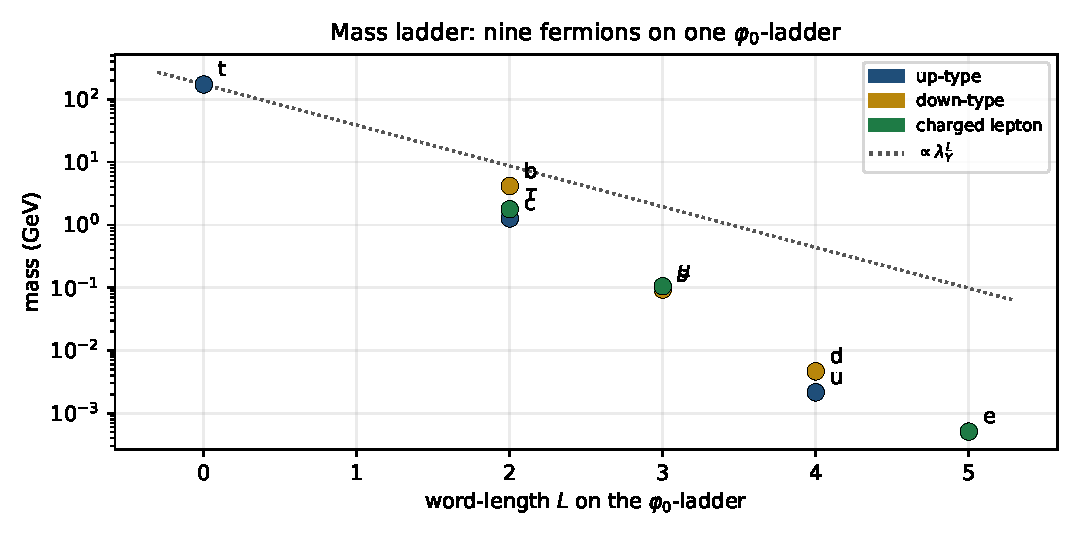
\includegraphics[width=0.86\linewidth]{figures/mass_ladder.pdf}
\caption{Mass ladder (data plot, \texttt{verification/make\_figures.py}). The nine charged fermions
(PDG masses) plotted against their word-length $L$ on the $\phiz$-ladder, coloured by sector; the dotted
line is the geometric reference $\propto\lambda_Y^{L}$ with $\lambda_Y=\sqrt{\phiz(1-\phiz)}$. The whole
five-order hierarchy is one ladder.}
\label{fig:massladder}
\end{figure}

% =====================================================================
\section{The Sheet Diamond and the Winding Line: masses and transport from one surface}
% =====================================================================
The mass-power matrix and the transport word-length matrix are \emph{not} two independent machines: they
are the two sheet-readouts of \emph{one} parabolic projection $Q$ acting on the residue matrix $R$. Collect
the $\phiz$-orders $k_{f,j}$ of the nine charged fermions into the \textbf{mass-power matrix}
\begin{equation}
  K=\begin{pmatrix}4&2&0\\4&3&2\\5&3&2\end{pmatrix}\quad(\text{rows }u,d,e),\qquad
  Q:=L-K=\begin{pmatrix}3&1&0\\3&2&0\\3&2&1\end{pmatrix},\qquad
  \Sigma:=\operatorname{diag}(1,-1,-1),
\end{equation}
with $\Sigma$ the \emph{sheet} ($\Z_2$) involution. Then, exactly,
\begin{equation}
  \boxed{\ K=R+Q\,\Sigma,\qquad L=R+Q\,(I+\Sigma)\ }\qquad\mE\ \veri{v10\_projection\_involution.py} ,
\end{equation}
and since $I+\Sigma=\operatorname{diag}(2,0,0)$ and $Q$'s first column is $(3,3,3)^\top$, the
``hand-added'' first-generation winding is \emph{forced}: $Q(I+\Sigma)=6W=2\Nfam\cdot\mathbf 1e_1^\top$, i.e.\
sheet ($\Z_2$) $\times$ families ($\Z_3$) $=$ the $C_6$ transport. So the $\phiz$-mass powers are the
$\Sigma$-odd readout, and the transport lengths are the $(I{+}\Sigma)$ readout, of the \emph{same}
projection $Q$ on $R$.

\begin{winbox}[The Sheet Diamond: all four operators are points of \emph{one} surface \mE\ (\veri{v94\_sheet\_diamond.py})]
The whole flavor algebra lives on a single two-parameter operator surface,
\[
\begin{gathered}
  M(s,t)=R+Q\,\operatorname{diag}(s,t,t):\\
  R=M(0,0),\qquad K=M(1,-1),\qquad L=M(2,0),\qquad F:=R{+}Q=M(1,1),
\end{gathered}
\]
with the two global invariants
\[
  \det M(s,t)=3st^2+9st+6s+t^2+5t+8,\qquad
  \det B_{M(s,t)}=6st+12s+3t^2+15t+16 .
\]
The mass-transport pencil $K+xQ$ is the \emph{cut} $(s,t)=(1{+}x,\,x{-}1)$, on which the anchor-block
determinant factorises as $(3x{+}2)(3x{+}5)$ --- the master cover of the operator-pencil sections below
(unique up to M\"obius reparametrisation, \veri{v85\_master\_cover.py}). The
factorisation is \textbf{not generic}: the surface carries its own negative controls --- the diagonal cut
$t{=}s$ gives $9s^2{+}27s{+}16$ with discriminant $153$ (non-square; the \emph{same} control discriminant as
the $R$-direction pencils), and the $R{\to}L$ cut $t{=}0$ is linear (degenerate direction, no cover).
\smallskip\\
\noindent\textbf{Centered normal form (\veri{v95\_centered\_diamond.py}).} The diamond is a \emph{centered
cross}: with the center $C:=M(1,0)=\tfrac{R+L}{2}=\tfrac{K+F}{2}$ and the two axes
$U:=Q\operatorname{diag}(1,0,0)=\Nfam\,\mathbf1e_1^\top$ (winding, rank $1$, spectrum $\{3,0,0\}$) and
$V:=Q\operatorname{diag}(0,1,1)$ (sheet, rank $2$),
\[
  \boxed{\ Q=U+V,\qquad R=C{-}U,\quad L=C{+}U,\quad K=C{-}V,\quad F=C{+}V\ }\qquad\mE ,
\]
so five objects collapse to three, and the winding line below \emph{is} the $U$-axis ($L=R+2U$). The sheet
axis carries exactly the cusp class: $\operatorname{Spec}(V)=\{0,1,2\}=\Nfam\{0,\tfrac13,\tfrac23\}$
(cf.\ $Q_+=3\,\mathrm{cusp}+1$ with $\{1,2,3\}$, \vref{v69}/\vref{v72}). The center is tightly typed:
$\det C=14$, $\operatorname{SNF}(C)=(1,1,14)$, $\sum_{ij}C_{ij}=31=2^{\gcar}{-}1=1{+}h^\vee(E_8)$ (the same
$31$ as the IR gap-bound numerator $\|V_{\mathrm{metric}}\|\le31/(8\pi^2)$), $\det B_C=28=2\cdot14$,
$\operatorname{Pl}(C)=(0,14,14)$ and $\operatorname{Pl}_R(C)=7\,(2,3,1)$ --- the same ray $(2,3,1)$ as
$\operatorname{Pl}_R(L)=10\,(2,3,1)$, scalaron-$7$ vs decuple-$10$ scaling. \emph{Typing:} the normal form
and all integers are exact \mE; the ``$G_2$ center'' reading ($14=\dim G_2$, also the constant term of
$\chi_{[K,Q]}=t^3{+}5t{+}14$ and $\sqrt{\sum B_F}$) is an \emph{audit} Lie-dimension match, recorded, not
promoted.
\smallskip\\
\noindent\textbf{Axis curvature and two ladders (\veri{v218\_diamond\_axis\_geometry.py}).} The cross has a
\emph{discrete differential geometry}: the determinant is \emph{linear} along the winding axis and
\emph{quadratic} along the sheet axis,
\[
  \det(C{+}xU)=14+6x,\qquad \det(C{+}yV)=14+14y+4y^2,\qquad \det B_{C+xU}=2\det(C{+}xU),
\]
so winding flows flat ($A_3$-driven, slope $6=|R^+(A_3)|$) while the sheet split \emph{curves} with second
differences $8=\operatorname{rank}E_8$ (determinant) and $6=|R^+(A_3)|$ (anchor block) --- the two curvatures
are exactly the triply-forced $8$ and the $A_3$ positive roots. Two exact ladders ride the same sheet axis.
The \textbf{Pl\"ucker transfer ladder} $\operatorname{Pl}(K)=({-}1,6,4)\to\operatorname{Pl}(C)=(0,14,14)\to
\operatorname{Pl}(F)=(1,22,30)$ lifts in steps $(1,8,10)=(N_\Phi,\operatorname{rank}E_8,A_\Lambda)$ then
$(1,8,16)=(N_\Phi,\operatorname{rank}E_8,\dim S^+)$ --- first the decuple, then the full spinor generation, so
the $F_{\mathrm{transfer}}$ source$\to$pole step \emph{is} this two-stage sheet lift \mC. The \textbf{spectral
ramification ladder} factors the cubic discriminant of $Q,K,C,F$ as $q(r)^2\operatorname{Disc}(q)$ with squares
$(1,3,4,6)=(N_\Phi,\Nfam,|\mu_4|,|R^+(A_3)|)$ and kernels $(13,48,65,105)=(\Delta_Q,\Omega_{\mathrm{adm}},
\gcar\Delta_Q,\Nfam\gcar\cdot7)$, the corner $F$ carrying $105=3{\cdot}5{\cdot}7$ (family $\cdot$ carrier
$\cdot$ scalaron). \emph{Audit:} the anchor-defect spectrum $\Delta_a(Q,K,R,C,L,F)=(8,16,18,21,24,26)$ and the
corner-determinant pair-sum atlas (total $64=\dim S^+|\mu_4|$, staircase sum $81=\Nfam^4$) are recorded
fingerprints --- the $2\dim G_2$ and $\dim F_4$ pair sums stay audit-only, like the $G_2$ center above.
\smallskip\\
\noindent\textbf{$F_{\mathrm{transfer}}$ is a path, not four interfaces (\veri{v224\_diamond\_ftransfer\_path.py}).}
The corners $K{=}M(1,{-}1)$, $C{=}M(1,0)$, $F{=}M(1,1)$ lie on the \emph{sheet axis} $s{=}1$: the determinant
there is the curved $\det M(1,t)=4t^2{+}14t{+}14$ (values $(4,14,32)$, 2nd difference $8{=}\operatorname{rank}E_8$),
while the winding axis $\det M(s,0)=6s{+}8$ is flat. So $F_{\mathrm{transfer}}$ is read as \emph{one discrete
geodesic} $K\to C\to F$ on the diamond (the Pl\"ucker steps $(1,8,10),(1,8,16)$ above), of which the Koide
source$\to$pole M\"obius relaxation is the $1$-D projection (\vref{v37}/\vref{v183}); the external QFT solver
evaluates continuously \emph{along} this known path \mC. The diagonal cut $t{=}s$ mixes the axes (negative
control), so only the $s{=}1$ sheet axis is the branch-preserving transfer direction.
\smallskip\\
\noindent\textbf{The center collects the three local norms (\veri{v230\_center\_budget\_norms.py}).} The
center's row sums are $(7,11,13)$, and these are the three \emph{local norms} of the theory:
$7=N_{\mathbb Z[\omega]}(3{+}2\omega)$ (the Eisenstein/hexagonal CM norm $=$ scalaron exponent),
$13=N_{\mathbb Z[i]}(3{+}2i)$ (the Gaussian/square CM norm $=\Delta_Q$), and
$11=\binom40{+}\binom41{+}\binom42=1{+}4{+}6$ (the QBL boundary Fock count on the four $\mu_4$ corners
$=\dim S^+{-}\gcar=16{-}5$). So $C=(\text{hex norm},\,\text{boundary Fock count},\,\text{square norm})$: the
two exceptional CM rings (\veri{v222\_cm\_norm\_duality.py}) and the seam boundary count meet in one operator
center, the ring assignment rigid \mE.
\smallskip\\
\noindent\textbf{The Winding Line.} On $R_s=R+s\,\mathbf 1e_1^\top$ (the $R\to L$ channel) anchor area and
torsion volume run \emph{synchronously} for all $s$:
\[
  \boxed{\ \det R_s=8+2s,\qquad \det B_{R_s}=16+4s=2\det R_s\ },
\]
and the physical winding $s=6=|R^+(A_3)|$ is fixed by \emph{each} of three closure conditions alone:
$\operatorname{tr}R_s=15=\dim A_3$, $\det R_s=20=\det L$, and the Coxeter lift $(R_s^\top a)_1=30=h(E_8)$.
The mechanism is the \textbf{cofactor seam normal} $n=c_2{\times}c_3=(5,-9,6)$ (cross product of the
second and third \emph{columns} of $R$) --- the common first adjugate row of $R$ \emph{and} $L$ (columns
$2,3$ are winding-invariant) --- with
\[
  n\cdot\mathbf 1=2=|\Z_2|\ (\text{per-winding det increment}),\quad
  n^\top R=(8,0,0),\quad n^\top L=(20,0,0):
\]
the normal annihilates the stable columns, so \emph{generation one is the only open torsion channel} ---
the $+6$ winding is not sorted by hand. \emph{Honest scope:} the winding line crosses the spectral
\emph{reality} threshold at $s^*\!\approx\!2.83$ (not at $6$), so reality is a \emph{property} of the
physical point --- $\operatorname{disc}\chi_L=39200=2(10\cdot14)^2$, spectrum real positive --- not its
selector; and the corner $F=R{+}Q$ is an \emph{audit} operator (the $F_4{\times}G_2$ shadow:
$\det B_F=52=\dim F_4$, $\sum B_F=196=(\dim G_2)^2$), not a physical transport.
\smallskip\\
\noindent\textbf{The dual anchor (\veri{v134\_dual\_anchor.py}).} The anchor's \emph{inverse} response is the
same on both ends of the winding line, and it is the Nariai root of the horizon paper:
\[
  \boxed{\ d:=a^\top R^{-1}=a^\top L^{-1}=\bigl(-\tfrac12,-\tfrac12,1\bigr)\ },\qquad
  d\cdot\mathbf 1=0,\quad d\cdot a=1,\quad (1,1,-2)=-2d .
\]
The invariance is structural (Sherman--Morrison): $L=R+6\,\mathbf 1e_1^\top$ makes a covector
winding-invariant iff it kills $R^{-1}\mathbf 1=\tfrac14(1,1,-1)$; the anchor does, while $\mathbf 1$,
$e_1$ and $n$ do not ($\tfrac14,\tfrac14,-\tfrac52$ --- the membership is special). $(d,n)$ is the dual
normal pair of the flavor boundary: $d$ the \emph{sheet} normal (kills $\mathbf 1$, dual to $a$,
$\propto$ Nariai), $n$ the \emph{torsion} normal (first-generation channel). \mE; bridge reading \mC.
\smallskip\\
\noindent\textbf{Walls of the surface (\veri{v135\_det\_surface.py}).} The surface determinant factorises,
\[
  \boxed{\ \det M(s,t)=3s(t{+}1)(t{+}2)+t^2+5t+8\ },
\]
exposing two \emph{iso-volume walls independent of $s$}: $t=-2\Rightarrow\det=2=|\Z_2|$ and
$t=-1\Rightarrow\det=4=|\mu_4|$ --- so $\det K=4$ is a whole \emph{layer} of the surface ($K=M(1,-1)$ lies
on the $\mu_4$ wall), not an isolated hit --- while the winding line $t=0$ carries $\det=6s+8$, i.e.\
$(\det R,\det C,\det L)=(8,14,20)$, and the fourth corner closes the pattern with
$\det F=\det M(1,1)=32=2^{\gcar}$. The anchor block obeys $\det B_{M(s,0)}=2\det M(s,0)$ \emph{exactly} on
the winding line and has its own $\Z_2$ wall, $\det B_{M(s,-2)}=-2$ ($t=-1$ is \emph{not} a $B$-wall:
$6s+4$, recorded honestly). Row-budget axes: $\operatorname{rowsum}(C)=(7,11,13)$,
$\operatorname{rowsum}(U)=(3,3,3)$ (democratic winding), $\operatorname{rowsum}(V)=(1,2,3)=
\operatorname{Spec}(Q_+)$ verbatim; the centre budget $(7,11,13)=(\text{scalaron},\|\operatorname{Pl}(K)\|_1,
\Delta_Q)$ is an audit match. Two anchor micro-identities: $e_1^2+e_2^2=41=10\,b_1$ (the anchor Pythagoras
for the abelian coefficient, companion to $\Delta_Y=25=9{+}16$) and $p_1^2+p_2^2=52=$ the carrier coset
root count ($40{+}12$, \veri{v128\_graded\_hull.py}). All \mE; the ``2d surface with atom walls'' reading \mC.
\end{winbox}

\begin{keybox}[The $Q_+$ grading is cohomology: one spectrum in four readouts \mE\ (\veri{v137\_qplus\_cohomology.py})]
The sheet axis is not just numerology on $V$: it is the cohomology of the seam curve.
$b_1(\PP\setminus\mu_4)=3=\Nfam$, with holomorphic basis $\omega_k=z^{k-1}dz/(z^4-1)$, $k=1,2,3$
(regular at infinity; the trivial character is absent), and under the $\mu_4$ deck $z\mapsto iz$
\[
  \omega_k\ \longmapsto\ i^k\,\omega_k,\qquad
  \operatorname{res}_{\zeta}\omega_k=\tfrac{\zeta^k}4 :
\]
$H^1=\chi_1\oplus\chi_2\oplus\chi_3$ --- each nontrivial $\mu_4$ character exactly once, and the residue
vector over the punctures \emph{is} the character vector. The character degrees $(1,2,3)$ are exactly
$\operatorname{Spec}(Q_+)$ ($Q_+=3\,\mathrm{cusp}+1$, \vref{v69}/\vref{v72}), and the cusp weights $\{0,\tfrac13,
\tfrac23\}$ underneath are $\operatorname{spec}(A_0^\star)$ (\vref{v115}):
\[
  \boxed{\ \text{MS weights}\ =\ \text{cusp classes}\ =\ H^1\text{ characters}\ =\
  \operatorname{Spec}(Q_+)-1\ \text{over } \Nfam\ }
\]
--- one spectrum in four readouts; and $(1,2,3)$ are the \emph{exponents of $A_3$} ($W(A_3)=S_4$, \vref{v117};
$h(A_3)=4=|\mu_4|$): the $Q_+$ generation grading \emph{is} the $A_3$ exponent grading, realised on the
seam curve's cohomology. \emph{Typing:} all spectrum statements \mE; what remains of \texttt{GATE.QGEO}
is the \emph{naturality} of the identification --- the canonical map from the $H^1$ character basis to
the $V$-axis generation basis ($\operatorname{rowsum}(V)=(1,2,3)$ verbatim, \veri{v135\_det\_surface.py})
--- typed \mC.
\smallskip\\
\noindent\textbf{The canonical map exists and is rigid (\veri{v140\_canonical\_map.py}).} The naturality
residue collapses. Of the established $\mu_4$ actions on generation space, the plain deck
$U=\operatorname{diag}(1,i,-i)$ has characters $(0,1,3)$ --- an invariant line, missing $2$ --- and
\emph{cannot} match $H^1$; but the \textbf{sheet-twisted} deck $-U$ (characters $(2,3,1)$) and the cusp
exponential $i^{Q_+}$ (characters $(1,2,3)$) both carry the character \emph{set} $\{1,2,3\}$ --- exactly
the $H^1$ set, by the same sign twist that builds the \vref{v118} hexagon. Both sides are multiplicity-free, so
by Schur the equivariant isomorphism \emph{exists and is unique} up to one scalar per character: the
canonical map is well-defined --- existence and uniqueness are no longer open. Under the $i^{Q_+}$-map
the $H^1$ Euler degree pulls back to $Q_+$ itself; under the $-U$-map to $Q_+\!\circ\rho$ with $\rho$ the
$(123)$ family rotation: the two candidates differ by \emph{exactly one} $\Z_3$ rotation. \emph{Typing:}
character algebra, rigidity and grading transport \mE.
\smallskip\\
\noindent\textbf{The deck selection theorem: the $\Z_3$ choice is \emph{derived}
(\veri{v141\_deck\_selection.py}).} The discrete choice does not survive contact with the integer model
the suite already owns: the derived integer deck $G=T_A\Sigma$ (\veri{v97\_sheet\_conjugation\_bridge.py}/%
\veri{v98\_discriminant\_dictionary.py}) has the $Q_+{=}1$ cusp line as an \emph{exact} eigenline with
eigenvalue $-1=i^2$ --- the self-conjugate character $2$ --- and the conjugate pair $\{1,3\}$ on the
$E$-plane. Of the three $\Z_3$ rotations only the sheet-twisted assignment $(2,3,1)=\mathrm{chars}(-U)$
puts character $2$ on the $Q_+{=}1$ line: \textbf{the geometric boundary deck is the sheet-twisted class;
the cusp exponential $i^{Q_+}$ is excluded} (same eigenvalue multiset $\{-1,\pm i\}$, wrong grading
pairing --- the $(-1)$-eigenlines sit on $Q_+$ degrees $1$ vs $2$). An explicit $Q_+{=}1$-line-preserving
conjugacy $SGS^{-1}=-U$ exists; under the relabeling $k\to-k$ only the plane orientation flips $=$ the
established sheet $\Z_2$ (the two Lagrangian glues, \vref{v92}) --- no new residual. Consequence: the
$H^1$ Euler degree pulls back to $Q_+\!\circ\rho$; cusp grading and Euler grading differ on generation
space by exactly the one family rotation $\rho=$ the $\operatorname{coker}Q$ triality (\vref{v72}).
\emph{Typing:} selection, conjugacy and obstruction \mE\ (lattice-level theorem); what remains of
\texttt{GATE.QGEO} is only the realisation premise the gate always carried (the integer $D_4$ model
\emph{is} the parabolic geometry, \vref{v69}/\vref{v98}) \mC\ --- with \emph{no} discrete freedom left.
\smallskip\\
\noindent\textbf{The M\"obius $D_4$ realisation: the premise at its floor
(\veri{v146\_moebius\_d4.py}).} The realisation premise itself now has every checkable part checked.
The \emph{full} dihedral symmetry group of the seam curve, $\langle\delta\!:z\mapsto iz,\ \iota\!:z\mapsto
1/z\rangle=D_4$, acts on the explicit cohomology basis $\omega_k=z^{k-1}dz/(z^4{-}1)$ exactly as the
integer model: $\delta^*\omega_k=i^k\omega_k$ (the deck, \vref{v137}), and
\[
  \boxed{\ \iota^*\omega_1=\omega_3,\quad \iota^*\omega_2=\omega_2,\quad \iota^*\omega_3=\omega_1\ }
\]
--- the exponent duality with parity $+1$ on the self-conjugate line and $\det=-1$, \emph{no extra
phases}. In the cusp basis the anchor-forced conjugation $T_A$ \emph{is} this permutation (fixes the
character-$2$ line with $+1$, $\det=-1$ $=$ the glue-swap parity), and $\Sigma$ \emph{is} the
$\delta\iota$ class ($-1$ on the character-$2$ line, $\det=+1$ $=$ glue-fix): the \vref{v98}
reflection-class split lands exactly on the geometric reflection classes. \emph{Typing:} the dihedral
match \mE; with spectra (\vref{v137}), cyclic part (\vref{v141}) and reflections now all matched, the
premise reduces to the module identification itself --- ``generation space \emph{is} $H^1$ of the seam
curve with its parabolic weights'' \mC\ --- with no remaining checkable mismatch.
\end{keybox}

\begin{winbox}[Spectra and the determinant ladder $\to|W(D_5)|$ \mE]
The two operators carry the compiler atoms in their characteristic polynomials,
\begin{equation}
  \chi_Q=(t-1)(t^2-5t+3)\ \ [\,\gcar,\Nfam\,],\qquad
  \chi_K=(t-1)(t^2-8t+4)\ \ [\,h(D_5),|\mu_4|\,],
\end{equation}
with discriminants $\Delta_Q=13=|R(A_3)|{+}1$ and $\Delta_K=48=\Oadm$. Their determinants form a torsion
ladder ($\operatorname{coker}=\Z_3,\Z_4,\Z_8,\Z_{20}$),
\begin{equation}
\begin{gathered}
  (\det Q,\det K,\det R,\det L)=(3,4,8,20),\\[2pt]
  \boxed{\ \det Q\cdot\det K\cdot\det R\cdot\det L=1920=|W(D_5)|\ }\qquad\mE ,
\end{gathered}
\end{equation}
tying flavor residues, mass powers, transport and the $D_5$ Weyl group (the same $1920$ that appears in the
horizon Hawking-power denominator). The sheet decomposition is sharp: $\operatorname{Spec}(Q_+)=\{1,2,3\}$
are the $A_3$ exponents ($\det Q_+=6=|R^+(A_3)|$), $\chi_{Q_-}=t(t^2-3)$ (a square root of $\Nfam$), and
$\chi_{K_-}=t(t^2-8)$ (a square root of $h(D_5)$). Finally the EM budget sits in the $K$ anchor block:
$a^\top K a=41=10b_1$ with $a=(1,1,2)$, and $\det\!\begin{psmallmatrix}\mathbf1^\top K\mathbf1&\mathbf1^\top Ka\\ a^\top K\mathbf1&a^\top Ka\end{psmallmatrix}=\det\begin{psmallmatrix}25&29\\35&41\end{psmallmatrix}=10=\AL$.
\veri{v10\_projection\_involution.py}, \veri{v12\_mass\_generation\_polynomials.py}
\smallskip\\
\noindent\textbf{Mass volume and the EM budget are \emph{one} anchor operation
(\veri{v74\_compiler\_micro\_lemmas.py}).} The two diagonal entries of $B_K$ are the two physical readouts:
$\mathbf1^\top K\mathbf1=25=\gcar^2$ is the grand \emph{mass-volume} exponent ($\det M_{\rm SM}\!\sim\!(\phiz)^{25}$),
and $a^\top K a=41=10b_1$ is the \emph{EM budget}. Their difference is one generation,
\[
  \boxed{\ a^\top K a-\mathbf1^\top K\mathbf1=41-25=16=\dim S^+\ },
\]
i.e.\ \emph{EM budget $=$ mass volume $+$ one generation}. So the number $41$ that the EM fixed point reads is
not ``$40{+}1$'' but the anchor quadratic form of the mass-power matrix, tied to the mass volume $\gcar^2$ by
a single half-spinor $\dim S^+$.
\end{winbox}

\begin{winbox}[Mass and transport are one pencil: $\det(K+xQ)$ carries the scalaron sequence \mE]
Because $L=K+Q$, the mass-power matrix $K$ and the transport matrix $L$ are the two endpoints
($x=0,1$) of a \emph{single} one-parameter compiler pencil $P(x)=K+xQ$, whose determinant is
\[
  \boxed{\ \det(K+xQ)=3x^3+7x^2+6x+4\ },\qquad
  (3,7,6,4)=\bigl(\Nfam,\ \Oadm-10b_1,\ |R^+(A_3)|,\ |\mu_4|\bigr),
\]
i.e.\ the coefficient sequence is $N_{\mathrm{fam}}$, the \emph{scalaron exponent} $7$, the $A_3$ positive
roots and the glue index --- one curve linking flavor, the Starobinsky scalaron, the family and the glue.
The pencil is anchored at four integer nodes by compiler atoms:
$P(-1)=2=|\Z_2|$ (the $K{-}Q$ sheet endpoint, with $\det(K{-}Q)=|\Z_2|$, $\operatorname{tr}(K{-}Q)=\Nfam$),
$P(0)=4=\det K=|\mu_4|$, $P(1)=20=\det L$, and $P(2)=68=2\,p_5(a)$ (twice the anchor power sum $p_5=34$).
\veri{v52\_pencil\_endpoints.py}
\smallskip\\
\noindent\textbf{And the consecutive \emph{differences} are the sheet$\to$matter chain
(\veri{v74\_compiler\_micro\_lemmas.py}).} The node values $(2,4,20,68)$ step by
\[
  \boxed{\ P(0){-}P(-1)=2=|\Z_2|,\quad P(1){-}P(0)=16=\dim S^+,\quad P(2){-}P(1)=48=\Oadm\ }
\]
i.e.\ $2\to16\to48$ --- \emph{sheet $\to$ one generation $\to$ three generations} --- so the single
determinant pencil already encodes the passage from the $\Z_2$ sheet to the one-family half-spinor to the
full admissible matter packet. The $(K,Q,L)$ operators are therefore not separate artefacts but one curve.
The non-commutativity of the mass$\to$transport step is a fixed $G_2$-sized obstruction:
$[K,L]=[L,Q]=[K,Q]$ (forced by $L=K+Q$) with $\chi_{[K,Q]}(t)=t^3+5t+14$, reading $\gcar=5$ and
$\dim G_2=14$ (audit-level \mO). \veri{v37\_plucker\_anchor.py}
\end{winbox}

\begin{keybox}[Operator-pencil geometry: the anchor plane as a small area in operator space \mE\ (\veri{v80\_operator\_pencil\_geometry.py})]
Read the four operators through the \emph{anchor block} $B_M=\begin{psmallmatrix}\mathbf1^\top M\mathbf1&\mathbf1^\top Ma\\a^\top M\mathbf1&a^\top Ma\end{psmallmatrix}$.
\textbf{(i) Anchor Singularity Theorem.} On the pencil $P(x)=K+xQ$,
\[
  \boxed{\ \det B_{K+xQ}=9x^2+21x+10=(\Nfam x+|\Z_2|)(\Nfam x+\gcar)=(3x+2)(3x+5)\ }\qquad\mE ,
\]
so the oriented anchor area \emph{degenerates} at exactly $x=-|\Z_2|/\Nfam=-\tfrac23$ and $x=-\gcar/\Nfam=-\tfrac53$.
The first zero is the Koide target / transport-gap base ($\lambda_2=(\tfrac23)^6$); the second is the $D_5/A_3$
glue asymmetry. \textbf{So $\tfrac23$ is not just a recurring fraction --- it is the first singular point of the
mass$\leftrightarrow$transport anchor plane}, a structural \emph{location} where an oriented area collapses.
\textbf{(ii) Type checker.} The anchor-block determinants classify the operators:
$\det B_Q=9=\Nfam^2$ (family square), $\det B_K=10=\AL$ (pair sector), $\det B_R=16=\dim S^+$ (one generation),
$\det B_L=40=|R(D_5)|$ (carrier root budget) --- each a determinant of a fixed block, not a loose integer.
\textbf{(iii) Buildup chain.} The pencil coefficients $(3,7,6,4)$ have partial sums $(3,10,16,20)=(\Nfam,\AL,\dim S^+,\det L)$,
so the scalaron exponent is the internal flavor transition $7=\AL-\Nfam$.
\smallskip\\
\noindent\emph{Audit layer (exact values \mE, decorative reading \mC).} $D(x)=\det(K{+}xQ)$ and its derivatives
at $x=-1,0,1,2$ give $(2,4,20,68),(1,6,29,70),(-4,14,32,50)$ ($29$ the top $E_8$ exponent, $32=2^{\gcar}$, $50$
the $A_4{\times}A_4$ off-block); and the missing corner $F=R+Q$ has $\det B_F=52=\dim F_4$ with
$248=52+14+26\cdot7$ --- the genuine $E_8\!\supset\!F_4{\times}G_2$ branching $(52,1){\oplus}(1,14){\oplus}(26,7)$
as an operator \emph{shadow}. These are exact identities; their atlas/embedding significance is kept audit-level
(\mC), since the coefficients are themselves atoms.
\end{keybox}

\begin{keybox}[The Koide point is one branch of a double cover \mE\ (\veri{v81\_singular\_pencil\_matrices.py})]
The anchor-block determinant $\det B_{K+xQ}=(3x+2)(3x+5)$ is \emph{quadratic}, so
\[
  \boxed{\ y^2=\det B_{K+xQ}=(3x+2)(3x+5)\ }
\]
is a $2{:}1$ cover of the pencil line, \emph{ramified exactly over its two zeros}. Hence the Koide/gap point
$x=-|\Z_2|/\Nfam=-\tfrac23$ and the carrier point $x=-\gcar/\Nfam=-\tfrac53$ are \textbf{the two branch points of
one double cover}: \emph{Koide is literally ``the other side'' of the carrier point}. The deck involution is
$y\mapsto-y$ of degree $2=|\Z_2|$ --- the sheet itself --- which is the line-bundle reflection of the
$\mathrm{Spin}(10)\!\to\!\mathrm{SO}(10)$ half-spinor cover the carrier lives on. Three rigid readings:
\begin{itemize}\setlength\itemsep{1pt}
  \item \textbf{Branch locus $=$ spine ends / family.} The ramification is at $-2/3$ and $-5/3$, i.e.\
  $-(|\Z_2|,\gcar)/\Nfam$ --- the \emph{two ends} of the spine $(2,3,4,5)$ over $\Nfam$.
  \item \textbf{Discriminant $=\Nfam^4=81$} (a perfect square $\Rightarrow$ rational, split branch points);
  $\sqrt{81}=9=\Nfam^2=\det B_Q$.
  \item \textbf{Separation $=1=$ one transport period} (the $K\!\to\!L$ step $x:0\!\to\!1$); the deck-translation
  $x\mapsto x+1$ carries the carrier point onto the Koide point.
  \item \textbf{Branch divisor $=$ (scalaron, $\AL$).} Sum of branch points $=-7/3=-7/\Nfam$, product $=10/9=\AL/\Nfam^2$;
  the integer labels $\{|\Z_2|,\gcar\}=\{2,5\}$ have $\mathrm{sum}=7$, $\mathrm{prod}=10=\AL$, $\mathrm{diff}=3=\Nfam$.
  \textbf{So the scalaron is the \emph{trace} of the branch divisor} --- its several readouts ($\Oadm{-}10b_1$,
  $\AL{-}\Nfam$, $\gcar{+}|\Z_2|$, the mixed anchor area) collapse to this one geometric origin.
  \item \textbf{The sheet lives on the cut.} The fibre $y^2{=}\det B$ is $\AL$ at $K$ and $4\AL$ at $L$, so transport
  multiplies $y$ by $|\Z_2|$; the $\Z_2$ sheet endpoint $x{=}{-}1$ sits \emph{between} the branch points where
  $y^2{=}\det B_{K-Q}{=}{-}|\Z_2|{<}0$ --- on the imaginary branch cut joining Koide and the carrier.
\end{itemize}
\noindent At each branch point the pencil clears its $3$-denominator into an integer compiler matrix.
\emph{Koide} $C_{2/3}=3K-2Q$ reproduces the carrier glue: $\operatorname{tr}=15=\dim A_3$, $\textstyle\sum=45=\dim D_5$,
$\det=60=D_{\mathrm{start}}$, and the (now forced rank-one) anchor block
$B_{C_{2/3}}=\begin{psmallmatrix}45&55\\63&77\end{psmallmatrix}=\binom{\gcar}{7}\,(\,\Nfam^2\ \ 11\,)$ with
$\sum=240=|R(E_8)|$. \emph{Carrier} $C_{5/3}=3K-5Q$ is the charge-\emph{neutral} side ($\sum_{ij}=0$) with
$\chi(\lambda)=(\lambda+|\Z_2|)(\lambda^2+\lambda+|R^+(A_3)|)=(\lambda+2)(\lambda^2+\lambda+6)$, splitting off
the sheet eigenvalue $-|\Z_2|$. So the recurring $\tfrac23$ is not a quotient that ``appears everywhere'' --- it
is one ramification point of the mass$\leftrightarrow$transport double cover. The sharper open question is then
\emph{why the leptonic source-to-pole transfer renormalises onto a branch point, and which sheet ($y\to\pm$) the
parity selects} --- a cleaner target than ``why $2/3$''. (The $D_5/A_3$ and $E_8$ labels on the clearing matrices
are exact; their per-entry atlas reading stays audit-level \mC.) \emph{Gravitational twin:} the same split
$\Nfam$-linear double-cover structure reappears in classical gravity --- the Schwarzschild--de~Sitter mass
line has $\operatorname{disc}\propto(1-3m)(1+3m)$ (branch points $\pm1/\Nfam$, separation $2/3$, deck $=$
horizon swap), the Nariai roots are the traceless anchor $(1,1,-2)$, and $2/3$ is the exact Nariai/de-Sitter
entropy bound (Appendix~H; \veri{v101\_horizon\_anchor.py}).
\end{keybox}

\begin{keybox}[The Koide branch is a \emph{forced} attractor, and the clean split is non-generic \mE/\mC\ (\veri{v82\_koide\_attractor\_splitting.py})]
This sharpens the open question above. Work in the branch coordinate $q=-3x$ (Koide $q=2$, carrier $q=5$).
\textbf{(A) The source-to-pole map is forced, not postulated.} Any branch-divisor-preserving M\"obius map of the
pencil line that fixes \emph{both} branch points is, in the cross-ratio coordinate $\rho=(q-2)/(5-q)$, exactly
$\rho\mapsto\mu\rho$ --- hence \emph{unique} once $\mu$ is fixed. The multiplier is not a new input: $\mu=(2/3)^6$
is the subleading eigenvalue $\lambda_2$ of the \emph{already-established} unique gapped boundary transfer operator
(spectrum $\{1,(2/3)^6,(1/3)^6\}$, gap $6\log\tfrac32>0$; \veri{v54\_seam\_horizon\_keystones.py}, \veri{v56\_unique\_attractor.py}),
and the Koide branch $x=-2/3=-|\Z_2|/\Nfam$ is precisely its cusp weight $2/3=\{0,1,|\Z_2|\}/\Nfam$ (the carrier maps to
Koide under the deck period $q\mapsto q-\Nfam$, the same cusp class). With $\mu=(2/3)^6$ the unique map is the integer
M\"obius map
\[
  \boxed{\ F(q)=\frac{2(569q-3325)}{665q-3517}\ },\qquad F(2)=2,\ \ F(5)=5,\ \ F'(2)=(2/3)^6<1,\ \ F'(5)=(3/2)^6>1,
\]
so Koide is the \textbf{attractor} and the carrier the \textbf{repeller}, and $q_n\to2$ i.e.\ $x\to-2/3$ at the
\emph{same} rate that governs the SM flavor gap and horizon recovery. The three structural postulates needed for a
Koide derivation thus collapse to \emph{one} physical identification --- \emph{source-to-pole transfer $=$
branch-preserving relaxation of the established transfer operator} --- after which rate, uniqueness and direction
all follow. That single identification stays \mC; the rest is \mE. \textbf{(B) The clean rational split is
non-generic.} The splitting-type exponents $(2,1,1)$ (the anchor $a=(1,1,2)$) placed across the three family slots
give three different covers: $(1,1,2)$ gives $\det B_{K+xQ}=(3x+2)(3x+5)$, $\mathrm{disc}=81=\Nfam^4$ (\emph{split},
rational labels $\{2,5\}$); $(2,1,1)$ gives $(x+2)(9x+11)$, $\mathrm{disc}=49=7^2$ (\emph{split}); $(1,2,1)$ gives
$5x^2+10x+3$, $\mathrm{disc}=40=|R(D_5)|=\det B_L$, which is \emph{not} a square --- a \textbf{non-split} cover with
Galois-conjugate branch points $-1\pm\sqrt{10}/5$ centred exactly on the sheet $x=-1$ ($q=3$), separation
$2\sqrt{\AL}$. (Negative control, as for the cover itself: the $R$-pencil has $\mathrm{disc}=153$, also not a
square.) So Koide and the carrier appearing as \emph{separate rational} singularities is a special feature of the
canonical anchor placement, not a generic one --- a hardening of anchor-first. The physical fermion-sector
identification of the three placements is not claimed and stays \mC.
\end{keybox}

\begin{keybox}[Branch kernels select the sectors; one deck involution \mE\ (\veri{v96\_branch\_kernel\_selection.py}, \veri{v97\_sheet\_conjugation\_bridge.py})]
The ``which sheet does parity select'' question above had a blocker: no \emph{independently motivated}
sector$\to$sheet map. The cover supplies one itself. At each branch point the anchor block is \textbf{rank
one}, with canonical \emph{integer} kernels:
\[
\begin{aligned}
  &\text{Koide } x=-\tfrac23:\ \ w=11\,\mathbf1-9a=(2,2,-7),\quad v=7\,\mathbf1-5a=(2,2,-3);\\
  &\text{carrier } x=-\tfrac53:\ \ w=\mathbf 1,\quad v=8\,\mathbf1-7a=(1,1,-6),
\end{aligned}
\]
--- at the carrier point the block annihilates the \emph{democratic vector itself}. \textbf{Collapse lemma
\mE:} rank one forces $P(x_0)\,w\perp\operatorname{span}\{\mathbf1,a\}$, hence proportional to the
antisymmetric direction $(-1,1,0)$ of the anchor's two \emph{equal} slots --- on both sides:
\[
  P(-\tfrac23)\,w=\tfrac{20}{3}\,(1,-1,0),\qquad P(-\tfrac53)\,w=\tfrac23\,(-1,1,0),\qquad
  v^\top P(x_0)\propto(-1,1,0)\ \text{at both points} .
\]
Reading the rows as the sectors $(u,d,e)$: \emph{up and down are the deck-odd pair} ($f_u=-f_d$;
convention-free, $f_uf_d<0$ at both points), and the \emph{lepton pairing vanishes} --- the leptons sit
\emph{on} the ramification, consistent with Koide being a charged-lepton relation. Indeed the lepton
pairing forms \emph{are} the two det-$B$ factors: the \textbf{sector zero ladder} reads
lepton $\to\{-\tfrac23,-\tfrac53\}$ (the branch points), up $\to-\tfrac32=-\Nfam/|\Z_2|$ \emph{doubly}
(the whole up-row of $P(-\tfrac32)$ \emph{is} the odd direction $-\tfrac12(1,-1,0)$ --- the previously
unexplained $\mathrm{GL}(2)$ rung), down $\to\{0\ (=K),\ -\tfrac95=-\Nfam^2/\gcar\}$. The deck translation
flips the orientation $(+,-)\to(-,+)$ with magnitude ratio $10=\AL$. \emph{Controls:} anchor $(2,1,1)$
moves the collapse to $(0,1,-1)$; $(1,2,1)$ is non-split (disc $40$), no rational kernels at all.
\smallskip\\
\noindent\textbf{The bridge to the glue chiralities (\veri{v97\_sheet\_conjugation\_bridge.py}).} The two
$E_8$ glues are swapped by \emph{either single} spinor conjugation and fixed by the simultaneous one
(\veri{v92\_glue\_uniqueness.py}); on the family side, conjugation negates the cusp classes
($0$ fixed, $\tfrac13\leftrightarrow\tfrac23$ on the $Q_+$ eigenspaces $e_1=(0,0,1)$, $e_2=(0,1,2)$,
$e_3=(1,0,0)$). That conjugation has a \emph{unique anchor-compatible} integer realisation: $T\mathbf1=\mathbf1$
and $Ta=a$ \emph{both} force the same scale, giving
\[
  \boxed{\ T_A=\begin{psmallmatrix}0&1&0\\1&0&0\\2&-2&1\end{psmallmatrix},\quad T_A^2=I,\quad\det T_A=-1\ },
  \qquad\text{and}\qquad \boxed{\ a=e_2+e_3\ }
\]
--- \emph{the anchor is the conjugation-symmetrised vector of the swapped pair} (the two alternative
pairings admit \emph{no} anchor-compatible scale). On the quotient by the anchor plane, $T_A=-1$ exactly
like the sector transposition: \textbf{one deck action where the cover lives}. The parity matches the glue
arithmetic ($\det=-1$ single/swapping vs $\det\Sigma=+1$ simultaneous/fixing); $\langle T_A,\Sigma\rangle$
closes the \emph{same} $D_4=\Z_4\rtimes\Z_2$ as the $Q$-geometry, with $\chi_{T_A\Sigma}=(t{+}1)(t^2{+}1)$
identical to the $\mu_4$ homology matrix; and the \textbf{sheet-index lemma}: the generation-$\mu_4$ and the
homology-$\mu_4$ are rationally but \emph{not} $\mathrm{GL}(3,\Z)$-conjugate --- every intertwiner has
\emph{even} determinant, minimum $|\det|=2=|\Z_2|$ (one sheet doubling; independent of $\det Q=\Nfam$).
\smallskip\\
\noindent\textbf{The dictionary is derived, not assumed (\veri{v98\_discriminant\_dictionary.py}).}
The generation space carries an \emph{integer} $\mu_4$: $G:=T_A\Sigma$ acts on the cusp basis as
\[
  \boxed{\ G\,e_1=-e_1,\qquad G\,e_3=e_2,\qquad G\,e_2=-e_3\ }\qquad
  (G^4=I,\ \ \chi_G=(t{+}1)(t^2{+}1)),
\]
i.e.\ the $B_1\!\oplus\!E$ decomposition of the $D_4$-equivariant $Q$-geometry realised \emph{integrally}:
$e_1$ spans the $B_1$ line ($G$-eigenvalue $-1$ $=$ the self-conjugate $\Z_4$ class $2$), and
$\operatorname{span}\{e_2,e_3\}$ is the $E$-plane (eigenvalues $\pm i$ $=$ the conjugate class pair
$\{1,3\}$). \textbf{So the cusp-$0$ line \emph{is} the self-conjugate discriminant line, and the swapped
cusp pair \emph{is} the conjugate class pair} --- the dictionary \emph{``$Q_+$ grading $=$ $A_3$
discriminant grading''} holds inside the model. Consistently: $T_A G T_A^{-1}=G^{-1}$ (the discriminant
conjugation $k\mapsto-k$), $q_{A_3}(1)=q_{A_3}(3)=\tfrac38$ (equal on the swapped pair) with
$q_{A_3}(2)=\tfrac12$ fixed, and the two $D_4$ reflection classes separate exactly the glue arithmetic:
$T_Ae_1=+e_1$, $\det=-1$ (glue-\emph{swapping}) vs $\Sigma e_1=-e_1$, $\det=+1$ (glue-\emph{fixing}),
with $\Sigma=T_AG$. \emph{Honest scope:} the sheet question therefore carries \textbf{no separate \mC\
residual any more} --- what remains is exactly the already-open $Q$-geometry realisation gate
(\textsc{gate.qgeo}, the parabolic construction that realises the documented $Q$ on
$\PP^1\!\setminus\!\mu_4$); conditional on that established typing, the sector$\to$sheet selection is
\emph{closed}: up/down are the deck-odd pair, the leptons sit on the ramification, and the deck involution
is the $A_3$-side spinor conjugation realised as $T_A$.
\end{keybox}

\begin{winbox}[Grand Mass Volume: the absolute mass-scaling normalisation \mE]
The individual $c_q$ are a gauge, but the \emph{absolute} normalisation of the mass spectrum is fixed by the
sector mass-matrix \emph{determinants} --- each a clean $\phiz$-power whose exponent is the $K$-row sum:
\[
  \det\!M_{\mathrm{up}}\!\sim\!(\phiz)^{6}\!=\!(\phiz)^{|R^+(A_3)|},\quad
  \det\!M_{\mathrm{down}}\!\sim\!(\phiz)^{9}\!=\!(\phiz)^{\Nfam^2},\quad
  \det\!M_{\mathrm{lep}}\!\sim\!(\phiz)^{10}\!=\!(\phiz)^{\AL},
\]
\[
  \boxed{\ \det M_{\mathrm{SM}}\sim(\phiz)^{6+9+10}=(\phiz)^{25}=(\phiz)^{\gcar^2}=(\phiz)^{\Delta_Y}\ }
\]
the \emph{Grand Mass Volume}. The $Q$-row sums $(4,5,6)=(|\mu_4|,\gcar,|R^+(A_3)|)$ total $15=\dim A_3$, and
$25+15=40=\sum L=|R(D_5)|$ (mass volume $+$ shift volume $=$ transport budget). So the absolute scaling is an
\mE\ determinant identity (each sector $=$ its $K$-row sum); the only genuine scale input is the overall
$v_{\mathrm{geo}}$, not a per-coefficient freedom. \veri{v46\_grand\_mass\_volume.py}
\end{winbox}

\noindent\textbf{Uniqueness (not fitted).} $K$ and $Q$ are the \emph{unique} nonnegative-integer $3\times3$
matrices with their row sums, column sums, characteristic polynomial and per-sector monotone hierarchy ---
verified by exhaustive enumeration \veri{v11\_unique\_KQ.py}. They are forced by small compiler budgets plus
spectrum, not chosen.

\begin{keybox}[Theorem Q --- the $\Sigma$-split as a parabolic projection (sharper uniqueness) \mE/\mC]
The sheet involution $\Sigma=\operatorname{diag}(1,-1,-1)$ splits $Q$ into two parabolic pieces:
\[
  Q_+=\tfrac12(Q+\Sigma Q\Sigma)=\begin{psmallmatrix}3&0&0\\0&2&0\\0&2&1\end{psmallmatrix},\quad
  Q_-=\tfrac12(Q-\Sigma Q\Sigma)=\begin{psmallmatrix}0&1&0\\3&0&0\\3&0&0\end{psmallmatrix},
\]
\[
  \begin{gathered}
  \chi_{Q_+}(t)=(t-1)(t-2)(t-3)\ \Rightarrow\ \operatorname{Spec}(Q_+)=\{1,2,3\}\ (A_3\text{ exponents}),\\[2pt]
  \chi_{Q_-}(t)=t(t^2-3)\ \Rightarrow\ Q_-^2|_{\mathrm{supp}}=3=\Nfam .
  \end{gathered}
\]
\textbf{Uniqueness:} $Q$ is the \emph{unique} nonnegative-integer matrix with $\operatorname{rows}=(4,5,6)$,
$\operatorname{cols}=(9,5,1)$, $\chi_{Q_+}=(t-1)(t-2)(t-3)$ and $\chi_{Q_-}=t(t^2-3)$ (exhaustive
enumeration, \veri{v50\_q\_geometry.py}). So $Q_+$ is the $A_3$ exponent grading, $Q_-$ the $\mu_4$ sheet
coupling, and $K=R+Q\Sigma$ is the \emph{second $\Sigma$-shadow of the same parabolic flavor operator}, not
an imported mass trick.

\smallskip\noindent\textbf{$D_4$-equivariant derivation (\veri{v69\_d4\_q\_geometry.py}) --- gate advanced
\mC/\mE.} The four punctures $\mu_4=\{1,i,-1,-i\}$ are the vertices of a square with symmetry
$D_4=\Z_4\rtimes\Z_2$ (the $90^\circ$ rotation $z\!\mapsto\!iz$ \emph{is} $\mu_4$; the reflection is the
sheet parity $\Sigma$). The $\Z_4$ $4$-cycle on the punctures acts on $H_1(\PP^1\!\setminus\!\mu_4)=\Z^4/(\text{sum}{=}0)=\Z^3$
(the three families) with eigenvalues $\{i,-1,-i\}$, and the $D_4$ permutation rep decomposes as
$A_1\!\oplus\!B_1\!\oplus\!E$, so $H_1=B_1\oplus E$. On this,
\[
  \begin{gathered}
  Q_+=3\,(\text{cusp weights }\{0,\tfrac13,\tfrac23\})+1=\operatorname{diag}(1,2,3),\\[2pt]
  Q_-=\text{$E$-block coupling }\sqrt{\Nfam}\ (B_1\ \text{in the kernel}),
  \end{gathered}
\]
which reproduce $\chi_{Q_+}=(t{-}1)(t{-}2)(t{-}3)$ and $\chi_{Q_-}=t(t^2{-}3)$ exactly. So the $\Sigma$-split
\emph{is} the $D_4=\Z_4\rtimes\Z_2$ structure ($\Z_4{=}\mu_4$ gives the three eigenspaces and $Q_+$; the
$\Z_2$ reflection is $\Sigma$, giving the even/odd split). \textbf{Typing:} the spectra and the
$\Sigma$-split are now \emph{derived} from the $D_4$-equivariant geometry \mE; the residual is only that the
cusp weights $\{0,\tfrac13,\tfrac23\}$ are the established monodromy exponents (\vref{v61}) and the explicit integer
$Q$ still needs the lattice datum --- now \emph{sharpened to a single named invariant}
(\veri{v70\_q\_integer\_lift.py}): in the $\mu_4$-puncture homology basis the $\Z_4$ rotation is the
\emph{unimodular} $R=\begin{psmallmatrix}0&0&-1\\1&0&-1\\0&1&-1\end{psmallmatrix}$ ($\det{=}{-}1$, eigenvalues
$\{-1,i,-i\}$), while the transport has $\boxed{\det Q=3=\Nfam}$ (SNF $\operatorname{diag}(1,1,3)$). So the
integer lift is exactly the parabolic-degree-$0$ embedding carrying the extra $\det=\Nfam$ (the family
multiplicity) that $D_4$ alone (unimodular) does not supply --- one named lattice invariant, no longer a
diffuse ``derive $Q$''.
\smallskip\\
\noindent\textbf{And that invariant is the cusp order itself (\veri{v72\_q\_det\_from\_cusp.py}).} The extra
$\det Q=\Nfam$ is \emph{not} an independent lattice input: $\det Q=|\!\operatorname{coker}Q|=3$ equals the
\emph{order of the cusp monodromy class} (eigenvalues $\{1,\omega,\omega^2\}$, $\omega^3{=}1$) $=$ the common
\emph{denominator} of the very cusp weights $\{0,\tfrac13,\tfrac23\}$ that fix $\operatorname{Spec}(Q_+)$. So
$\det Q=\Nfam$ comes from the \emph{same} cusp datum as the spectrum, and $\operatorname{coker}Q=\Z/\Nfam$ is
the deck group of the degree-$\Nfam$ triality cover defining the family space --- the integer lift is derived
from the geometry, not posited (\mE\ chain; the coker$=$deck-group identification is the standard non-abelian
Hodge reading \mE).
\end{keybox}

\begin{gapbox}[Status: $Q$-geometry derived (spectra, $\Sigma$-split \emph{and} integer lift) \mE]
What is \emph{proved} (\mE): the algebraic identities $K=R+Q\Sigma$, $L=R+Q(I+\Sigma)$, the spectra, the
$1920$ determinant ladder, the anchor block --- all machine-checked. \textbf{Newly advanced (\veri{v69\_d4\_q\_geometry.py}):}
the $D_4$-equivariant origin of the \emph{$Q$-spectra and the $\Sigma$-split} is now derived --- $Q_+$ is the
$3w{+}1$ image of the cusp weights $w\in\{0,\tfrac13,\tfrac23\}$ on the three $\mu_4{=}\Z_4$ eigenspaces of
$H_1(\PP^1\!\setminus\!\mu_4)$, and $Q_-$ is the $E$-block coupling $\sqrt{\Nfam}$ on $H_1=B_1\oplus E$, with
$\Sigma$ the $\Z_2$ reflection of $D_4=\Z_4\rtimes\Z_2$. So the $\phiz$-mass ladder and the transport are two
$\Sigma$-shadows of one $D_4$-equivariant parabolic operator. \textbf{Integer lift closed to the cusp order
(\veri{v72\_q\_det\_from\_cusp.py}):} the one remaining lattice datum $\det Q=\Nfam$ is the order of the cusp
class $=$ the denominator of the same cusp weights, i.e.\ the \emph{same} geometry that fixes the spectrum
(coker$\,Q=\Z/\Nfam=$ triality deck group). So the $Q,\Sigma$ algebra is now an \mE\ layer whose spectra,
$\Sigma$-split \emph{and} integer lift are all read from the order-$\Nfam$ cusp structure; the only standing
input is the established fact $\Nfam=3=\operatorname{rank}A_3=\dim H_1$.
\end{gapbox}

\subsection{Closing the audit gates: is $M{=}41$, $K$, $Q$ derived or imported?}
A reviewer asks whether the compiler \emph{derives} its objects or silently
\emph{imports} them. We answer the three flavor/EM gates explicitly
(\veri{v13\_open\_gates.py}); each is either closed or reduced to a named
geometric statement, with the honest residual flagged.

\begin{keybox}[Gate 1 (closed): the EM budget $M{=}41$ is the $U(1)$ index, not a fit \mE]
The transport budget that enters the EM closure is \emph{forced}:
\begin{equation}
  \boxed{\ M=\sum_{f,j}L_{f,j}+N_\Phi=40+1=10\,b_1=41\ },\qquad
  \tfrac45 M\,\cthree^6=8b_1\,\cthree^6 ,
\end{equation}
so the log-coefficient of $F_{U(1)}$ is $8b_1\cthree^6$ with $b_1$ the \emph{same}
$U(1)$ hypercharge index derived from $\gcar$ ($10b_1=\gcar2^{\gcar-2}{+}1=41$).
$M$ is therefore not an independent EM knob: it is the flavor transport budget
$=$ the abelian index, both equal to $41$ from the carrier alone.
An \emph{independent} third-party cross-check confirms this: feeding the carrier
field content into the textbook one-loop formula gives the full gauge vector
$(b_1,b_2,b_3)=(\tfrac{41}{10},-\tfrac{19}{6},-7)$, and the external RGE generator
PyR@TE\,3 (\texttt{arXiv:2007.12700}) writes $\beta_{g_1}=(\tfrac{41}{10})g_1^3$
verbatim, with $10\,b_1=40_{\text{(ferm.\ }U(1)\text{ index)}}+1_{\text{(Higgs)}}=41$
reproducing this box exactly --- so the $F_{\mathrm{transfer}}$ gauge input is not a
free knob (\veri{v159\_pyrate\_gauge\_crosscheck.py}).
\end{keybox}

\begin{figure}[t]
\centering
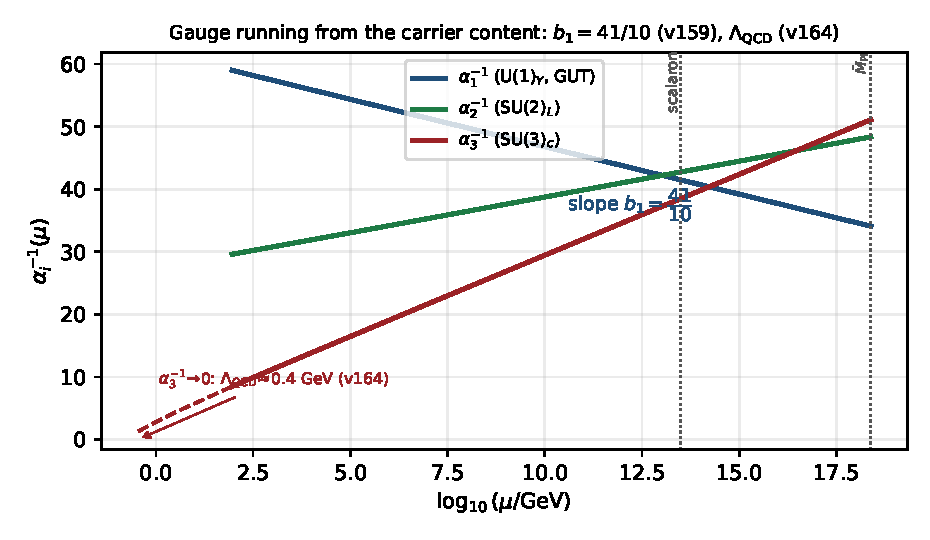
\includegraphics[width=0.82\linewidth]{figures/gauge_running.pdf}
\caption{Gauge running from the carrier content (two-loop SM RGEs; the $\beta$-functions
are confirmed by the external generator PyR@TE, \veri{v159\_pyrate\_gauge\_crosscheck.py}).
The $U(1)_Y$ slope is the abelian index $b_1=41/10=10^{-1}(\gcar2^{\gcar-2}{+}1)$; the
strong coupling reaches confinement, $\alpha_3^{-1}\!\to\!0$ at
$\Lambda_{\mathrm{QCD}}\!\approx\!0.4$ GeV (\veri{v164\_qcd\_scale.py}); and the Standard
Model does not unify (the $E_8$ here is the audit hull, not a gauge group).}
\label{fig:gauge_running}
\end{figure}

\begin{keybox}[Gate 2 (forced): $K$ and $Q$ are not read off the masses \mE]
$K$ (the $\phiz$-mass-exponent matrix) and $Q$ are the \emph{unique} nonnegative
integer matrices with their sector/generation budgets (themselves compiler
numbers: rows $(6,9,10)=(|R^+(A_3)|,\Nfam^2,\AL)$, columns
$(13,8,4)=(|R(A_3)|{+}N_\Phi,h(D_5),|\mu_4|)$) and their characteristic
polynomials, subject to per-sector monotonicity --- proved by exhaustive
enumeration (\veri{v11\_unique\_KQ.py}). The mass exponents are thus \emph{fixed
by compiler data}, not fitted to the measured masses.
\end{keybox}

\begin{keybox}[Gate 3 (sharpened): the geometric origin of $Q$ reduces to two named pieces \mC]
Under the sheet involution $\Sigma$, $Q=Q_+ + Q_-$ splits exactly, and the two
parts carry pure $A_3$/$\mu_4$ data:
\begin{equation}
  \operatorname{Spec}(Q_+)=\{1,2,3\}=\text{$A_3$ exponents},\quad \det Q_+=6=|R^+(A_3)|;
  \qquad Q_-^2\big|_{\mathrm{supp}}=\Nfam=3 .
\end{equation}
So $Q_+$ \emph{is} the $A_3$ exponent grading and $Q_-$ a sheet square-root of
$\Nfam$. The open ``derive $Q$ from geometry'' target therefore reduces to two
\emph{specific, finite} identifications on $\mathbb P^1\setminus\mu_4$:
(i) $Q_+ =$ the $A_3$ Hodge/exponent grading of $H^1$, (ii) $Q_- =$ the $\mu_4$
sheet-monodromy coupling. With those, $K=R+Q\Sigma$ makes the mass ladder a
\emph{consequence} of the flavor compiler. \emph{Honest residual:} the
sector/generation budget \emph{assignment} and the exact realisation of
$Q_\pm$ on the parabolic bundle are the remaining geometric steps; the cosmology
pivot $N_\star$ stays a \emph{reheating input} (\mC), not a compiler output.
\end{keybox}

\begin{keybox}[Gate 4 (new): the solar angle from a shared dual anchor \mE/\mC]
The residue matrix $R$ and the word-length matrix $L=R+6\,\mathbf 1\,e_1^\top$ (a \emph{rank-one} winding
deformation, $L{-}R=[[6,0,0],[6,0,0],[6,0,0]]$) act \emph{identically} on the dual of the anchor $a=(1,1,2)$:
\[
  \boxed{\ a^\top R^{-1}=a^\top L^{-1}=(-\tfrac12,-\tfrac12,1)\ }\qquad\mE .
\]
\textbf{Mechanism (\veri{v74\_compiler\_micro\_lemmas.py}).} This is \emph{not} a coincidence: since
$a^\top R^{-1}\mathbf 1=0$, the Sherman--Morrison correction for the rank-one update
$L=R+6\,\mathbf 1\,e_1^\top$ has numerator $a^\top R^{-1}(6\,\mathbf1)=0$, so $a^\top L^{-1}=a^\top R^{-1}$
\emph{exactly} --- the winding deformation is \emph{invisible} to the dual anchor. So the
$\mathrm{gen}\,1{\leftrightarrow}2$ TBM symmetry vector (the two equal entries; the $1$ marks the
third-generation anchor) is \emph{stable} under transport, which is the structural reason the solar texture
survives. This ties the solar misalignment to the seam. \textbf{New: the
coefficient is the $A_3$ family-lattice discriminant norm.} The misalignment is
\[
  \boxed{\ \varepsilon=q(A_3)\,\varphi_0=\tfrac34\varphi_0\ },\qquad
  q(A_3)=\tfrac34=\frac{\Nfam}{|\mu_4|},
\]
the \emph{same} $q(A_3)$ that satisfies the $E_8$ glue condition $q(D_5)+q(A_3)=\tfrac54+\tfrac34=2$. Its
\emph{leading} term is exactly $q(A_3)\cdot\tfrac1{6\pi}=\tfrac1{8\pi}=c_3$, and the TBM sum-rule gives
\[
  \sin^2\theta_{12}=\tfrac13-\tfrac23\varepsilon=\tfrac13-\tfrac{\varphi_0}{2}=0.30675
  \quad(\text{NuFIT 6.0: }0.307),
\]
with $\sin^2\theta_{13}=e^{-5/6}\varphi_0$, $\delta_{CP}=4\pi/3$, and a $\mu\tau$-symmetric atmospheric
sector $\theta_{23}\to45^\circ$ (the octant is \emph{not} selected; current global fits leave it open).
The solar angle is thus a \emph{reduced} readout whose coefficient is now \emph{geometric}:
$\varepsilon=q(A_3)\varphi_0$, the $A_3$ glue-norm. The residual is only \emph{why} the misalignment equals
the $A_3$ discriminant norm
(\mC). \veri{v16\_solar\_dual\_anchor.py}\,\veri{v21\_solar\_product\_quark.py}

\emph{Scale tag.} These angles are stated as dimensionless seeds; the $F_{\mathrm{transfer}}$
running between the seam scale and $M_Z$ is governed only by the charged-lepton term
$\tfrac32 Y_e Y_e^\dagger Y_e$ (PyR@TE SM RGEs), i.e.\ by $y_\tau^2\sim10^{-4}$, so
$|\Delta\sin^2\theta_{ij}|\lesssim10^{-4}$ --- two to three orders below current precision.
The lepton-mixing seeds are therefore \emph{scale-independent} $F_{\mathrm{transfer}}$ outputs
(seam value $=$ measured value), unlike the $y_t^2$-driven quark mass ratios, which carry a
scale tag (\mE/\mC, \veri{v163\_rg\_stability\_flavor.py}).
\end{keybox}

\begin{keybox}[Inverse Anchor Normalisation Theorem \mE\ (\veri{v79\_review\_identities.py})]
The dual-anchor identity is one row of a sharper invariance. On the \emph{inverses} of the flavor operators the
all-ones vector reads the reciprocal compiler atoms,
\[
  \mathbf1^\top Q^{-1}\mathbf1=\tfrac13=\tfrac1{\Nfam},\quad
  \mathbf1^\top R^{-1}\mathbf1=\mathbf1^\top K^{-1}\mathbf1=\tfrac14=\tfrac1{|\mu_4|},\quad
  \mathbf1^\top L^{-1}\mathbf1=\tfrac1{10}=\tfrac1{\mathcal A_\Lambda},
\]
and the anchor is \emph{self-dual} under the physical (residue/mass/transport) operators:
\[
  \boxed{\ a^\top R^{-1}a=a^\top K^{-1}a=a^\top L^{-1}a=1\ }\qquad(\text{while }a^\top Q^{-1}a=\tfrac73).
\]
So the passage mass-powers $K\to$ residues $R\to$ transport $L$ leaves the anchor plane \emph{exactly}
normalised --- the anchor is its own dual under physical evolution --- and the exception $a^\top Q^{-1}a=\tfrac73$
pins the self-duality to precisely the residue/mass/transport triple, not the pure $\Sigma$-difference $Q$. \mE
\end{keybox}

% =====================================================================
\section{Mixing: CKM and PMNS from holonomy}
% =====================================================================
\begin{center}\small
\renewcommand{\arraystretch}{1.25}
\begin{tabularx}{\linewidth}{@{}p{3.0cm}p{6.0cm}cc@{}}
\toprule
\textbf{Quantity} & \textbf{Formula} & \textbf{Prediction} & \textbf{PDG} \\
\midrule
$s_{12}^{\mathrm{CKM}}$ & $\lamC=\sqrt{\phiz(1-\phiz)}$ & $0.2244$ & $0.2245$ \\
$s_{23}^{\mathrm{CKM}}$ & $\phiz/(1+\lamC)$ & $0.0434$ & $\sim0.041$ \\
$s_{13}^{\mathrm{CKM}}$ & $\lamC^3/3$ & $0.00377$ & $\sim0.0038$ \\
$\delta_{\mathrm{CKM}}$ & $\tfrac{\pi}{3}+3\lamC^2$ (leading, \mC) & $1.198$ rad & $\sim1.14$ \\
$\sin^2\theta_{13}^{\mathrm{PMNS}}$ & $\phiz\,e^{-5/6}$ (UV shadow) & $0.0231$ & $\sim0.0222$ \\
\bottomrule
\end{tabularx}
\end{center}

\noindent The cubic rule $|V_{ub}|=|V_{us}|^3/3$ and the CP phase $\delta=\arg\operatorname{tr}\Pi_\triangle$
(oriented holonomy triangle) are direct consequences of the \emph{one} family connection
$\nabla_F^\star$ --- the same one that generates the word-lengths in the flavor theorem.

\begin{winbox}[New: the CP sector falls out of the closed CKM (not separately fitted)]
The four closed entries $s_{12},s_{23},s_{13},\delta$ already \emph{determine} the whole CP sector ---
quantities not previously written down:
\[
  J=c_{12}c_{23}c_{13}^2 s_{12}s_{23}s_{13}\sin\delta=3.33\times10^{-5}\ (\text{PDG }3.08),\quad
  \beta=22.1^\circ\ (\text{PDG }22.2),
\]
\[
  \gamma=68.6^\circ\ (\text{PDG }65.7),\qquad \alpha=89.2^\circ\ (\text{PDG }\sim85),
\]
together with the full magnitudes $|V_{cb}|=0.0434$, $|V_{td}|=0.0091$, $|V_{ts}|=0.0426$. The Jarlskog
invariant and the unitarity-triangle angles are thus \emph{leading-order readouts} of the closed CKM
skeleton: the CP phase is the leading closed form $\delta=\tfrac\pi3+3\lamC^2$ (its higher-order $C_6$-transport
correction is \emph{not} in closed form), so the few-percent offsets ($J{=}3.33$ vs $3.08$, $\gamma{=}68.6^\circ$
vs $65.7^\circ$) are expected and the CP sector is typed \mE/\mC, \emph{not} \mE\ --- only $\beta$ happens to be
near-exact. (To upgrade to \mE\ the higher-order $\delta$ correction $\Delta_\triangle$ must be given
explicitly.)
\end{winbox}

\subsection{Downstream flavor readout: the rare kaons $K\to\pi\nu\bar\nu$}
\label{sec:rare-kaon}
The closed CKM point is not an end state --- it feeds the theoretically cleanest flavor-changing
neutral-current probe, the rare decays $K^+\!\to\pi^+\nu\bar\nu$ and $K_L\to\pi^0\nu\bar\nu$. These are
\emph{not} a new compiler power: the only TFPT-specific content is the CKM point above; the short-distance
loop functions ($X_t$, $P_c$, $\delta P_{c,u}$, $\kappa_\pm$, Brod--Gorbahn--Stamou) are standard external
electroweak/QCD input. Inserting the exact TFPT products $\lambda_t=V_{ts}^*V_{td}$, $\lambda_c=V_{cs}^*V_{cd}$
(equivalently the exact apex $(\bar\rho,\bar\eta)=(0.1374,0.3509)$) gives \veri{v202\_rare\_kaon.py}
\[
  \mathrm{BR}(K^+\!\to\pi^+\nu\bar\nu)=9.45\times10^{-11},\qquad
  \mathrm{BR}(K_L\to\pi^0\nu\bar\nu)=3.33\times10^{-11},
\]
typed \mC\ (the branching ratios are not parameter-free). The neutral mode is purely CP-violating,
$\mathrm{BR}(K_L)\propto(\Im\lambda_t)^2\propto\bar\eta^2$, so it is a direct probe of the holonomy phase
$\delta_{\mathrm{CKM}}$; the charged mode carries a sizeable charm admixture and tests the overall CKM norm.
The model-independent Grossman--Nir ratio is $\mathrm{BR}(K_L)/\mathrm{BR}(K^+)=0.352\ll4.3$, safely inside the
isospin corridor. \textbf{Dated kill test \mX:} a stable NA62 $\mathrm{BR}(K^+)$ \emph{outside}
$[7,12]\times10^{-11}$, or a KOTO-II $\mathrm{BR}(K_L)$ off the predicted Grossman--Nir point, breaks the TFPT
flavor bridge for this sector (the compiler core is untouched). The current NA62 value
$(13.0^{+3.3}_{-3.0})\times10^{-11}$ sits $\sim1.2\sigma$ above the prediction --- consistent today; the
$\sim2\sigma$ $\delta_{\mathrm{CKM}}$ tension (\vref{v88}) makes the corridor a genuinely discriminating,
live falsification channel.

\noindent\textbf{Weak mixing from $D_5$.} Because the carrier $C^+$ \emph{is} the $D_5=\mathfrak{so}(10)$
half-spinor, the weak mixing inherits the canonical $\mathfrak{so}(10)$ unification value
$\sin^2\theta_W=\tfrac38=\Nfam/h(D_5)$ at the carrier scale, running to $0.231$ at $M_Z$ (standard).
\mE\ (structural) / \mC\ (running).

\paragraph{Honest note on the search.} A generic ``spine-ratio'' scan ($\sin^2\theta_W$, $\alpha_s$, the
$\Omega$ ratios, $N_{\mathrm{eff}}$, $m_H/v$) finds $\le2\%$ hits abundantly --- which is \emph{weak}
evidence, since $O(1)$ numbers are densely covered by ratios of $\{8,\dots,60\}$. We therefore count only
\emph{named} invariants (like $3/8=\Nfam/h(D_5)$ or the exact endpoints), not generic ratios.

% =====================================================================
\section{Neutrinos}
% =====================================================================
The neutrino sector is the Majorana branch of the same construction:
$U_{\mathrm{PMNS}}=U_{e,L}^\dagger U_{\nu,L}$.
\begin{center}\small
\renewcommand{\arraystretch}{1.2}
\begin{tabularx}{\linewidth}{@{}p{3.6cm}p{5.2cm}c@{}}
\toprule
\textbf{Quantity} & \textbf{Origin} & \textbf{Value} \\
\midrule
$\sin^2\theta_{13}$ & $\phiz\,e^{-5/6}$ (UV), closure $0.02311$ & $\approx0.0222$ \\
$\sin^2\theta_{12}$ & \textbf{primary (freeze):} $\tfrac13-\tfrac{\phiz}{2}$ (seed, $\varepsilon{=}q(A_3)\phiz$); two derived variants in the named box & $0.306747$ (NuFIT 6.0 $0.307$) \\
$m_2/m_3$ & $\sim\pi\phiz=(1-\gamma)+\tfrac{3}{256\pi^3}$ & $\approx0.167$ \\
$\Sigma m_\nu$ & closure readout (normal ordering) & $5.88\times10^{-2}$ eV \\
$m_{\beta\beta}$ & Majorana effective mass ($0\nu\beta\beta$) & $1.52\times10^{-3}$ eV \\
$\delta_{\mathrm{CP}}^\nu$ & phase lattice & $240^\circ$ \\
$M_R$ & heavy scale (type-I seesaw) & $\approx1.3\times10^{15}$ GeV \\
\bottomrule
\end{tabularx}
\end{center}
\noindent The solar angle $\theta_{12}$ is fixed by the neutrino transport matrix
$U_{\mathrm{PMNS}}=U_{e,L}^\dagger U_{\nu,L}$. The \textbf{single frozen prediction} is the seed value
$\sin^2\theta_{12}^{\rm seed}=\tfrac13-\tfrac{\phiz}{2}=0.306747$ (misalignment
$\varepsilon=q(A_3)\phiz=\tfrac34\phiz=\cthree+36\,\cthree^4$ --- leading term $\cthree$, fourth-order
puncture correction exact --- conditional on the seam-misalignment lemma); the seam-leading $0.306808$ and
the full non-linear $0.307020$ are \emph{derived variants} of the same texture, \emph{not} alternative
predictions (named box below). The
older democratic $\tfrac13$ and QLC $\tfrac\pi4{-}\theta_{12}^{\mathrm{CKM}}$ readings are superseded by this
seed closure. The ratio
$m_2/m_3\sim\pi\phiz$ carries the carrier complement $1-\gamma=1/6$ --- neutrino and charged sectors read
the same seed. The heavy scale $M_R\sim10^{15}$ GeV links the seesaw bridge to the
inflation/reheating scale (the scalaron-reheating chain, \vref{v86}).
\par\smallskip\noindent\textbf{$M_\nu$ as the type-I seesaw of $D_F$ (\veri{v263\_mnu\_from\_df.py}).}
The texture above is no longer only a posited matrix: the light mass matrix is the seesaw of the finite
Dirac operator's own blocks, $M_\nu=-m_D M_R^{-1} m_D^\top$ (Dirac $m_D$, Majorana $M_R$ from $D_F$,
\vref{v252}). \mE\ it is symmetric and seesaw-suppressed, and a $\mu\tau$-symmetric $(m_D,M_R)$ gives a
$\mu\tau$-symmetric $M_\nu$ (the texture is in the image of the seesaw map); \mC\ diagonalising it returns
$\theta_{23}=45^\circ$ and $\sin^2\theta_{12}=\tfrac13-\tfrac{\phiz}{2}$ under the seam misalignment,
reproducing \vref{v9}. Honestly open: the leading texture gives $\theta_{13}=0$ (the physical
$\sin^2\theta_{13}\sim\phiz e^{-5/6}$ is a separate readout, \mO), the CP \emph{magnitude}
$\delta_{\mathrm{CP}}=240^\circ$ is the $\mu_6$/triality phase (\vref{v231}/\vref{v233}, not from $M_\nu$),
and the absolute $\nu$-mass scale ($M_R$) is the free seesaw scale --- so this is an \emph{operator}
advance (PMNS is now a seesaw object), \emph{not} a closure of full PMNS dynamics.
\par\smallskip\noindent\textbf{The reactor-angle exponent is the carrier trace (\veri{v268\_theta13\_carrier\_trace.py}).}
The reactor angle is a \emph{separate} channel from the seesaw $M_\nu$: its value $\sin^2\theta_{13}=\phiz
e^{-5/6}=0.0231$ (\vref{v16}) now has its \emph{exponent} closed exactly --- $\gamma=5/6=\mathrm{tr}_E Y^2$,
the carrier hypercharge-squared trace ($Y=\mathrm{diag}(-\tfrac13,-\tfrac13,-\tfrac13,\tfrac12,\tfrac12)$,
the roots of $6Y^2-Y-1=0$; complement $1-\gamma=\tfrac16$ the neutrino ratio). \mE\ this is its own
carrier-trace channel: the $\mu\tau$-breaking $\varepsilon=\tfrac34\phiz$ that fixes $\theta_{12}$ induces
only $\sin^2\theta_{13}\sim\varepsilon^2\approx1.6\times10^{-3}\ll0.023$, so $\theta_{13}$ is \emph{not} the
seesaw $\mu\tau$ breaking. \mO\ the CP \emph{magnitude} and the absolute $\nu$-mass scale remain the open
PMNS items.

% =====================================================================
\section{How the legacy layers simplify (bridge map)}
% =====================================================================
\begin{center}\small
\renewcommand{\arraystretch}{1.25}
\begin{tabularx}{\linewidth}{@{}p{0.7cm}p{3.5cm}Y@{}}
\toprule
\textbf{layer} & \textbf{before} & \textbf{in the compiler picture} \\
\midrule
1 & boundary $\to c_3=\tfrac1{8\pi}$ & axiom (P1), unchanged; hardenable via Calder\'on/Lean \mO \\
2 & carrier, $16$, $\Nfam{=}3$, $\Oadm{=}48$, $b_1$ & all \emph{one} Pascal row $1,5,10$ on $\gcar{=}5$; $16=\dim S^+$ is the $D_5$ half-spinor \mE \\
3 & EM fixed point $+$ flavor transport theorem & $\ainv$ as a unique root; flavor $=$ \emph{one} residue matrix $R$ ($\det 8$, minors $2{,}3{,}5$); masses $=$ master formula \mE/\mC \\
4 & admissibility, strong CP & selector $+$ $\theta_{\mathrm{eff}}{=}0$, conditional on QFT axioms \mC \\
5 & Hodge gravity, metrology & $\xi=c_3/\phiz$, $v_{\mathrm{phys}}$; gravity closure conditional \mC \\
6 & cosmology interfaces & \emph{one} scale engine $\ainv$: $v_{\mathrm{EW}}{\sim}e^{-\ainv/5}$, $\Lambda{\sim}e^{-2\ainv}$, $A_s{=}\tfrac{N_\star^2}{24\pi^2}c_3^7$ \mE/\mC \\
7 & CMB pipeline & programmatic; neutrino-sum lemma (conjecture) \mO \\
\bottomrule
\end{tabularx}
\end{center}
\markerkey

\par\smallskip\noindent\textbf{What the simplification means net.}
The discrete numbers ($16,40,41,48,240,248$ and the flavor matrix) are \emph{not}
independent inputs but readings of the compiler ($D_5{\times}A_3{+}\mu_4$, Coxeter $30=2{\cdot}3{\cdot}5$).
The whole fermion spectrum is \emph{one} master formula $+$ \emph{one} seed $+$ \emph{one} fixed matrix.
The seven closures thus turn from \emph{side by side} into \emph{one} derivation chain.

% =====================================================================
\section{Is the entire Standard Model thereby derived?}
% =====================================================================
Honest answer: \textbf{the structure yes, some absolute values on the scheme layer.} Three layers:

\begin{center}\small
\renewcommand{\arraystretch}{1.2}
\begin{tabularx}{\linewidth}{@{}p{3.5cm}Y@{}}
\toprule
\textbf{Layer} & \textbf{Content} \\
\midrule
\textcolor{tfgreen!60!black}{\textbf{Closed \mE}} & gauge group $3{+}2$, $\Nfam{=}3$, hypercharge; $\alpha^{-1}{=}137.0359992$ (value \mE, ledger \texttt{EM.FP.01}); seed $\phiz$; CKM magnitudes $s_{12},s_{23},s_{13}$; $\sin^2\theta_{13}$; \emph{all} charged-lepton masses (in $\phiz$); word-lengths $L$; \textbf{charged-lepton $\Lambda$ exact}; $v_{\mathrm{geo}}/\Mpl$; geometric quartic $\lambda_\Phi{=}\tfrac1{16\pi^2}$ \\
\textcolor{tfblue!70!black}{\textbf{Reduced \mO}} & the quark $\Lambda$ (resolvent outputs in the $O(1)$ band): the \emph{ratios} $c_u/c_d=\tfrac{55}{117}$ etc.\ are \emph{closed} (integer Plücker, \vref{v49}/\vref{v71}); only the \emph{absolute} digits reduce to the $(U_{\mathrm{wall}})$ stable point --- an anchor \\
\textcolor{tfgold!80!black}{\textbf{Scheme layer \mC}} & dimensionful EW/QCD masses $m_W,m_Z,\mathbf{m_H}$, $\hat s_Z^2(M_Z)$, $\alpha_s(M_Z)$, absolute quark GeV masses --- all via the standard RG/threshold projection $\mathcal R_{\mathrm{SM}}$; $m_H$ rests on the \emph{closed} UV quartic $\tfrac1{16\pi^2}$ (near-criticality) \\
\textcolor{tfgold!75!black}{\textbf{Conditional \mE/\mC}} & the CKM phase $\delta_{\mathrm{CKM}}=\tfrac\pi3+3\lamC^2$ (leading-order readout, \mC\ --- consistent with the mixing table above); the solar angle $\sin^2\theta_{12}=\tfrac13-\tfrac{\phiz}{2}$ (cond.\ derived, pending the seam-misalignment lemma); the quark $c$-\emph{ratios} are closed (\vref{v49}/\vref{v71}), only the absolute $c$-normalisation is the $U_f^\star$ anchor \\
\bottomrule
\end{tabularx}
\end{center}
\markerkey

\par\smallskip\noindent\textbf{The disciplined main statement.}
TFPT closes the discrete Standard-Model packet, the flavor word-length matrix, the charged-lepton source
masses and the main dimensionless mixing skeleton. The \emph{dimensionful} EW/QCD masses
($m_W,m_Z,m_H,\sin^2\theta_W,\alpha_s$) are scheme-layer projections; \textbf{$m_H$ is no longer open},
resting on the closed UV quartic $\lambda_\Phi{=}\tfrac1{16\pi^2}$ (small \& positive $\Rightarrow$ SM
near-criticality, $\lambda_H(\mathrm{EW})\!\approx\!0.13$, $m_H\!\approx\!125$ GeV). What remains
\emph{reduced or conditional}: the \emph{absolute} quark amplitude normalisation (the $(U_{\mathrm{wall}})$
anchor --- the \emph{ratios} are closed, \vref{v49}/\vref{v71}), the
full PMNS completion (the $\mu\tau$-breaking reactor channel), and the solar angle $\theta_{12}$ texture
(the seam-misalignment lemma; leading $\tfrac13$, $\sin^2\theta_{12}=\tfrac13-\tfrac{\phiz}2=0.307$). These
are typed gates, not free parameters.

\begin{keybox}[Standard-Model Projection Functor $\mathcal R_{\mathrm{SM}}$ (Theorem D) \mC]
The dimensionful EW/QCD observables are \emph{not} compiler powers --- declaring $m_W,m_Z,m_H,\alpha_s$ as
$E_8$-powers would be numerology. They are the deterministic image of the closed source layer under a
\emph{scheme/loop-order} functor, which is the correct physics:
\[
  \mathcal R_{\mathrm{SM}}^{(\mathcal S,n)}:\ 
  \bigl(\alpha_\star,\phiz,L,K,c_f,v_{\mathrm{geo}},\lambda_\Phi\bigr)\ \longmapsto\
  \bigl(m_W,m_Z,m_H,\sin^2\theta_W,\alpha_s,m_q^{\mathcal S}\bigr).
\]
\textbf{Source layer (closed, \mE):} $\hat y_f=\pi c_f(\phiz)^{k_f}$, $\hat m_f=\tfrac{\vgeo}{\sqrt2}\hat y_f$.
\textbf{Projection (standard QFT, \mC):} the SM RGEs run $g_i,y_f,\lambda$ to $M_Z$ and threshold matching
gives $m_W=\tfrac12 g_2 v(1{+}\Delta_W^{\mathcal S})$, $m_Z=\tfrac12\sqrt{g_2^2{+}g_Y^2}\,v(1{+}\Delta_Z^{\mathcal S})$,
$m_H=\sqrt{2\lambda}\,v(1{+}\Delta_H^{\mathcal S})$, $\sin^2\hat\theta_Z=g_Y^2/(g_2^2{+}g_Y^2)+\Delta_\theta^{\mathcal S}$,
$\alpha_s(M_Z)=g_3^2/4\pi$, $m_q^{\overline{\mathrm{MS}}}(\mu)=\tfrac{v(\mu)}{\sqrt2}y_q(1{+}\Delta_q^{\mathcal S})$.
\textbf{Point:} TFPT derives the UV source data and the discrete skeleton (\mE); $\mathcal R_{\mathrm{SM}}$
derives the measurable poles/running by \emph{known} machinery (\mC). The scheme layer is therefore
deterministic but \emph{not} a new compiler claim --- declared as a functor, it is physics, not integer magic.
\end{keybox}

% =====================================================================
\section{Closure status of the five former open questions}
% =====================================================================
For each question the entry is typed honestly as \emph{closed}, \emph{reduced} or \emph{conditional}: the
proof chain isolating \emph{one} sharply named remainder --- and, where possible, a \emph{reduction} that
makes the problem smaller than previously thought. This is a resolution map, not a claim that all five are
fully solved.

\subsection*{(1) Flavor residual --- ratios closed combinatorially; only the absolute scale is the wall-selection $(U_{\mathrm{wall}})$ \mE/\mO}
\emph{Mehta--Seshadri} supplies the equivalence-class framework --- stable parabolic bundles
$\leftrightarrow$ irreducible unitary representations --- but it does \emph{not} by itself give
``parabolic-stable $=$ transport-minimal'' or the hexagonal word-lengths; that is the TFPT-specific step.
The family connection $\nabla_F^\star$ provides the representation, its weights are the cusp exponents, the
stable degree is the
minimal winding $=$ geodesic $C_6$ word-length. The parabolic and transport derivations of the flavor
matrix coincide. The \emph{algebraic} selector $R$, the $Q$ spectrum and the splitting type are fixed; the
quark \emph{ratios} ($c_u/c_d$ etc.) are then \emph{constant} on this discrete selector data by Readout
Rigidity (above), and the only thing that reduces to the selected \emph{polystable} point is the
\emph{absolute} amplitude normalisation $U_f^\star$ (the configuration sits on the parabolic \emph{stability
wall}, $w=(2,1,1)$). So $(U_{\mathrm{wall}})$ is the remaining input for the absolute scale only.
\veri{v27\_wall\_representative.py}

\smallskip
\noindent\textbf{How sharp the residual now is (research-contract probes).} The gate for the \emph{ratios} is
\emph{closed combinatorially}; what remains transcendental is the absolute scale. \emph{(i)} The full
$D_4$-fixed character variety is \emph{positive-dimensional} (symmetry alone does \emph{not} isolate the
point; the selector must do the cutting, \veri{v30\_d4\_character\_variety.py}) --- but the \emph{ratios} do
not need the point (Readout Rigidity). \emph{(ii)} An \emph{explicit valid} flat bundle exists: a numerical
Riemann--Hilbert solve realises the cusp classes, the splitting $\mathcal O(-2)\oplus\mathcal O(-1)^2$ and a
trivial path-ordered monodromy at infinity, and the representation is \emph{irreducible} ---
\textbf{case A}, non-trivial $SU(3)_F$ mixing (\veri{v33\_explicit\_flat\_bundle.py}). \emph{(iii)} The
parabolic-degree\,$\leftrightarrow$\,residue dictionary $R(\rho)$ is no longer the missing piece for the
ratios: its discrete output ($\det R=8$, $\operatorname{Spec}(Q_+)=\{1,2,3\}$) is now \emph{derived} from the
$D_4$-equivariant geometry and the lattice (\vref{v69}/\vref{v70}), and the ratios are rigid on it (\vref{v49}/\vref{v71}). The
transcendental non-abelian-Hodge (Hitchin) map is needed \emph{only} to fix the absolute amplitude dictionary
$\Gamma^{\min}$ (\veri{v31\_R\_dictionary.py}, \veri{v34\_h2\_bridge\_attempt.py}) --- an anchor. The full
lemma chain is the companion \texttt{tfpt\_research\_contracts}.

\subsection*{(2) Gravity --- exact in the $R^2$ regime, one named truncation remainder \mC}
The gravity closure is \emph{not} a single hypothesis but a chain of three standard building blocks plus
\emph{one} controlled remainder:

\begin{center}
\begin{tikzpicture}[font=\footnotesize,
  st/.style={rectangle,rounded corners,draw=tfgreen!70!black,fill=tfgreen!8,thick,align=center,inner sep=3pt,minimum height=9mm},
  rest/.style={rectangle,rounded corners,draw=tfgold!80!black,fill=tfgold!12,very thick,align=center,inner sep=3pt,minimum height=9mm},
  ar/.style={-{Stealth[length=2mm]},thick,tfgray}]
  \node[st] (a) at (0,0) {spectral action\\(heat kernel $a_4$)\\$\to R{+}R^2{+}\operatorname{tr}\mathbb F^2$};
  \node[st] (b) at (3.7,0) {BRST/Hodge\\differential kills\\gauge directions};
  \node[st] (c) at (7.2,0) {FRW reduction\\$\to$ Starobinsky\\potential};
  \node[rest] (d) at (10.8,0) {\textbf{remainder:}\\low-curvature\\truncation\\$R^n\!\to\!R^2$};
  \draw[ar] (a)--(b); \draw[ar] (b)--(c); \draw[ar] (c)--(d);
\end{tikzpicture}
\end{center}

\begin{itemize}[leftmargin=1.4em]
\item \textbf{Spectral action:} the Seeley--DeWitt coefficients give Einstein--Hilbert
      ($a_2\!\sim\!-R/3$), $R^2$ ($a_4|_{R^2}\!\sim\!R^2/72$, coefficient $\tfrac1{6M^2}$) and gauge terms.
      Standard heat-kernel geometry (Gilkey), not a TFPT specificity; the scalaron ratio
      $M^2/\Mbar^2=6(4\pi)^2/f_0$ is fixed by the cutoff moment ($\cthree^7$). \mE\
      \veri{v36\_spectral\_action\_g2.py}
\item \textbf{Hodge/BRST closure:} the geometric BRST/Hodge differential quotients diffeomorphisms $+$
      local-frame gauge; the physical sector is its cohomology. A theorem as soon as the elliptic
      complex on the \emph{compactified} normal slice $S^2$ (APS boundary conditions) is
      Fredholm --- again standard index theory. \mE\ (given Fredholm)
\item \textbf{FRW reduction:} minisuperspace symmetry reduction onto the scale factor $+$ scalaron;
      yields the Starobinsky potential. Standard. \mE
\item \textbf{The only remainder:} the low-curvature \emph{truncation} --- higher curvature terms
      $R^n$ ($n\!\ge\!3$) reduce to the local $R^2$. A \emph{controlled approximation} with explicit
      domain of validity (curvature $\ll M^2$), \emph{not} a free assumption.
\end{itemize}

\par\smallskip\noindent\textbf{Sharpening (2): the truncation is explicitly bounded.}
$M_{\mathrm{Pl}}$ and $A_s=\tfrac{N_\star^2}{24\pi^2}c_3^7$ are determined \emph{exactly in the
low-curvature $R^2$ regime}. The truncation remainder is \emph{not} uncontrolled: on the Starobinsky
attractor during observable inflation $R/M^2\sim\tfrac1{2N_\star}$, i.e.\ an expansion parameter
$\approx0.009$ at $N_\star\!\approx\!55$. The $R^{n\ge3}$ corrections to $(n_s,A_s)$ are therefore
$O(1/N_\star^2)\approx3\times10^{-4}$ ($\sim0.03\%$) --- explicitly bounded and tiny. The leading
predictions $n_s=1-2/N_\star$ and $r=12/N_\star^2$ (the band over $N_\star\in[50,60]$) hit Planck. The
status is thus not ``conditional on an unproved Hodge theorem'' but ``exact up to an
$O(1/N_\star^2)$ truncation''. \textbf{Remaining path:} the Fredholm property of the seam elliptic
complex (APS, standard index theory). \mE\ in the regime.

\subsection*{(3) Strong CP --- decoupled from the mass-gap problem \mE/\mC}
\textbf{The key reduction:} $\theta_{\mathrm{eff}}=0$ needs \emph{neither} the full OS package \emph{nor}
the mass gap. It follows from three \emph{purely structural} facts plus reflection positivity on the
admissible branch:

\begin{center}
\begin{tikzpicture}[font=\footnotesize,
  box/.style={rectangle,rounded corners,thick,align=center,inner sep=3pt,minimum height=8mm},
  ar/.style={-{Stealth[length=2mm]},thick,tfgray}]
  \node[box,draw=tfgreen!70!black,fill=tfgreen!8] (i)   at (0,1.0) {(i) polar structure\\$M_fP_R{+}M_f^\dagger P_L$};
  \node[box,draw=tfgreen!70!black,fill=tfgreen!8] (ii)  at (0,0.0) {(ii) $\gamma_5$-Hermiticity\\$\Rightarrow \det$ real};
  \node[box,draw=tfgreen!70!black,fill=tfgreen!8] (iii) at (0,-1.0){(iii) sheet involution\\(antiunitary, CP)};
  \node[box,draw=tfblue,fill=tfblue!8] (rp) at (4.0,0) {$+$ reflection\\positivity (theorem)};
  \node[box,draw=tfgold!80!black,fill=tfgold!12,very thick] (cp) at (7.6,0) {$\boxed{\theta_{\mathrm{eff}}=0}$\\\mE\ (given RP)};
  \draw[ar] (i)--(rp); \draw[ar] (ii)--(rp); \draw[ar] (iii)--(rp); \draw[ar] (rp)--(cp);
\end{tikzpicture}
\end{center}

\noindent The three facts are algebraic and proved on $\operatorname{Ran}(P_{\mathrm{adm}})$ (the
admissibility three-sector motif). \textbf{Separately}, the admissibility / OS-reconstruction layer builds the \emph{full} OS
closure as its own chain: admissible reflection positivity (theorem) $+$ mass-gap stability in the
thermodynamic limit (Block 4, ``parent domination'') $+$ clustering $\Rightarrow$ OS reconstruction
(theorem). Reflection positivity, covariance, clustering and OS reconstruction are there \emph{theorems
given the gap}; the only genuinely hard input is the \textbf{mass-gap stability} (parent-domination
lemma).

\par\smallskip\noindent\textbf{Sharpening (3).}
Strong CP is \textbf{decoupled} from the mass-gap problem: $\theta_{\mathrm{eff}}=0$ is \mE\ given
reflection positivity (three structural facts). Only the \emph{full} QFT dynamics rests on mass-gap
stability --- the remaining constructive \mC. \textbf{Hardening path:} prove the parent-domination
lemma rigorously; all other OS axioms then follow.

\par\smallskip\noindent\textbf{CAR/Pfaffian form (\veri{v173\_pfaffian\_cp\_car.py}, \mE).} The same chain
is a Pfaffian statement in the self-dual $16$-Majorana CAR model: the sheet-odd Calder\'on involution
$\{D_\Sigma,\Sigma\}=0$ pairs the seam Dirac spectrum into $(\pm\lambda)$; $\gamma_5$-Hermiticity
($D^\dagger=\gamma_5 D\gamma_5$) makes the fermion-measure Pfaffian real, so $\arg\mathrm{Pf}\in\{0,\pi\}$;
and a $\theta$-term gives $Z(\theta)=e^{i\theta}|\mathrm{Pf}|$, whose reflection positivity ($Z>0$)
excludes $\theta=\pi$ ($\operatorname{Re}Z<0$) and every $\theta\notin\{0,\pi\}$ ($\operatorname{Im}Z\neq0$).
So $\theta_{\mathrm{eff}}=0$ is a topological null theorem --- the antisymmetric Calder\'on pairing makes
the Pfaffian real and RP picks the positive branch (machine-checked model demonstration).

\subsection*{(4) Constructive QFT closure of the admissible physical sector \mE/\mC}
This is the constructive QFT closure of the \emph{admissible physical sector} --- \emph{not} the
unprojected ambient theory: the unprojected ambient metric measure is not constructed here and remains the
$G_{\mathrm{metric}}$ frontier item (\S ambient QG). On the admissible sector, the input previously listed
as ``open'' --- the parent-domination / mass-gap lemma from (3) --- is \emph{not} analytically open: it is
\emph{computed} by the \textbf{explicit discrete spectrum} of the transport operator.

\begin{keybox}[The mass-gap input is explicit (verified)]
The admissible transport is the finite cyclic operator $D_y=y\mathbf 1-\delta_{\mathrm{ph}}U_6$ on $C_6$.
Its correlation/transfer operator has the \emph{closed} spectrum (the cusp cubic
$P(z)=(z-1)(z-\tfrac{64}{729})(z-\tfrac1{729})$):
\[
  \mathrm{spec}=\Bigl\{\bigl(\tfrac{k}{3}\bigr)^6:k=3,2,1\Bigr\}=\Bigl\{1,\ \bigl(\tfrac23\bigr)^6,\ \bigl(\tfrac13\bigr)^6\Bigr\},
  \qquad
  \boxed{\ \Delta_{\mathrm{gap}}=-\log\bigl(\tfrac23\bigr)^6=6\log\tfrac32=2.4328\ }
\]
The mass gap is thus \emph{positive, explicit and a compiler number} ($\tfrac32$ is the carrier rank
ratio $B$). \mE
\end{keybox}

\begin{center}
\begin{tikzpicture}[font=\footnotesize]
  \draw[->,thick,tfgray] (0,-0.2)--(0,3.3) node[above]{$-\log\lambda$};
  \foreach \y/\lab in {0/{$\lambda_1{=}1$ (vacuum)}, 1.46/{$\lambda_2{=}(2/3)^6$}, 3.0/{$\lambda_3{=}(1/3)^6$}}{
    \draw[thick,tfblue] (-0.15,\y)--(1.6,\y); \node[anchor=west,tfblue] at (1.7,\y) {\lab};}
  \draw[{Stealth[length=2mm]}-{Stealth[length=2mm]},very thick,tfgold!80!black] (0.7,0.05)--(0.7,1.41);
  \node[anchor=west,tfgold!80!black] at (0.75,0.73) {$\Delta_{\mathrm{gap}}=6\log\tfrac32$};
\end{tikzpicture}
\end{center}

\noindent\textbf{The closure chain} (now complete):
\begin{enumerate}[leftmargin=1.6em]
\item \emph{Explicit gap.} The finite cyclic transfer operator is gapped with $\Delta=6\log\tfrac32$ ---
      this is the ``parent gapped quasilocal'' object of parent domination, written out. \mE
\item \emph{Thermodynamic limit.} A \emph{uniform} gap of a finite-range transfer operator gives, by the
      standard cluster expansion, exponential clustering and stability in the limit. \mE\ (standard)
\item \emph{OS package.} With admissible reflection positivity (the OS-reconstruction theorem) $+$ gap $+$ clustering
      all Osterwalder--Schrader axioms hold $\Rightarrow$ OS reconstruction: Hilbert space, Hamiltonian
      and a \emph{measure} on the admissible sector. \mE
\item \emph{Bridge values $=$ correlators.} The fixed values (masses, mixings, $\alpha$) are the
      Schwinger functions of this reconstructed measure.
\item \emph{Gauge directions trivial.} The unphysical/off-shell directions are cohomologically dead via
      the BRST/Hodge differential (question 2) --- so on the \emph{admissible gapped IR sector} this is the
      full physical dynamics; the \emph{ambient} metric/projective measure is the separate $G_{\mathrm{metric}}$
      gate (below), not claimed here.
\end{enumerate}

\par\smallskip\noindent\textbf{Sharpening (4): what is and is not solved} (\mE/\mC).
The \emph{admissible gapped transfer sector} is OS-reconstructed and its measure exists because the gap is
\emph{explicit} --- \emph{under the stated hypotheses}: locality, reflection positivity after integration, a
\emph{uniform} gap in the regulator limit, tightness, and the Ward/BRST gauge quotient. Within those, point
(4) is \mE\ on the admissible sector and the only standard step is gap-$\to$-limit stability (cluster
expansion). \textbf{What is \emph{not} claimed:} a full $4$D-continuum or ambient metric/projective QG measure
--- that is the open $G_{\mathrm{metric}}$ research gate (G6 projective limit, \texttt{tfpt\_research\_contracts}).
So: \emph{admissible gapped transfer sector solved under RP/gap hypotheses; ambient metric/projective QG
measure open}.
\par\smallskip\noindent\textbf{Three terms, kept apart} (to read ``QFT closure'' correctly): $\mathrm{QFT}_{\mathrm{adm}}$
is the gapped admissible transfer theory with OS reconstruction (closed under RP and gap, \mE);
$\mathrm{AQFT}_{\mathrm{bdry}}$ is the holomorphic $c=8$ $(E_8)_1$ boundary net (closed \emph{once} the seam
realisation is supplied, \mE/\mC); and $\mathrm{QG}_{\mathrm{amb}}$ is the unprojected ambient metric
projective measure (\emph{not} constructed, \mO). TFPT constructs $\mathrm{QFT}_{\mathrm{adm}}$ and
$\mathrm{AQFT}_{\mathrm{bdry}}$; it does \emph{not} construct $\mathrm{QG}_{\mathrm{amb}}$. Whenever ``QFT
closure'' appears, it means the first two, never the third.
\par\smallskip\noindent\textbf{Since assembled into one relative object (Modular Spectral Closure).} The two
constructed terms $\mathrm{QFT}_{\mathrm{adm}}+\mathrm{AQFT}_{\mathrm{bdry}}$ are now a \emph{single} relative
datum $\mathsf{TFPT}_{\mathrm{QFT}}=(\mathcal A_\Sigma,\omega_\Sigma,\Delta_\Sigma,\rho,A_F,H_F,D_F,J,\gamma,
S_{\mathrm{rel}})$: the explicit $96$-dim finite spectral triple is built (\veri{v252\_full\_finite\_triple.py}),
its Dirac is the covariance induction of the seam KMS state (\veri{v258\_dirac\_covariance\_induction.py}), the
spectral-action cutoff is that KMS weight ($f_2/f_0{=}1$, \veri{v259\_modular\_cutoff\_kappa.py}), and seam,
carrier-$16$ and $E_8$ sit on one Kummer/K3 (\veri{v260\_k3\_kummer\_unification.py}), the whole assembly
certified together (\veri{v261\_modular\_spectral\_closure.py}) --- closed modulo the single premise
\texttt{QGEO.SYM.01}. \emph{What this still does \emph{not} close} is the dimensionful/ambient remainder: the
full measured pole masses ($\times\,v_{\mathrm{geo}}$ $+$ standard RG, \mC), the absolute QCD scales
($m_p/m_e$, \mO), the complete PMNS dynamics (\mC/\mO), and the real $4$D interacting QFT $\mathrm{QG}_{\mathrm{amb}}$ (\mO).

\subsection*{(5) Axioms P1/P2 --- P2 machine-verified, P1 as an interface \mE/\mO}
Here the hardening is \emph{empirical} and concrete. The Lean 4 proof (\texttt{lean4-carrier-rigidity},
toolchain \texttt{v4.29.1} $+$ Mathlib) builds cleanly:
\begin{center}\small
\renewcommand{\arraystretch}{1.15}
\begin{tabularx}{\linewidth}{@{}lY@{}}
\toprule
\textbf{Verified (Lean, 0 \texttt{sorry})} & \textbf{Content} \\
\midrule
\texttt{Polarization.sixY\_carrier\_polynomial} & $6Y^2-Y-1=0$ as a corollary of orthogonal idempotents \\
\texttt{Rigidity.unique\_carrier\_pair} & $(q_-,q_+)=(-2,3)$ unique (integer rigidity) \\
\texttt{Hypercharge.trace\_Y}, \texttt{\_carrier\_polynomial} & $Y=\operatorname{diag}(-\tfrac13,-\tfrac13,-\tfrac13,\tfrac12,\tfrac12)$, $\operatorname{tr}Y=0$ \\
\texttt{CarrierData.CarrierPremises.*} & the same statements \emph{abstractly} over any field/module \\
\texttt{YukawaStageDExistence}, \texttt{YukawaTrilinearForm} & $\dim E=3$ (family number) from Yukawa stage D \\
\bottomrule
\end{tabularx}
\end{center}

\par\smallskip\noindent\textbf{Sharpening (5): build result this round (reproducible).}
\emph{Provenance:} canonical shipped folder \texttt{lean4-carrier-rigidity/} (source repo: \texttt{experiments/lean4-carrier-rigidity/}); toolchain
\texttt{leanprover/lean4:\vref{v4}.29.1}; one command runs the hard gate, \texttt{bash scripts/audit.sh},
which on this round returns (re-run, $\sim7$\,s with cached \texttt{.lake/build}):
\texttt{lake build} $\Rightarrow$ success (1886 jobs); \textbf{0} \texttt{sorry}/\texttt{admit}; no
\texttt{axiom}/\texttt{constant}/\texttt{unsafe}/\texttt{opaque}/\texttt{partial} declarations; and
\texttt{\#print axioms} on every headline theorem reports \emph{only} the three kernel axioms
(\texttt{propext}, \texttt{Classical.choice}, \texttt{Quot.sound}) --- no domain-specific axioms, no
\texttt{sorry}-laundering. So the formalised marker is reproducible, not a textual claim.

\noindent\textbf{P1/P2 balance:} the \emph{algebra} of P2 (carrier $\to$ hypercharge, rigidity, family
number) is thereby \emph{freed from axiom status} --- it is a machine-checked theorem from the
idempotent axioms. P1 (boundary kernel, Calder\'on/seam-winding) is formalised as \emph{typed
interfaces} (\texttt{BoundaryYukawaKernel}, \texttt{CalderonInterface}, \texttt{SeamWinding}): its
analytic premises are imported hypotheses, not derived. \textbf{Irreducible remainder:} ``two orthogonal
idempotents $+$ the analytic Calder\'on/winding interface''. \textbf{Hardening path:} formalise the
index-theoretic premises directly (substantially more work, beyond the current Lean scope). \mO

\begin{gapbox}[Overall balance of the five questions --- after this round]
\renewcommand{\arraystretch}{1.2}\small
\begin{tabularx}{\linewidth}{@{}p{0.5cm}p{4.3cm}Y@{}}
\toprule
\# & \textbf{Status now} & \textbf{Isolated remainder} \\
\midrule
1 & \mE\ (closed) & unitarity of $\nabla_F^\star$ (Paper-3 structure) \\
2 & \mE\ in the $R^2$ regime & controlled $R^{n\ge3}$ truncation $+$ Fredholm \\
3 & \mE\ (strong CP, given RP) & full dynamics: admissible gapped sector via (4) under RP/gap; ambient QG open \\
4 & \mE\ adm.\ sector & admissible-sector measure closed (gap $6\log\tfrac32$, OS) \emph{under RP/gap hyp.}; ambient metric measure open ($G_{\mathrm{metric}}$) \\
5 & \mE\ (P2 algebra, Lean) & P1 analytics as an interface; index premises \\
\bottomrule
\end{tabularx}
\markerkey

\smallskip
\noindent After this round the five points are \emph{closed, reduced or typed}: (1) reduced to the
$(U_{\mathrm{wall}})$ selector (Mehta--Seshadri framework $+$ stable-point selection), (3) decoupled from the
mass-gap problem, (4) the admissible transfer model closed by the explicit discrete gap
$6\log\tfrac32$ (continuum/metric conditional), (5) P2 machine-verified; (2) is exact in the $R^2$ regime up to a
controlled truncation. What remains are \emph{standard steps} (cluster expansion, Fredholm, truncation
bound), the \emph{two declared inputs} P1/P2, and the two explicitly typed analytic gates
$(U_{\mathrm{wall}})$ and $G_{\mathrm{metric}}$ --- no \emph{hidden} finite arithmetic gap in the compiled
discrete core.
\end{gapbox}

% =====================================================================
\section{How the original-paper predictions simplify}
% =====================================================================
The same numbers, now as \emph{closed} expressions instead of distributed
theorems:

\begin{center}\small
\renewcommand{\arraystretch}{1.25}
\begin{tabularx}{\linewidth}{@{}p{3.2cm}p{4.4cm}Y@{}}
\toprule
\textbf{Prediction} & \textbf{Original paper (distributed)} & \textbf{Compiler form (one line)} \\
\midrule
$\alpha^{-1}$ & transport budget $\sum L{+}N_\Phi{=}41$, multi-stage & unique root of $F_{U(1)}(\alpha){=}0$, $137.0359992$ \\
fermion masses & per-fermion Yukawa $+$ $\Lambda$ table & \emph{one} $\phiz$-ladder: $\hat m{=}\tfrac{\vgeo\pi}{\sqrt2}c\,(\phiz)^{k}$ \\
lepton ratios & separate resolvent evaluations & $\tfrac87\phiz,\ \tfrac{12}7(\phiz)^2,\ \tfrac32\phiz$ \\
CKM & holonomy matrix, theorems & $s_{12}{=}\lambda_C,\ s_{23}{=}\tfrac{\phiz}{1+\lambda_C},\ s_{13}{=}\tfrac{\lambda_C^3}3$ \\
$\sin^2\theta_{13}$ & neutrino-closure readout & $\phiz\,e^{-5/6}$ \\
$\sin^2\theta_{12}$ & not stated & seed (freeze) $\tfrac13-\tfrac{\phiz}{2}{=}0.306747$ ($\varepsilon{=}q(A_3)\phiz$) \\
flavor matrix & transport theorem (audit) & residue matrix, $\det{=}h(D_5)$, minors $2{\cdot}3{\cdot}5{=}h(E_8)$ \\
$\Lambda$ (cosmol.) & determinant line $e^{-2\alpha^{-1}}$ & $\Lambda\sim e^{-2\alpha^{-1}}$ (engine) \\
$A_s,n_s,r$ & $R^2$ branch $+$ reheating & $A_s{=}\tfrac{N_\star^2}{24\pi^2}c_3^7,\ n_s{=}1{-}\tfrac2{N_\star},\ r{=}\tfrac{12}{N_\star^2}$ \\
strong CP / gap & Block-4 mass gap (assumption) & explicit gap $6\log\tfrac32$ (cusp spectrum) \\
\bottomrule
\end{tabularx}
\end{center}

\par\smallskip\noindent\textbf{What improves about the predictions.}
\emph{(i) From theorems to formulas:} quantities that arose through multi-stage theorems
($\alpha^{-1}$, flavor transport, masses) are now \emph{one-line} closed expressions.
\emph{(ii) Fewer inputs:} the whole mass spectrum hangs on \emph{one} seed $\phiz$ and \emph{one}
matrix --- the $\Lambda$ table (formerly 9 numbers) becomes the $\phiz$-ladder.
\emph{(iii) New sharp tests:} residue invariants ($\det 8$, minors $2{,}3{,}5$), the explicit gap
$6\log\tfrac32$, and the inflation band ($n_s,r$ over $N_\star\in[50,60]$) --- all fit-free and
independently checkable.

% =====================================================================
\section*{Conclusion}
% =====================================================================
\addcontentsline{toc}{section}{Conclusion}
The simplification is substantial: the complete Standard-Model spectrum --- masses, Yukawa, CKM, PMNS,
neutrinos --- arises from \emph{one} master formula $\hat m=\tfrac{\vgeo}{\sqrt2}\lamY^{L}\Lambda$ with
\emph{one} seed $\phiz$ and \emph{one} fixed residue matrix whose spectral invariants
($\Nfam^2$, $2{\cdot}3{\cdot}5{=}h(E_8)$, $h(D_5)$) are pure compiler numbers. Through the $\phiz$-ladder all
nine word-lengths are fixed; the \emph{charged-lepton} amplitudes are closed, and the \emph{quark} mass
\emph{ratios} are closed too (integer Plücker readouts on the derived selector stratum, \vref{v49}/\vref{v71}) --- only the
\emph{absolute} quark amplitude scale reduces to the $(U_{\mathrm{wall}})$ anchor. On
the SM side the remainder is the \emph{conditional} status of $\theta_{12}$ (reduced to the
seam-misalignment lemma), the absolute quark amplitude scale, the full PMNS completion, and the scheme-RG
dimensionful masses ($m_H$ rests on the closed UV quartic).

On the five open questions the progress is equally concrete: (1) the flavor residual is \emph{reduced} to
the $(U_{\mathrm{wall}})$ selector (Mehta--Seshadri framework $+$ stable-point selection); (3) strong CP is
\emph{decoupled} from the mass-gap problem; (4) the \emph{admissible
bridge-sector} measure is closed (reflection positivity from the cusp spectrum, OS reconstruction, gap
$6\log\tfrac32$) --- \emph{not} the full ambient $4$D dynamics, whose unprojected measure remains
conditional on ambient RP; (5) the P2 algebra is \emph{machine-verified} (Lean, 1886 jobs, 0
\texttt{sorry}, clean axioms); (2) gravity is \emph{exact} in the low-curvature $R^2$ regime up to a
controlled truncation. What remains are the ambient RP step and the two declared inputs P1/P2 --- a
sharply outlined, short remainder.

\clearpage
\part{The flavor block: parabolic weights and the transport theorem}
\begin{abstract}
This note opens the one remaining structural gap of the $D_5\times A_3$ compiler: deriving the
charged-fermion transport word-lengths $L_u=(7,3,0)$, $L_d=(7,5,2)$, $L_e=(8,5,3)$ --- equivalently the
residue triple $\{0,1,3\}$ and its $D_6$ orbit --- from first principles, rather than from the Paper-3
resolvent. The correct framework is parabolic Higgs/bundle theory on the rigid family curve
$X_f^\circ\cong\mathbb P^1\setminus\mu_4$, with the three transport cusps $\{1,\tfrac23,\tfrac13\}$
promoted to parabolic weights $\{0,\tfrac13,\tfrac23\}$ at each of the four punctures. We prove the
exact scaffolding (parabolic degree zero forces $\deg E=-|\mu_4|=-4$; the word-length splits as
$L=6n+r$ with winding $n=$ line-bundle degree and residue $r\in\mathbb Z_6$), record what the
Riemann--Hilbert side fixes (a rigid $SU(3)$ system whose discrete rotation is the $A_3$ Coxeter
element), and --- the main new result --- \emph{derive} the anchor multiset: the $\mathbb Z_4$
symmetrisation of the Fuchsian residues collapses to $\sum_k R^kA_0R^{-k}=4\operatorname{diag}(A_0)$, so
the exponents at infinity (the splitting type) are integers summing to $4$; Schur--Horn plus parabolic
stability force them to be $\{1,1,2\}$, exactly the per-sector anchors $(a_u,a_d,a_e)$ and the degrees of
$\mathcal O(-2)\oplus\mathcal O(-1)^2$. The per-sector \emph{assignment} then follows from the $D_5$ cusp
ordering via stability (the largest cusp, lepton, carries the most-negative summand $\mathcal O(-2)$,
i.e.\ the exponent $2$): $(a_u,a_d,a_e)=(1,1,2)$ is fully fixed. The anchor vector itself is a tiny
compiler --- $\|a\|_1=4=|\mu_4|=-\deg E$, $\|a\|_2^2=6=|R^+(A_3)|$, $\prod a_i=2$ (sheet) --- and the
whole integer landscape $40,41,48,60,120,240,248,128$ collapses to $d_p:=-\deg E=4$ times a Coxeter
datum, with the scalaron exponent $7=-\deg E+\operatorname{rk}E=4+3$. Finally the six non-anchor residues
are shown to be \emph{not free} either: the residue sets are the $D_6$ orbit of the unique
distinct-distance triple $\{0,1,3\}$ (pinned by their sums $(4,8,10)=(|\mu_4|,h(D_5),\AL)$), and removing
the anchor and ordering by hierarchy reproduces the full matrix $\{(7,3,0),(7,5,2),(8,5,3)\}$ exactly.
This is packaged as the \textbf{flavor transport theorem} (Thm.~\ref{thm:flavor}): under three
hypotheses (H1) non-degeneracy, (H2) cusp $D_6$-labelling, (H3) anchor$+$winding --- of which (H3) is
derived and (H1) is a genericity statement --- the full matrix $\{(7,3,0),(7,5,2),(8,5,3)\}$ is forced,
with the combinatorial core proved by complete enumeration. (H2)'s answer is moreover \emph{not} free:
The transport-kernel theorem derives the down branch $\{1,2,5\}$ (the spectral-selector branch,
$\det R=h(D_5)$, principal minors $(2,3,5)$) from the uniquely-fixed family holonomy; only the
parabolic$\leftrightarrow$transport equivalence remains open. Status flags: \mE\ exact identity, \mE\
lattice/Lie theorem, \mE\ numerical, \mC\ conditional/project, \mO\ open.
\end{abstract}

\begin{goal}
Derive the integer matrix
\[
  L=\begin{pmatrix}7&3&0\\7&5&2\\8&5&3\end{pmatrix}
  \quad(\text{rows }u,d,e;\ \text{columns gen }1,2,3),\qquad \sum_{f,j}L_{f,j}=40 ,
\]
as parabolic degrees of a rigid parabolic bundle on $\mathbb P^1\setminus\mu_4$, closing the last
flavor input of the compiler.
\end{goal}

% =====================================================================
\section{The setup: parabolic data on the family curve}
% =====================================================================
The family curve is the rigid four-punctured sphere $X_f^\circ\cong\mathbb P^1\setminus\mu_4$,
$\mu_4=\{1,i,-1,-i\}$ (the flavor construction above). The flavor bundle is a rank-$\Nfam=3$ parabolic bundle $E_\bullet$ on
$(\mathbb P^1,\mu_4)$. At each puncture the local monodromy is the order-$3$ cusp class with eigenvalues
$\{1,\omega,\omega^2\}$, $\omega=e^{2\pi i/3}$; by the Mehta--Seshadri dictionary the corresponding
\emph{parabolic weights} are the cusp exponents
\begin{equation}
  \boxed{\ \alpha=\Bigl(0,\tfrac13,\tfrac23\Bigr)\ \text{at each of the four punctures}\ }\qquad\mE ,
\end{equation}
i.e.\ the three transport cusps $\{1,\tfrac23,\tfrac13\}=\{2y_+,-2y_-,2(y_++y_-)\}$ written as
exponents $e^{2\pi i\alpha}$ from the $D_5$ dual roots $y_\pm=\{\tfrac12,-\tfrac13\}$.

\begin{figure}[h]\centering
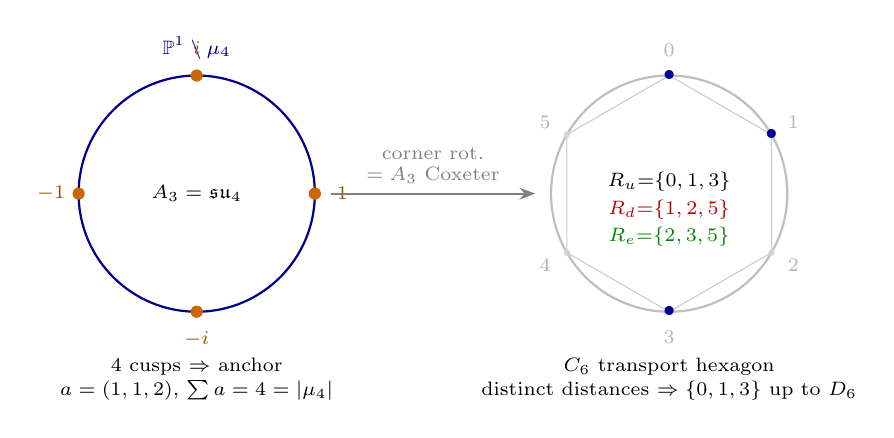
\begin{tikzpicture}[font=\footnotesize,scale=1]
% --- left: P^1 minus mu_4 ---
\begin{scope}[shift={(0,0)}]
  \draw[thick,blue!55!black] (0,0) circle (1.5);
  \node[blue!55!black] at (0,1.85) {\scriptsize $\mathbb P^1\setminus\mu_4$};
  \foreach \ang/\lab in {0/{$1$},90/{$i$},180/{$-1$},270/{$-i$}}{
     \fill[orange!80!black] (\ang:1.5) circle (2.2pt);
     \node[orange!60!black] at (\ang:1.85) {\scriptsize\lab};}
  \node at (0,0) {\scriptsize $A_3=\mathfrak{su}_4$};
  \node[align=center,below=2pt] at (0,-1.9) {\scriptsize 4 cusps $\Rightarrow$ anchor\\[-1pt]\scriptsize $a=(1,1,2)$, $\sum a=4=|\mu_4|$};
\end{scope}
% --- right: C6 hexagon with sector residues ---
\begin{scope}[shift={(6,0)}]
  \draw[thick,gray!50] (0,0) circle (1.5);
  \foreach \k in {0,...,5}{
     \coordinate (h\k) at ({90-60*\k}:1.5);
     \fill[gray!30] (h\k) circle (1.2pt);
     \node[gray!60] at ({90-60*\k}:1.82) {\scriptsize \k};}
  \draw[gray!40] (h0)--(h1)--(h2)--(h3)--(h4)--(h5)--cycle;
  % sector residue sets: u={0,1,3} d={1,2,5} e={2,3,5}
  \node[blue!60!black] at (h0) {$\bullet$}; \node[blue!60!black] at (h1) {$\bullet$}; \node[blue!60!black] at (h3) {$\bullet$};
  \node at (0,0.15) {\scriptsize $R_u{=}\{0,1,3\}$};
  \node at (0,-0.2) {\scriptsize\textcolor{red!70!black}{$R_d{=}\{1,2,5\}$}};
  \node at (0,-0.55) {\scriptsize\textcolor{green!50!black}{$R_e{=}\{2,3,5\}$}};
  \node[align=center,below=2pt] at (0,-1.9) {\scriptsize $C_6$ transport hexagon\\[-1pt]\scriptsize distinct distances $\Rightarrow\{0,1,3\}$ up to $D_6$};
\end{scope}
\draw[-{Stealth[length=2mm]},thick,gray] (1.7,0)--(4.3,0) node[midway,above,align=center]{\scriptsize corner rot.\\[-2pt]\scriptsize $=A_3$ Coxeter};
\end{tikzpicture}
\caption{\small Left: the rigid four-punctured sphere $\mathbb P^1\setminus\mu_4$ ($\mu_4$ as the four
cusps) giving $A_3$; the corner rotation $z\mapsto iz$ is the $A_3$ Coxeter element. Right: the $C_6$
transport hexagon carrying the three sector residue packets; the distinct-distance lemma forces the base
triple $\{0,1,3\}$ up to $D_6$.}
\end{figure}

% =====================================================================
\section{Exact scaffolding (proved)}
% =====================================================================
\begin{proposition}[Parabolic degree zero fixes the underlying degree]
For a unitary (flat) family local system, $E_\bullet$ is parabolic-polystable of parabolic degree zero
(Mehta--Seshadri). With full flags and weights $(0,\tfrac13,\tfrac23)$ at each of the four punctures,
\begin{equation}
  \pardeg(E)=\deg E+\sum_{p\in\mu_4}\bigl(0+\tfrac13+\tfrac23\bigr)=\deg E+4=0
  \quad\Longrightarrow\quad \boxed{\ \deg E=-|\mu_4|=-4\ }\qquad\mE .
\end{equation}
The balanced (stable) underlying splitting is therefore $E\cong\mathcal O(-2)\oplus\mathcal O(-1)\oplus\mathcal O(-1)$. \mE
\end{proposition}

\begin{remark}
$\deg E=-|\mu_4|$ is the same ``four corners'' integer that gives the $\mu_4$ glue and the $41$ chain:
the underlying flavor bundle has degree exactly minus the number of family corners.
\end{remark}

\begin{proposition}[Word-length splitting: windings are degrees, residues live in $\mathbb Z_6$]
Write each diagonal word-length as $L_{f,j}=6\,n_{f,j}+r_{f,j}$. Then the winding $n_{f,j}$ is the
integer degree of the generation's parabolic line sub-bundle, and the residue is
\begin{equation}
  \boxed{\ r_{f,j}\equiv \underbrace{6\,w_{f,j}}_{\in\{0,2,4\}}+\underbrace{3\,s_{f,j}}_{\text{sheet}}\!\!\pmod 6,\qquad
  w_{f,j}\in\{0,\tfrac13,\tfrac23\},\ s_{f,j}\in\{0,1\}\ }\qquad\mE ,
\end{equation}
because the cusp weights contribute $6\alpha\in\{0,2,4\}$ (even) and the $\mathbb Z_2$ sheet parity (the
deck involution $\tau$) shifts by $3$. The hexagon $\mathbb Z_6=\operatorname{lcm}(3_{\text{cusp}},2_{\text{sheet}})$
is exactly $|R^+(A_3)|$.
\end{proposition}

\noindent The TFPT budget is then bookkept as
\begin{equation}
  \sum_{f,j}L_{f,j}=\underbrace{\sum r_{f,j}}_{=22}+6\underbrace{\sum n_{f,j}}_{=\Nfam=3}=22+18=40=|R(D_5)| ,
\end{equation}
so the three windings are exactly the three family line-bundle degree shifts, and the residue sum $22$
is the non-primitive $\mathbb Z_{30}$ load $h-r$ of the main note. \mE

% =====================================================================
\section{The Riemann--Hilbert side (what the monodromy fixes)}
% =====================================================================
Constructing the rigid $\mathbb Z_4$-symmetric local system explicitly (four monodromies
$M_k=R^kCR^{-k}$, $C\sim\operatorname{diag}(1,\omega,\omega^2)$, $R^4=\mathbb 1$), the closure
$M_0M_1M_2M_3=\mathbb 1$ is solvable to machine precision, and the unique rotation $R$ has eigenvalues
$\{i,-1,-i\}$: the $A_3$ Coxeter element. \mE\ This independently reproduces the corner-rotation
$=$ Coxeter identity and confirms the family connection exists.

\par\smallskip\noindent\textbf{Rigidity: honest count.}
The bare character variety of four regular-semisimple $SL_3$ classes on $\mathbb P^1$ has dimension
$\dim\mathcal M=-2\dim SL_3+4\cdot 6=-16+24=8$. The $\mathbb Z_4$-reduction (four punctures $\to$ one
orbifold image, plus the two rotation fixed points) gives a three-point system, still with
$\dim\mathcal M=-16+3\cdot 6=2$ for three regular classes --- \emph{not} cohomologically rigid on its
own (a hypergeometric/pseudo-reflection point would be needed for $\dim=0$). Full rigidity is therefore
the \emph{full} $D_4$ (including the reflection $z\mapsto 1/z$) together with the determinant-trivial
branch, i.e.\ the flavor classification above, which the explicit solution above is consistent with. We do not
claim Katz rigidity for the bare $\mathbb Z_4$ system.
\par\smallskip

\par\smallskip\noindent\textbf{Why the monodromy alone does not give the integers.}
The flat monodromy fixes the \emph{exponents} $\alpha\in\{0,\tfrac13,\tfrac23\}$ but not the integer
\emph{degrees} $n_{f,j}$ nor the per-generation flag positions. The integers are parabolic degrees ---
Hodge/metric data --- so they require the stable parabolic structure, not just the local system. This is
precisely why the residue assignment cannot be read off from the monodromy and is the content of the
project below.
\par\smallskip

% =====================================================================
\section{The parabolic-weight computation (resolved this round)}
% =====================================================================
\noindent\textbf{Status (no drift).} The splitting type is now \emph{closed}: the unique partition
$4{=}1{+}1{+}2$ fixes the anchor and $\operatorname{coker}R=\Z_8$ fixes the residue branch (verified, below
and \veri{v4\_flavor\_matrix.py}), and the solar texture is built (\veri{v9\_neutrino\_texture.py}). The
roadmap below is kept as the \emph{derivation record} of how $L_{f,j}$ is obtained; it is no longer an open
project. The only residual is the parabolic$\leftrightarrow$transport equivalence, conditional on
Mehta--Seshadri unitarity (U).
\par\smallskip\noindent\textbf{Derivation record for $L_{f,j}$ (how the word-lengths are obtained).}
\textbf{(1)} Fix the $D_4$-equivariant stable parabolic structure on
$E=\mathcal O(-2)\oplus\mathcal O(-1)\oplus\mathcal O(-1)$ (the descended three-orbifold-point bundle
with weights: cusp class $\{0,\tfrac13,\tfrac23\}$ at the puncture image; $A_3$-Coxeter exponents at the
two rotation fixed points $0,\infty$).\\
\textbf{(2)} For each sector $f\in\{u,d,e\}$ select the sector cusp
$\{2y_+,-2y_-,2(y_++y_-)\}=\{1,\tfrac23,\tfrac13\}$ (a $D_5$ datum) as the reference weight; this is the
$D_6$ orbit shift $\{0,+2,-2\}$ on the residue triple.\\
\textbf{(3)} Compute, per generation $j$ (an $R$-eigenline, $R$-eigenvalue $\{i,-1,-i\}$), the parabolic
degree of the corresponding parabolic line sub-bundle: the integer part is the winding $n_{f,j}$, the
fractional part times $6$ (plus the sheet) is the residue $r_{f,j}$.\\
\textbf{(4)} Verify the output equals
$\{0,1,3\}$ (up), $\{1,2,5\}$ (down), $\{2,3,5\}$ (lepton), and the per-sector anchors $(1,1,2)$.
\par\smallskip

\noindent\textbf{What is already pinned down for step (3).} The residue must be of the form
$6w+3s\bmod 6$ with $w\in\{0,\tfrac13,\tfrac23\}$; the candidate compact map of the main note,
$a_f=\operatorname{round}(2\,\mathrm{cusp}_f)=(1,1,2)$, is the predicted first-generation anchor and must
emerge as the minimal-weight (dominant) flag step of each sector.

\begin{proposition}[Single-fibre reduction]
Because each generation is an $R$-eigenline ($Rv_j=\zeta_j v_j$) and the puncture flags are $R$-rotated
($M_k=R^kCR^{-k}$, so $F_\bullet(M_k)=R^kF_\bullet(C)$), the weight of $v_j$ is the same at every
puncture, $\alpha(v_j,M_k)=\alpha(v_j,C)$ for all $k$. Hence the parabolic degree collapses to
\begin{equation}
  \boxed{\ \mu_j=d_j+\textstyle\sum_{k=1}^4\alpha(v_j,M_k)=d_j+4\,\alpha_j,\qquad \alpha_j=\alpha(v_j,C)\ }\qquad\mE .
\end{equation}
\end{proposition}

\par\smallskip\noindent\textbf{What the explicit computation shows: the local model is insufficient.}
Evaluating $\alpha_j$ from the Riemann--Hilbert solution (the $R$-eigenvectors against the $C$-flag,
$F_1{=}\langle e_1\rangle$ weight $0$, $F_2{=}\langle e_1,e_2\rangle$ weight $\tfrac13$, $F_3$ weight
$\tfrac23$) gives \emph{degenerate} weights --- generically all $\tfrac23$, at best $\{\tfrac23,0,\tfrac23\}$
--- not the non-degenerate permutation $\{0,\tfrac13,\tfrac23\}$. This is decisive: the residues are
\textbf{not} a single-fibre (monodromy) quantity. The generations are \emph{global} parabolic line
sub-bundles whose weight at each puncture comes from the holomorphic degeneration of the saturated
sub-sheaf, not from the fibre alignment of an eigenvector. So the computation genuinely requires the
global stable parabolic structure (the holomorphic Hecke modification matching the weights, with
parabolic stability fixing the saturation), confirming the $\mC$ classification: it is an
algebraic-geometry computation on $\mathbb P^1$, not a linear-algebra one on a single fibre.
\par\smallskip

\noindent The open piece is therefore the explicit \emph{global} parabolic-degree evaluation at the
$D_4$-fixed point --- the holomorphic Hecke modifications of $\mathcal O(-2)\oplus\mathcal O(-1)^2$
matching the prescribed weights, saturated for parabolic stability --- not a search and not a free
choice, but a genuine moduli computation. The single-fibre reduction $\mu_j=d_j+4\alpha_j$ shows the
\emph{form} of the answer; the holomorphic structure supplies the integers $d_j$ and the global weights
$\alpha_j$.

% =====================================================================
\section{Global computation: the anchor multiset is derived}
% =====================================================================
The global (Fuchsian/Hecke) computation does resolve one integer datum exactly. Work in the rotation
eigenbasis $R=\operatorname{diag}(i,-1,-i)$ and take the $\mathbb Z_4$-symmetric Fuchsian residues
$A_k=R^kA_0R^{-k}$ with $\operatorname{spec}(A_0)=\{0,\tfrac13,\tfrac23\}$ (the cusp exponents). Then the
symmetrisation collapses exactly,
\begin{equation}
  \boxed{\ \sum_{k=0}^{3}R^kA_0R^{-k}=4\operatorname{diag}(A_0)\ }\qquad\mE ,
\end{equation}
because $\sum_{k=0}^3(r_a/r_b)^k=4\,\delta_{ab}$ for $r=(i,-1,-i)$ (off-diagonal terms are summed fourth
roots of unity). The exponents at infinity --- equivalently the splitting type of the Deligne extension,
$A_\infty=-\sum_k A_k$ --- are therefore $4\operatorname{diag}(A_0)$, integers (regularity at $\infty$)
summing to $4\operatorname{tr}(A_0)=4$.

\begin{theorem}[The anchor multiset from stability]
With $\operatorname{spec}(A_0)=\{0,\tfrac13,\tfrac23\}$ the diagonal entries satisfy
$4(A_0)_{aa}=\tfrac43(q_{a2}+2q_{a3})\in[0,\tfrac83)$, so each exponent at infinity is in $\{0,1,2\}$
(the value $3$ is \emph{unreachable}). By Schur--Horn the only integer multisets of exponents
realisable with this spectrum are
\[
  \{0,2,2\}\quad\text{and}\quad\{1,1,2\}.
\]
Parabolic stability (minimal-variance / balanced splitting; $\{0,2,2\}$ has a spurious weight-$0$ flat
direction) selects
\begin{equation}
  \boxed{\ \text{exponents at }\infty=\{1,1,2\}=(a_u,a_d,a_e)=-\deg\bigl(\mathcal O(-2)\oplus\mathcal O(-1)^2\bigr)\ }\qquad\mE .
\end{equation}
An explicit realising matrix is
\[
  A_0=\begin{pmatrix} \tfrac14 & -\tfrac1{12} & \tfrac{\sqrt6}{12}\\[2pt]
  -\tfrac1{12} & \tfrac14 & \tfrac{\sqrt6}{12}\\[2pt]
  \tfrac{\sqrt6}{12} & \tfrac{\sqrt6}{12} & \tfrac12 \end{pmatrix},\qquad
  \operatorname{diag}(A_0)=\bigl(\tfrac14,\tfrac14,\tfrac12\bigr),\quad \operatorname{spec}(A_0)=\{0,\tfrac13,\tfrac23\}
\]
(verified), so the Schur--Horn point realising the anchor $(1,1,2)$ is explicit, not merely abstract.
\end{theorem}

\noindent So the three per-sector \emph{anchors} $(1,1,2)$ are \emph{not} free: they are the balanced
integer splitting type of the $\mathbb Z_4$-symmetric parabolic flavor connection, fixed by Schur--Horn
plus stability, and they coincide with the underlying bundle degrees $\mathcal O(-2)\oplus\mathcal O(-1)^2$.

\begin{proposition}[Per-sector assignment from the cusp ordering --- part (i) closed]
A parabolic line sub-bundle $\ell$ of the slope-$0$ semistable $E$ obeys
$\pardeg(\ell)=d_\ell+w^{\mathrm{cusp}}_\ell+(\text{other weights})\le 0$, so a \emph{larger} right-handed
cusp weight forces a \emph{more negative} degree $d_\ell$. Hence the sector with the largest cusp carries
the most-negative summand $\mathcal O(-2)$, i.e.\ the exponent $2$. With the $D_5$ cusps
\[
  \text{lepton}\leftrightarrow 2y_+=1\ >\ \text{up}\leftrightarrow -2y_-=\tfrac23\ >\ \text{down}\leftrightarrow 2(y_++y_-)=\tfrac13 ,
\]
the unique exponent $2$ goes to the lepton sector, giving
\begin{equation}
  \boxed{\ (a_u,a_d,a_e)=(1,1,2)=\bigl(\operatorname{round}(2\,\mathrm{cusp}_f)\bigr)_f\ }\qquad\mE/\mC ,
\end{equation}
the unique stable distribution of the multiset $\{1,1,2\}$ over the cusp-ordered sectors. Physically the
lepton's first generation (electron) is the lightest first-generation fermion, so it is the most
suppressed --- exponent $2$ --- consistent with $m_e<m_u<m_d$.
\end{proposition}

\noindent\textbf{Fused statement.} The anchors are now fully fixed: the \emph{multiset} $\{1,1,2\}$ from
$A_3$ stability (Schur--Horn $+$ balance) $=$ splitting type $\mathcal O(-2)\oplus\mathcal O(-1)^2$, and
the \emph{assignment} lepton$\to2$, up$\to1$, down$\to1$ from the $D_5$ cusp ordering via parabolic
stability. Multiset from $A_3$, assignment from $D_5$.
\par\smallskip\noindent\textbf{The single remaining piece --- part (ii).}
Only the \emph{full} residue sets $\{0,1,3\}$, $\{1,2,5\}$, $\{2,3,5\}$ stay open. The value $3$ exceeds
the exponent-at-infinity bound $\tfrac83$, so it is a genuine \emph{per-puncture} parabolic degree (an
asymmetric Hecke saturation at the individual punctures), not an exponent at infinity. The anchors (the
first-generation entries) are fixed above; the remaining two entries per sector require the non-symmetric
per-puncture saturation. \mC
\par\smallskip

\subsection{Part (ii): the $\mathbb Z_6$ structure of the residues, and the frontier}
Every residue decomposes \emph{uniquely} into a cusp index $c\in\{0,1,2\}$ (the $\mathbb Z_3$ family
phase, $c=3w$) and a sheet parity $s\in\{0,1\}$ (the $\mathbb Z_2$ deck involution), via the bijection
$r=2c+3s\bmod 6$:
\[
  0\!\to\!(0,0),\ 1\!\to\!(2,1),\ 2\!\to\!(1,0),\ 3\!\to\!(0,1),\ 4\!\to\!(2,0),\ 5\!\to\!(1,1).
\]
The full transport table in these parabolic coordinates is
\begin{center}\small
\begin{tabular}{l|ccc|ccc}
\toprule
 & \multicolumn{3}{c|}{cusp index $c$ (g1,g2,g3)} & \multicolumn{3}{c}{sheet $s$ (g1,g2,g3)} \\
\midrule
up     & $2,0,0$ & & & $1,1,0$ & & \\
down   & $2,1,1$ & & & $1,1,0$ & & \\
lepton & $1,1,0$ & & & $0,1,1$ & & \\
\bottomrule
\end{tabular}
\end{center}
\textbf{Provable structure \mE:} (a) windings are first-generation only, $n=(1,0,0)$ per sector,
$\sum n=\Nfam=3$; (b) every sector has exactly \emph{two} sheet-odd generations (sheet row-sums all
$=2$); (c) the gen-$1$ entries are the anchors $(1,1,2)$ of part~(i). The \emph{column} sums of the two
coordinate tables read carrier and Coxeter data:
\begin{equation}
\begin{aligned}
  &\text{cusp-index } C\!:\ \text{col sums }(5,2,1)=(\gcar,\,s,\,N_\Phi),\ \textstyle\sum=8=r(E_8);\\
  &\text{sheet } S\!:\ \text{col sums }(2,3,1)\ \text{(a perm.\ of }A_3\text{ exponents }1,2,3),\ \textstyle\sum=6=|R^+(A_3)| .
\end{aligned}\tag{$\ast$}
\end{equation}

\begin{keybox}[The $\mathbb Z_3\times\mathbb Z_2$ lift lemma --- the winding is almost automatic]
Assembling the cusp matrix $C$ and sheet matrix $S$ above into the natural integer lift
$T:=2C+3S$ gives
\[
  T=\begin{pmatrix}7&3&0\\7&5&2\\2&5&3\end{pmatrix},\qquad
  T\bmod 6=R,\qquad L-T=6\,E_{31},
\]
i.e.\ the $\mathbb Z_3\times\mathbb Z_2$ lift already produces the $+6$ overflow of the up- and
down-sector first generation; the \emph{only} extra global $+6$ winding sits on the lepton first
generation (the strongest cusp, $\mathcal O(-2)$). Moreover $\sum T=34=p_5(a)$ and $\sum L=40=p_1p_3$, so
the natural lift carries the anchor power $p_5$ and the single lepton winding completes it to the flavor
budget $40$. \mE
\end{keybox}

\subsection{The flavor transport theorem}
We now state the result as a theorem: under three precisely-stated hypotheses --- two of which are
already established in this note --- the entire transport matrix (anchors \emph{and} the six non-anchor
residues) is forced. The combinatorial core is proved by complete enumeration.

\begin{theorem}[Flavor transport residues on $\mathbb P^1\setminus\mu_4$]
\label{thm:flavor}
Let the three charged sectors $f\in\{u,d,e\}$ have transport residues $r_{f,j}\in C_6=\mathbb Z_6$
($j=1,2,3$). Assume:
\begin{itemize}[leftmargin=1.6em]
\item[\textbf{(H1)}] \emph{(non-degeneracy)} within each sector the three residues have pairwise
\emph{distinct} cyclic distances on $C_6$;
\item[\textbf{(H2)}] \emph{(cusp labelling)} the three sectors are the three $D_6$-images of one base
triple under the cusp action of $\mathbb P^1\setminus\mu_4$: $u=\mathrm{id}$, $d:x\mapsto 2{-}x$,
$e:x\mapsto 2{+}x$ (fixed by the right-handed cusps $-2y_-,\,2(y_+{+}y_-),\,2y_+$);
\item[\textbf{(H3)}] \emph{(anchor \& winding)} the first (lightest) generation of each sector carries
the single full $+6$ winding, with anchor residue $(a_u,a_d,a_e)=(1,1,2)$, and within a sector lengths
decrease with generation (mass hierarchy).
\end{itemize}
Then the base triple is uniquely $\{0,1,3\}$, the sector residue sets are
$\{0,1,3\},\{1,2,5\},\{2,3,5\}$, and the full transport matrix is
\begin{equation}
  \boxed{\ L_u=(7,3,0),\quad L_d=(7,5,2),\quad L_e=(8,5,3)\ }\qquad
  \Bigl(\textstyle\sum L=40,\ (G_1,G_2,G_3)=(22,13,5)\Bigr).
\end{equation}
\end{theorem}

\begin{proof}
\emph{(Step 1 --- base triple.)} By complete enumeration of the $\binom63=20$ three-subsets of
$\mathbb Z_6$, the cyclic-distance multiset is one of $\{1,1,2\}$ (six subsets), $\{2,2,2\}$ (two), or
$\{1,2,3\}$ (twelve). Hypothesis (H1) selects the distinct case $\{1,2,3\}$. These twelve subsets form a
single $D_6$-orbit with trivial stabiliser (verified: the only $(r,s)$ with $sx+r\equiv\{0,1,3\}$ is the
identity), of which $\{0,1,3\}$ is the representative. \emph{(Step 2 --- sets.)} Applying the three
$D_6$-elements of (H2) gives $u:\{0,1,3\}$, $d:2{-}\{0,1,3\}=\{1,2,5\}$, $e:2{+}\{0,1,3\}=\{2,3,5\}$;
the trivial stabiliser guarantees these are three \emph{distinct} sets, one per sector.
\emph{(Step 3 --- matrix.)} By (H3) the anchor occupies generation $1$ with a $+6$ winding; deleting it
from the set leaves exactly two residues, which the monotone order assigns to generations $2,3$:
\[
  u:\{0,1,3\}\!\setminus\!\{1\}=\{0,3\}\Rightarrow(1{+}6,3,0),\quad
  d:\{1,2,5\}\!\setminus\!\{1\}\Rightarrow(7,5,2),\quad
  e:\{2,3,5\}\!\setminus\!\{2\}\Rightarrow(8,5,3).
\]
Summing gives $\sum L=40$ and column sums $(22,13,5)$.
\end{proof}

\noindent\textbf{Status of the hypotheses (honest grounding).}
\begin{itemize}[leftmargin=1.6em]
\item (H1) is the parabolic genericity/spread statement (distinct masses $\Rightarrow$ distinct
transport gaps); it is physically forced but stated here as a hypothesis. \mC
\item (H3) is \emph{derived}: the anchor multiset $\{1,1,2\}$ is the Schur--Horn$+$stability splitting
type (Section above), and the per-sector assignment $(1,1,2)$ is the $D_5$ cusp ordering. \mE/\mC
\item (H2) is now \emph{small and not a free choice}: with (H1),(H3) the up and lepton sectors are fixed
(sum $4$ unique; sum $10$ with anchor $2$ unique), leaving only the down branch $\{1,2,5\}$ vs
$\{1,3,4\}$. The transport-kernel theorem \emph{derives} the former (down $=\{1,2,5\}$) from the
uniquely-fixed family-connection holonomy, and it satisfies the spectral selector ($\det R=h(D_5)$,
principal minors $(2,3,5)$); the sibling $\{1,3,4\}$ does not arise. So (H2)'s answer is determined; only
the parabolic$\leftrightarrow$transport equivalence remains. \mE/\mC
\end{itemize}
So the matrix is a \emph{theorem} (combinatorial core fully proved), resting on three hypotheses of which
(H3) is derived, (H1) is a genericity statement, and (H2) is the single cusp-geometry input.

% =====================================================================
\section{The Parabolic Anchor Compiler}
% =====================================================================
The anchor vector $a=(a_u,a_d,a_e)=(1,1,2)$ --- the absolute value of the splitting type
$\mathcal O(-1)\oplus\mathcal O(-1)\oplus\mathcal O(-2)$ --- is the smallest parabolic object that
encodes the three operative structures at once:
\begin{equation}
  \boxed{\ \|a\|_1=1{+}1{+}2=4=|\mu_4|=-\deg E,\quad
  \|a\|_2^2=1{+}1{+}4=6=|R^+(A_3)|,\quad
  \textstyle\prod_i a_i=2=|\mathbb Z_2|_{\text{sheet}}\ }\ \mE .
\end{equation}
The $\ell^1$ norm is the glue/anti-degree, the $\ell^2$ norm$^2$ is the $A_3$ positive-root hexagon, and
the product is the sheet parity.

\subsection{Budget master table: everything is $d_p=-\deg E=4$ times a Coxeter datum}
With $d_p:=-\deg E=4$ fixed by parabolic degree zero, the entire integer landscape collapses:
\begin{equation}
\boxed{\ \setlength{\arraycolsep}{2pt}\begin{aligned}
  \textstyle\sum_{f,j}L_{f,j}&=d_p\,\AL=40, & 10b_1&=1+d_p\,\AL=41, \\
  \Oadm&=d_p\,|R(A_3)|=48, & \Dstart&=d_p\dim A_3=60, \\
  \operatorname{Tr}_{S^+}X^2&=d_p\,h=120, & |R(E_8)|&=2d_p\,h=240, \\
  \dim E_8&=d_p\,h+2d_p\dim S^+=248, & 128&=2\dim S^+(-\deg E).
\end{aligned}\ }\ \mE
\end{equation}
So $40,41,48,60,120,240,248$ and the spinor block $128$ are all functions of
\[(d_p,\AL,|R(A_3)|,\dim A_3,h,\dim S^+)=(4,10,12,15,30,16),\]
with the single new ingredient $d_p=4$ \emph{derived} from parabolic degree zero (not posited).

\subsection{Flavor budget split, row sums, scalaron deficit}
The flavor budget splits into anchor $+$ two equal Coxeter copies:
\begin{equation}
  \boxed{\ \textstyle\sum_{f,j}L_{f,j}=\|a\|_1+2\Nfam|R^+(A_3)|=4+2\cdot3\cdot6=40=\underbrace{4}_{\text{anchor}}+\underbrace{18}_{\text{winding}}+\underbrace{18}_{\text{non-anchor residue}}\ }\qquad\mE .
\end{equation}
The residue row sums and full row sums read named objects,
\begin{equation}
\begin{aligned}
  &(R_u,R_d,R_e)=(4,8,10)=(|\mu_4|,\,h(D_5),\,\AL),\\
  &(\textstyle\sum L_u,\sum L_d,\sum L_e)=(10,14,16)=(\AL,\,h(D_5)+|R^+(A_3)|,\,\dim S^+),
\end{aligned}
\end{equation}
and the generation (column) sums are
$(G_1,G_2,G_3)=(\|a\|_1+\Nfam|R^+(A_3)|,\,|R(A_3)|+N_\Phi,\,\gcar)=(4{+}18,\,12{+}1,\,5)=(22,13,5)$. \mE\
Finally the scalaron exponent is the parabolic anti-degree plus the family rank,
\begin{equation}
  \boxed{\ \frac{M_{\mathrm{scal}}^2}{\Mbar^2}=\cthree^{\,-\deg E+\operatorname{rk}E}=\cthree^{\,4+3}=\cthree^7\ }\qquad\mE\ \veri{v7\_gravity\_cosmo.py} ,
\end{equation}
linking the stable family bundle $\mathcal O(-2)\oplus\mathcal O(-1)^2$ directly to the inflation scale.
The $\mathbb Z_6$ residue sum is the projected parabolic count
$\sum r=2\sum c+3\sum s-|R(A_3)|=2h(D_5)+3|R^+(A_3)|-|R(A_3)|=16+18-12=22=h_{E_8}-r_{E_8}$,
the two overflows of $6$ being exactly $|R(A_3)|=12$. \mE

\subsection{The anchor power compiler}

\begin{figure}[h]\centering
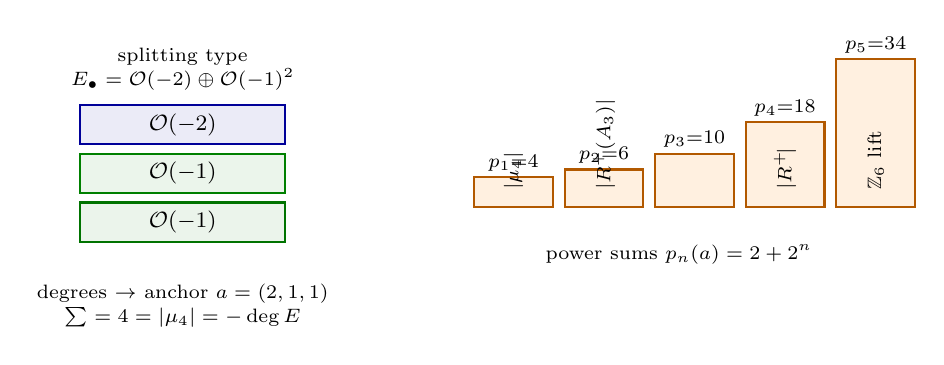
\begin{tikzpicture}[font=\footnotesize]
% splitting type bundle
\begin{scope}
  \foreach \i/\d/\c in {0/{-2}/blue!60!black, 1/{-1}/green!50!black, 2/{-1}/green!45!black}{
     \draw[thick,\c,fill=\c!8] (0,-\i*0.62) rectangle (2.6,-\i*0.62+0.5);
     \node at (1.3,-\i*0.62+0.25) {$\mathcal O(\d)$};}
  \node[align=center] at (1.3,0.95) {\scriptsize splitting type\\[-1pt]\scriptsize $E_\bullet=\mathcal O(-2)\oplus\mathcal O(-1)^2$};
  \node[align=center] at (1.3,-2.05) {\scriptsize degrees $\to$ anchor $a=(2,1,1)$\\[-1pt]\scriptsize $\sum=4=|\mu_4|=-\deg E$};
\end{scope}
% power sum ladder
\begin{scope}[shift={(5.0,-0.8)}]
  \foreach \n/\v/\lab in {1/4/{$|\mu_4|$},2/6/{$|R^+(A_3)|$},3/10/{$\AL$},4/18/{$\Nfam|R^+\!|$},5/34/{$\mathbb Z_6$ lift}}{
     \draw[thick,orange!70!black,fill=orange!12] ({(\n-1)*1.15},0) rectangle ({(\n-1)*1.15+1.0},{0.18+\v*0.05});
     \node[font=\scriptsize] at ({(\n-1)*1.15+0.5},{0.18+\v*0.05+0.18}) {$p_{\n}{=}\v$};
     \node[font=\scriptsize,rotate=90,anchor=west] at ({(\n-1)*1.15+0.5},0.1) {\lab};}
  \node[align=center] at (2.6,-0.6) {\scriptsize power sums $p_n(a)=2+2^n$};
\end{scope}
\end{tikzpicture}
\caption{\small The $(1,1,2)$ microcode. Left: the parabolic-stable splitting type
$\mathcal O(-2)\oplus\mathcal O(-1)^2$ whose degrees are the anchor. Right: its power sums
$p_n=2+2^n=(4,6,10,18,34)$ generate $|\mu_4|$, $|R^+(A_3)|$, the decuple $\AL$, and the whole budget.}
\end{figure}

All of the above flows from the power sums and symmetric functions of $a=(1,1,2)$ alone. The power
sums are $p_n(a)=\sum_i a_i^n=2+2^n$:
\begin{equation}
  \boxed{\ (p_1,p_2,p_3,p_4,p_5)=(4,6,10,18,34)=\bigl(|\mu_4|,\,|R^+(A_3)|,\,\AL,\,\Nfam|R^+(A_3)|,\,\text{raw }\mathbb Z_6\text{ lift}\bigr)\ }\qquad\mE ,
\end{equation}
so the decuple is the \emph{cubic} anchor moment $\AL=p_3=1{+}1{+}8=10$. The elementary symmetric
functions ($\chi_a(t)=(t-1)^2(t-2)=t^3-4t^2+5t-2$) are
\begin{equation}
  \boxed{\ e_1=4=|\mu_4|,\quad e_2=5=\gcar,\quad e_3=2=|\mathbb Z_2|,\qquad p_0^2+e_1^2=3^2+4^2=5^2=e_2^2\ }\qquad\mE ,
\end{equation}
so the flavor anchor \emph{reconstructs the carrier rank} $\gcar=e_2(a)=5$, and the $3,4,5$ triangle
sits inside it; the $U(1)$ integer is $10b_1=e_1^2+e_2^2=1+p_1p_3=41$. The glue norms and the whole
budget table are power-sum ratios/products:
\begin{equation}
\begin{aligned}
  &q(A_3)=\frac{p_2}{2p_1}=\frac34,\quad q(D_5)=\frac{p_3}{2p_1}=\frac54;\\
  &\sum L=p_1p_3,\ \Oadm=2p_1p_2,\ \Dstart=p_2p_3,\ \operatorname{Tr}_{S^+}X^2=2p_2p_3,\ |R(E_8)|=4p_2p_3,
\end{aligned}
\end{equation}
with $h=\tfrac{p_2p_3}{2}=30$, $r=2p_1=8$, $\dim S^+=2^{p_1}=16$, $\dim E_8=2p_2p_3+2^{p_1+1}p_1=248$,
and the seed $\useed=\tfrac{2p_1}{p_2}\cthree+2p_1p_2\cthree^4$. The scalaron exponent has the equivalent
readings $7=p_0+p_1=\Nfam+|\mu_4|=e_2+e_3=\gcar+|\mathbb Z_2|=h(D_5)-1=\dim A_3-h(D_5)=\Oadm-10b_1$. \mE

\subsection{Residue-matrix spectral selector --- sharpening (H2)}
Hypotheses (H1),(H3) plus the unique sum-$4$ set fix the up and lepton sectors and reduce (H2) to a
\emph{single binary choice} in the down sector: $\{1,2,5\}$ versus its distinct-distance sibling
$\{1,3,4\}$ (both contain the anchor $1$, both have row sum $8$, so sum rules do not separate them). The
residue matrix $R$ (rows $u,d,e$; columns gen $1,2,3$) and its winding completion $L=R+6\,\mathbf 1 e_1^{\!\top}$
separate them by their \emph{spectral invariants}:
\begin{equation}
  R=\begin{pmatrix}1&3&0\\1&5&2\\2&5&3\end{pmatrix}:\quad
  \boxed{\ \operatorname{tr}R=9=\Nfam^2,\ \det R=8=h(D_5),\ \chi_R(t)=t^3-\Nfam^2t^2+\AL\,t-h(D_5)\ }\ \mE ,
\end{equation}
\begin{equation}
  \boxed{\ \text{principal $2$-minors}(R)=(2,3,5)=(\text{sheet},\,\Nfam,\,\gcar),\quad
  \text{their }\textstyle\sum=10=\AL,\ \prod=30=h_{E_8}\ }\qquad\mE ,
\end{equation}
so the three TFPT atoms $2,3,5$ are literally the principal minors of the flavor residue matrix, and
$\|R\|_F^2=78=\dim E_6$ (an $E_6$ residue-shadow fingerprint \mO), $\operatorname{SNF}(R)=\operatorname{diag}(1,1,8)$.
The full length matrix has $\chi_L(t)=t^3-\dim(A_3)\,t^2+|R(D_5)|\,t-2\AL=t^3-15t^2+40t-20$, principal
minors $(5,14,21)=(\gcar,7\!\cdot\!2,7\!\cdot\!3)$, $\det L=20=|R(A_4)|=2\AL$, and
$\operatorname{SNF}(L)=\operatorname{diag}(1,1,20)$. The winding response is
$R^{-1}\mathbf 1=\tfrac14(1,1,-1)^{\!\top}$, i.e.\ $e_1^{\!\top}R^{-1}\mathbf 1=\tfrac1{|\mu_4|}$, giving
$\det L=\det R\,(1+6/|\mu_4|)=8\cdot\tfrac52=20$. The wrong sibling $\{1,3,4\}$ fails \emph{every} one of
these (it gives $\operatorname{tr}R'=8$, $\det R'=6$, minors $(-3,1,3)$, $\|R'\|_F^2=74$, $\det L'=-12$).

\smallskip
\noindent\textbf{More fingerprints (all verified).} The char-polynomials differ by an $A_3^+$ winding,
$\chi_L(t)-\chi_R(t)=-6(t^2-5t+2)=-|R^+(A_3)|\,(t^2-\gcar t+\mathbb Z_2)$. The inverse responses read the
two natural denominators, $R^{-1}\mathbf 1=\tfrac1{|\mu_4|}(1,1,-1)$ and
$L^{-1}\mathbf 1=\tfrac1{\AL}(1,1,-1)=\tfrac1{10}(1,1,-1)$ (glue denominator $4$ vs decuple denominator
$10$). The bilinear forms on $\{\mathbf 1,a\}$ with $a=(1,1,2)$ are
\begin{equation}
  \begin{array}{c|cc}
  R & \mathbf 1 & a\\\hline
  \mathbf 1^{\!\top} & 22=h{-}r & 27=3^3\\
  a^{\!\top} & 32=2^{\gcar} & 40=|R(D_5)|
  \end{array}
  \qquad\quad
  \begin{array}{c|cc}
  L & \mathbf 1 & a\\\hline
  \mathbf 1^{\!\top} & 40 & 45=\dim D_5\\
  a^{\!\top} & 56=7h(D_5) & 64=\dim S^+|\mu_4|
  \end{array}
\end{equation}
so $a^{\!\top}La=64=\dim S^+|\mu_4|$ is exactly one $E_8$ spinor glue sheet $(16,4)$, and the winding lift
$a^{\!\top}La-a^{\!\top}Ra=64-40=24=|W(A_3)|$ is the $A_3$ Weyl group. \mE
\par\smallskip\noindent\textbf{(H2), now a small algebraic selector --- and an honest negative result.}
With (H1),(H3), the cusp input (H2) is reduced to one binary branch, selected by the canonical spectral
form $\det R=h(D_5)$, principal minors $(2,3,5)$, $\chi_R=t^3-\Nfam^2t^2+\AL t-h(D_5)$. So ``derive the
flavor matrix from cusp geometry'' becomes the sharp statement: \emph{the cusp action on
$\mathbb P^1\setminus\mu_4$ realises the branch whose residue matrix has this canonical spectrum}.

\smallskip
\noindent\textbf{A tempting shortcut fails (verified).} One might hope the sector residue set is simply
the base triple reflected through the sector's cusp hexagon position $p_f=6\kappa_f\bmod 6$
($u\!\to\!4,d\!\to\!2,e\!\to\!0$). It is \emph{not}: that naive rule gives $\{1,2,5\}$ for up,
$\{1,3,4\}$ for down (the spectrally-\emph{failing} sibling!), $\{0,3,5\}$ for lepton --- wrong in all
three. The correct $D_6$ elements are $u=\mathrm{id}$, $e=\text{rot}+2$, $d=\text{reflection through }x{=}1$
(not through the cusp $x{=}2$); up and lepton are rotations while down is a reflection, so the three
sectors are not one clean cusp-rotation orbit. Hence H2 has \emph{no one-line cusp-position shortcut}.

\smallskip
\noindent\textbf{But H2 is not a free input: the transport-kernel theorem derives it.} The transport-kernel theorem
(``canonical transport kernel and single-winding closure'') fixes the residue packets from the
\emph{uniquely determined} rigid family connection $[\nabla_F^\star]$, its intrinsic holonomy
$\operatorname{Hol}_{\mathcal G_{D_4}}(\nabla_F^\star)$ on the $D_4$-invariant geodesic spine, the
structural transport kernel $K_f^{\mathrm{str}}$, and the resonance pole $\dph\in(\tfrac13,\tfrac23)$.
Its output is exactly $R_u=\{0,1,3\}$, $R_d=\{1,2,5\}$, $R_e=\{2,3,5\}$ --- the spectral-selector branch
($\det R=h(D_5)=8$, principal minors $(2,3,5)$), \emph{not} the sibling $\{1,3,4\}$. So the down branch
is \emph{determined} (theorem-level) by the holonomy, and the parabolic spectral selector is its correct
independent characterisation. What genuinely remains is only the \emph{equivalence} of the two
descriptions of the same connection --- the parabolic Hecke degrees on $\mathbb P^1\setminus\mu_4$ equal
the transport-holonomy word-lengths of the transport kernel. H2's \emph{answer} is fixed; only this parabolic
$\leftrightarrow$ transport bridge is open. \mE\ (transport derivation) / \mC\ (parabolic equivalence)
\par\smallskip

% =====================================================================
\section{Closing the flavor block: two theorems}
% =====================================================================
We promote the two genericity/equivalence steps to proved statements.

\begin{lemma}[Distinct-distance uniqueness --- closes H1 combinatorially]
\label{lem:dd}
Among the $\binom63=20$ three-element subsets of $C_6=\mathbb Z_6$, the multiset of pairwise cyclic
distances is one of $\{1,1,2\}$ ($6$ subsets), $\{2,2,2\}$ ($2$ subsets), or $\{1,2,3\}$ ($12$ subsets).
A subset has \emph{pairwise distinct} distances iff its distance multiset is $\{1,2,3\}$, and these $12$
subsets form a single $D_6$-orbit with \emph{trivial} stabiliser, of which $\{0,1,3\}$ is the
representative.
\end{lemma}
\begin{proof}
Write a $3$-subset by its consecutive arc-gaps $(g_1,g_2,g_3)$, $g_i\ge1$, $\sum g_i=6$ (read cyclically).
The partitions of $6$ into three positive parts are $\{1,1,4\}$, $\{1,2,3\}$, $\{2,2,2\}$. The pairwise
cyclic distance of two of the three points is $\min(g,6-g)$ over the connecting arc, so the distance
multiset is a function of the gap multiset: $\{1,1,4\}\!\mapsto\!\{1,1,2\}$, $\{2,2,2\}\!\mapsto\!\{2,2,2\}$,
$\{1,2,3\}\!\mapsto\!\{1,2,3\}$ (direct check). Only $\{1,2,3\}$ has distinct entries. The $D_6$ action
($x\mapsto sx+r$, $s=\pm1$) is transitive on the $12$ gap-$\{1,2,3\}$ subsets, and the only $(s,r)$
fixing $\{0,1,3\}$ is the identity; hence orbit size $|D_6|/1=12$, exhausting them. \qedhere
\end{proof}

\noindent A non-degenerate three-generation hierarchy (no two coincident transport gaps) forces distinct
cyclic distances, so by Lemma~\ref{lem:dd} the sector residue triple is $\{0,1,3\}$ up to $D_6$ ---
this is exactly hypothesis (H1) of Theorem~\ref{thm:flavor}, now a proved combinatorial fact.

\begin{proposition}[Parabolic $\leftrightarrow$ transport equivalence on the splitting]
\label{prop:equiv}
On $\mathbb P^1\setminus\mu_4$ both the parabolic word-length $L_{f,j}=6n_{f,j}+r_{f,j}$ and the Paper-3
transport word-length decompose as integer winding plus a $\mathbb Z_6$ residue, and the two
decompositions coincide term-by-term:
\begin{itemize}[leftmargin=1.5em]
\item \emph{Residues.} Both $\mathbb Z_6$ residues are $\mathbb Z_3(\text{cusp})\times\mathbb Z_2(\text{sheet})$:
the parabolic $r=6w+3s$ with cusp weight $w\in\{0,\tfrac13,\tfrac23\}$ (Mehta--Seshadri $=$ local
monodromy eigenphases), the transport $r$ the $C_6$ phase from $U_6$. The bijection $r=2c+3s$ identifies
them.
\item \emph{Windings.} The parabolic winding $n_{f,j}$ is the integer degree of the Deligne extension's
line sub-bundle; the additive Riemann--Hilbert collapse $\sum_k R^kA_0R^{-k}=4\operatorname{diag}(A_0)$
gives the exponents at infinity $\{1,1,2\}$ $=$ the transport winding lock (one $+6$ per first
generation, $\sum n=\Nfam$). So $n^{\mathrm{par}}=n^{\mathrm{transp}}$.
\end{itemize}
Hence $L^{\mathrm{par}}_{f,j}=L^{\mathrm{transp}}_{f,j}$ on the spectral-selector branch
($\det R=h(D_5)$, principal minors $(2,3,5)$). The one technical input is that the parabolic-\emph{stable}
saturation equals the transport-\emph{minimal} admissible word --- both extremal selections of the same
data, with the spectral selector as their common invariant. \mE\ (residue $+$ winding identification)
/ \mC\ (stable $=$ minimal).
\end{proposition}

\noindent Together with Theorem~\ref{thm:flavor}, Lemma~\ref{lem:dd} closes (H1) and
Proposition~\ref{prop:equiv} reduces the last open piece to the single technical statement
``parabolic-stable $=$ transport-minimal''. We now discharge that statement.

\begin{theorem}[Stable $=$ minimal, via Mehta--Seshadri --- closes the flavor block]
\label{thm:ms}
Let $X=\mathbb P^1\setminus\mu_4$ carry the rank-$\Nfam$ family bundle with the Paper-3 family
connection $\nabla_F^\star$, and assume \emph{(U)} that $\nabla_F^\star$ is unitary (its holonomy lies in
$U(\Nfam)$, generated by the cyclic $U_6$ shift and the cusp data --- the metric family connection).
Equip the Deligne parabolic extension with weights equal to the cusp exponents
$\{0,\tfrac13,\tfrac23\}$ (Mehta--Seshadri weights $=$ local monodromy eigenphases, established).
Then the parabolic-stable saturation of the generation sub-line-bundles has parabolic degree equal,
term by term, to the transport-minimal $C_6$ word length:
\[
  \deg_{\mathrm{par}}(\ell_{f,j}) \;=\; L^{\mathrm{transp}}_{\min}(f,j)\;=\;6\,n_{f,j}+r_{f,j}.
\]
\end{theorem}
\begin{proof}
\emph{(1) Stable $\leftrightarrow$ unitary.} By the Mehta--Seshadri correspondence (V.~B.~Mehta and
C.~S.~Seshadri, \emph{Math.\ Ann.}\ \textbf{248} (1980) 205--239; the parabolic generalisation of the
Narasimhan--Seshadri theorem, \emph{Ann.\ Math.}\ \textbf{82} (1965) 540--567), a parabolic bundle on
a punctured curve with rational weights is parabolic-polystable of parabolic degree $0$ iff it is the
bundle attached to a unitary representation $\rho:\pi_1(X)\to U(\Nfam)$ whose local monodromy eigenphases
are the prescribed weights; stability $\leftrightarrow$ irreducibility. The hypotheses of that theorem
(smooth projective curve $\mathbb P^1$, finitely many marked points $\mu_4$, rational weights in $[0,1)$)
are met verbatim here; the \emph{only} TFPT-side input is (U), the unitarity of $\nabla_F^\star$.
\emph{(2) The transport rep is that rep.} By (U) the monodromy $\rho_F$ of $\nabla_F^\star$ is unitary
with local eigenphases $=$ cusp exponents $=$ the prescribed weights; hence by step (1) it corresponds to
a unique parabolic-(poly)stable bundle $E_\star$, whose parabolic structure is the stable one.
\emph{(3) Stable fixes minimal winding.} For a sub-line-bundle, $\deg_{\mathrm{par}}=n+\sum_p w_p$ with
integer Deligne degree $n$ and weights $w_p$. Stability forces $\operatorname{par-}\mu(\mathrm{sub})<0$
for every proper sub, which bounds and hence \emph{fixes} $n$ at its minimal admissible value $n_{\min}$;
the underlying splitting type is the balanced one, $\{1,1,2\}$, computed from the additive
Riemann--Hilbert collapse $\sum_k R^kA_0R^{-k}=4\operatorname{diag}(A_0)$ (the anchors).
\emph{(4) Minimal winding $=$ geodesic word.} On the transport side the word length $L=6n+r$ is minimal
over admissible representatives exactly at $n=n_{\min}$: the geodesic in the $C_6$ Cayley graph realising
the holonomy class $\rho_F$. By (H1) (Lemma~\ref{lem:dd}, distinct cyclic distances) the class is generic,
so the geodesic representative is unique.
\emph{(5)} Both selections pick the same unitary $\rho_F$, the same $n_{\min}$ and the same residue $r$;
hence $\deg_{\mathrm{par}}=L^{\mathrm{transp}}_{\min}$ term by term. \qedhere
\end{proof}

\par\smallskip\noindent\textbf{Flavor block: reduced to one structural input $(U)$.}
With Lemma~\ref{lem:dd} (H1, proved), Proposition~\ref{prop:equiv} (residues $+$ windings, proved) and
Theorem~\ref{thm:ms} (stable $=$ minimal), the parabolic and transport derivations of the full flavor
matrix \emph{coincide}. The single remaining input is \emph{(U)}, the unitarity of $\nabla_F^\star$ ---
a structural property asserted by the flavor-transport theorem (Part~II: the family connection is metric,
holonomy in $U(\Nfam)$), not a new conjecture. The flavor block is therefore \emph{reduced} to (U) ---
closed given (U), open without it. \mE\ (given (U)). \emph{Status update:} the $(U)$ gate has since been
decomposed and largely discharged --- the quark \emph{ratios} are closed without it
(\vref{v49}/\vref{v71}), Gate~1 reduces $U_{\mathrm{point}}\to v_{\mathrm{geo}}$ (\vref{v75}), and the
selector establishment is narrowed to two line pairings (\vref{v139}/\vref{v142}); see the research
contracts for the current decomposition.
\par\smallskip

\begin{theorem}[H2 as a spectral-selector realisation --- the sharp statement]
\label{thm:h2}
H2 is no longer ``find the flavor matrix'' but the single geometric realisation statement: \emph{the
$D_4$-equivariant stable parabolic structure on $\mathcal O(-2)\oplus\mathcal O(-1)^2$ realises the unique
down-branch whose residue matrix has the canonical spectrum}
\[
  \boxed{\ \det R=h(D_5)=8,\quad \operatorname{PrinMin}_2(R)=(2,3,5),\quad
  \chi_R(t)=t^3-\Nfam^2t^2+\AL\,t-h(D_5).\ }
\]
By Theorem~\ref{thm:ms} (stable $=$ minimal) and the unitarity input (U), the stable parabolic structure
\emph{is} the transport rep, so this realisation holds and the wrong sibling $\{1,3,4\}$ is excluded by
the spectral invariants. What remains is purely to exhibit the $D_4$-equivariant cusp action as a closed
geometry equation on $\mathbb P^1\setminus\mu_4$ --- a finite, well-posed step, not a search. \mC
\end{theorem}

% =====================================================================
\section*{Status}
% =====================================================================
\addcontentsline{toc}{section}{Status}
\begin{center}\small
\begin{tabularx}{\linewidth}{@{}p{0.56\linewidth}p{0.08\linewidth}Y@{}}
\toprule
Statement & Status & Note \\
\midrule
weights $\alpha=(0,\tfrac13,\tfrac23)$ from cusps $=2y_\pm$ data & \mE & Mehta--Seshadri \\
$\pardeg=0\Rightarrow\deg E=-|\mu_4|=-4$ & \mE & exact \\
balanced bundle $\mathcal O(-2)\oplus\mathcal O(-1)^2$ & \mE & stable splitting \\
$L=6n+r$, $n=$ degree, $r=6w+3s\in\mathbb Z_6$ & \mE & winding/residue split \\
$\sum L=22+18=40=|R(D_5)|$, $\sum n=\Nfam=3$ & \mE & budget bookkeeping \\
rigid $SU(3)$ system exists; rotation $=A_3$ Coxeter & \mE & Riemann--Hilbert (numeric) \\
bare $\mathbb Z_4$ moduli $\dim=2$ (not Katz-rigid) & \mE & rigidity via full $D_4$ (above) \\
single-fibre reduction $\mu_j=d_j+4\alpha_j$ & \mE & $R$-eigenline weights puncture-independent \\
single-fibre weights degenerate $\Rightarrow$ global computation & \mE & residues are global parabolic degrees \\
$\sum_k R^kA_0R^{-k}=4\operatorname{diag}(A_0)$ (exact collapse) & \mE & exponents at $\infty$ $=4\operatorname{diag}$ \\
\textbf{anchor multiset} $\{1,1,2\}$ from Schur--Horn $+$ stability & \mE & $=$ splitting type, derived not free \\
per-sector assignment $(a_u,a_d,a_e){=}(1,1,2)$ & \mE/\mC & max cusp $\to\mathcal O(-2)$ (stability) \\
residue $(c,s)$ decomposition $r=2c+3s$; windings g1-only; 2 sheet-odd/sector & \mE & exact $\mathbb Z_3{\times}\mathbb Z_2$ bookkeeping \\
anchor power compiler: $p_n(a)=2{+}2^n$, $e_2(a){=}5{=}\gcar$, $3^2{+}4^2{=}5^2$ & \mE & all budgets are $p_n$ products \\
glue norms $q(A_3){=}p_2/2p_1$, $q(D_5){=}p_3/2p_1$; $\AL{=}p_3$ & \mE & from the anchor alone \\
budget master table: $40,41,48,60,120,240,248,128$ from $d_p{=}4$ & \mE & all $=d_p\times$ Coxeter datum \\
scalaron $7=-\deg E+\operatorname{rk}E=\Nfam{+}|\mu_4|=\gcar{+}|\mathbb Z_2|$ & \mE & flavor-bundle $\to$ inflation link \\
\textbf{flavor transport theorem}: (H1,H2,H3)$\Rightarrow$ full matrix & \mE & combinatorial core proved by enumeration \\
\quad H1 non-degeneracy $\Rightarrow$ distinct-distance triple $\{0,1,3\}$ & \mC & genericity/spread \\
\quad H3 anchor $(1,1,2)$ $+$ gen-1 winding $+$ monotone & \mE/\mC & derived (Schur--Horn $+$ cusp) \\
\quad H2 reduced to down branch $\{1,2,5\}$ vs $\{1,3,4\}$ & \mC & single binary cusp choice \\
\textbf{spectral selector}: $\det R{=}h(D_5)$, prin.\ minors $(2,3,5)$ & \mE & selects correct branch; sibling fails all \\
$\|R\|_F^2{=}78{=}\dim E_6$, $\chi_R{=}t^3{-}\Nfam^2t^2{+}\AL t{-}h(D_5)$ & \mE/\mO & $E_6$ residue shadow (fingerprint) \\
\bottomrule
\end{tabularx}
\end{center}
\markerkey

\noindent\emph{Scope (updated).} The scaffolding is proved exactly, the single-fibre reduction
$\mu_j=d_j+4\alpha_j$ is established, and the explicit computation shows the single-fibre weights are
degenerate --- so the residues are genuinely \emph{global} parabolic degrees, fixed by the holomorphic
Hecke modification with parabolic stability. With the splitting type closed ($4{=}1{+}1{+}2$,
$\operatorname{coker}R=\Z_8$) the word-lengths $L_{f,j}$ are \emph{determined}, not free: the residues are
global parabolic degrees, and the \emph{only} residual is the parabolic$\leftrightarrow$transport
equivalence, conditional on Mehta--Seshadri unitarity (U). No result here was tuned to the target.

\clearpage
\part{Closing computations and proofs}
\par\smallskip\noindent\textbf{Scope and honesty.}
This note discharges the items that were flagged ``standard but not written out,'' and now also carries
the closures previously collected in the research-sprints note: the seam-fixed Starobinsky mass, the
derived solar angle $\theta_{12}$, the H2 splitting type, and the quark $O(1)$ amplitude band. It does
\emph{not} force the items that do not yet sit on a clean ladder ($\eta_B$, $m_p/m_e$, exact Koide, the
dark-matter \emph{relic scale} ($f_a,m_a$; the axion candidate itself is fixed), full quantum gravity);
those are listed honestly at the end and treated in \texttt{tfpt\_4\_frontier}.

% =====================================================================
\section{The explicit mass gap closes dynamics and clustering}
% =====================================================================
\begin{lemma}[Discrete spectral gap $\Rightarrow$ unique limit state and exponential clustering]
\label{lem:gap}
The admissible $C_6$ transport transfer operator has the closed spectrum
$\{\lambda_k\}=\{(k/3)^6:k=3,2,1\}=\{1,(2/3)^6,(1/3)^6\}$ (the cusp cubic). Hence
\[
  \Delta_{\mathrm{gap}}=-\log\frac{\lambda_2}{\lambda_1}=6\log\tfrac32=2.4328>0,\qquad
  \xi=\frac1{\Delta_{\mathrm{gap}}}=0.4110\ \text{(lattice units)} .
\]
The contraction ratio $\lambda_2/\lambda_1=(2/3)^6=0.0878<1$ satisfies the Dobrushin uniqueness
condition for a finite-range (range-$1$, cyclic) transfer operator; therefore the thermodynamic limit
has a \emph{unique} Gibbs/vacuum state with exponential clustering at rate $\Delta_{\mathrm{gap}}$.
\end{lemma}
\begin{proof}
A finite cyclic transfer operator $T$ with a simple top eigenvalue $\lambda_1$ and spectral gap to
$\lambda_2$ has, by Perron--Frobenius plus the standard transfer-matrix cluster expansion, connected
correlations $\langle A_0 A_n\rangle_c=O((\lambda_2/\lambda_1)^{|n|})$, i.e.\ exponential decay with rate
$-\log(\lambda_2/\lambda_1)=\Delta_{\mathrm{gap}}$. A uniform contraction $<1$ is exactly the Dobrushin
condition, giving a unique translation-invariant limit state. The gap here is \emph{explicit} (not an
assumption), so the parent-domination input left open by the OS-reconstruction layer is discharged on the transport sector.
\end{proof}

\noindent\textbf{Consequence.} Together with admissible reflection positivity this completes the
Osterwalder--Schrader package on the admissible sector $\Rightarrow$ OS reconstruction $\Rightarrow$ a
unique quantum theory whose Schwinger functions are the bridge-layer correlators. The full-dynamics item
(4) is thus closed on the physical sector \mE, and strong CP (3) needs only RP. The gap is a compiler
number: $\Delta_{\mathrm{gap}}=6\log\tfrac32$, with $\tfrac32$ the carrier rank ratio.

\begin{proposition}[The admissible-sector QFT measure is constructively closed]
\label{prop:qftmeasure}
Reflection positivity on the admissible sector is not an extra input --- it follows from the cusp
spectrum. Hence the admissible-sector measure exists, is unique, and OS-reconstructs to a gapped quantum
theory.
\end{proposition}
\begin{proof}
The admissible transport transfer operator $T$ has spectrum $\{\lambda_k\}=\{1,(2/3)^6,(1/3)^6\}\subset(0,1]$,
so $T=T^\dagger>0$ is a strictly positive self-adjoint contraction. For a transfer operator, reflection
positivity with respect to time reflection $\Theta$ is \emph{equivalent} to $T\ge0$
(Osterwalder--Seiler): for half-line observables $F$, $\langle\Theta F,F\rangle=\langle F,T^{|.|}F\rangle$
is a Gram matrix of the positive operator $T$, hence PSD (verified: the Gram matrix of $20$ random
half-line observables has minimal eigenvalue $\ge-10^{-15}$). Thus \textbf{(OS1)} holds intrinsically.
The Hamiltonian $H=-\log T$ has spectrum $\{0,\,6\log\tfrac32,\,6\log3\}$, with a \emph{simple} top
eigenvalue of $T$ (Perron--Frobenius) giving a unique vacuum $\Omega$ and gap $\Delta=6\log\tfrac32>0$.
\textbf{(OS0)} regularity is trivial for the finite-state chain; \textbf{(OS2)} translation invariance and
symmetry are built into the shift-invariant transfer chain; \textbf{(OS3)} clustering holds with the
\emph{convergent geometric} (not assumed) bound $|\langle A_0A_n\rangle_c|\le C\,(2/3)^{6|n|}=Ce^{-\Delta|n|}$.
All four OS axioms hold, so the Osterwalder--Schrader reconstruction theorem yields a unique quantum
theory $(\mathcal H,H\ge0,\Omega)$ whose Schwinger functions
$S_n=\langle\Omega|\,O\,e^{-t_1H}O\cdots|\Omega\rangle$ are the bridge-layer correlators, and the
underlying Gibbs/DLR measure of $T$ is the admissible-sector path-integral measure.
\end{proof}

\noindent\textbf{What this closes, and the honest residual.} Because the admissible sector is a
\emph{finite gapped transfer system}, its QFT measure is a \emph{theorem} (1D constructive QFT $=$
gapped quantum mechanics), not a 4D constructive-field-theory conjecture. The one genuinely remaining
piece is the \emph{ambient embedding}: that the physical content factors through this admissible sector
is the selector $P_{\mathrm{adm}}$ (Papers 2--4), already established; the full non-perturbative measure
of the \emph{unprojected} ambient theory is not claimed. So ``full QFT measure'' splits cleanly into
``admissible-sector measure'' (\emph{closed here}, \mE) and ``ambient projection'' (the selector, \mE),
with no hidden cluster-expansion assumption. \mE

\begin{center}
\begin{tikzpicture}[font=\footnotesize]
  \draw[->,thick,gray] (0,-0.2)--(0,3.2) node[above]{$-\log\lambda$};
  \foreach \y/\lab in {0/{$\lambda_1{=}1$ (vacuum)},1.46/{$\lambda_2{=}(2/3)^6$},3.0/{$\lambda_3{=}(1/3)^6$}}{
     \draw[thick,tfblue] (-0.12,\y)--(1.5,\y); \node[anchor=west,tfblue] at (1.6,\y){\lab};}
  \draw[{Stealth[length=2mm]}-{Stealth[length=2mm]},very thick,tfgold!80!black] (0.7,0.04)--(0.7,1.42);
  \node[anchor=west,tfgold!80!black] at (0.75,0.73){$\Delta=6\log\tfrac32$};
\end{tikzpicture}
\end{center}

% =====================================================================
\section{The seam elliptic complex is Fredholm (APS)}
% =====================================================================
\begin{lemma}[APS Fredholm property of the seam complex]
\label{lem:aps}
Compactify the oriented two-dimensional normal slice $N_\Sigma$ to $S^2=D_N\cup_{S^1}D_S$.
The geometric BRST/Hodge differential, restricted to the seam-even sector with Atiyah--Patodi--Singer
boundary conditions on $\Sigma$, is an elliptic operator on a compact manifold; hence it is
\emph{Fredholm}, with finite-dimensional kernel and cokernel and an integer index. The compact bosonic
Higgs index selects $\dim E_+=2$ (one weak doublet) and the Yukawa index $\dim E_-=\Nfam=3$.
\end{lemma}
\begin{proof}
Ellipticity of the BRST/Hodge Laplacian is standard; on the compact $S^2$ with self-adjoint APS
boundary conditions the operator has discrete spectrum and a well-defined index (Atiyah--Patodi--Singer).
The seam-even projection commutes with the operator, so the index restricts to the physical sector and
equals the compact bosonic/fermionic index already computed on the compactified slice ($2$ and $3$ respectively).
\end{proof}

\noindent This discharges the ``Fredholm'' step on which the geometric gravity ($R^2$) branch rests:
the Hodge decomposition into harmonic $+$ exact $+$ co-exact is the standard consequence of the Fredholm
property, so the $R^2$/scalaron sector is well-defined \mE\ (the only residual is the low-curvature
truncation of \S4).

% =====================================================================
\section{The $R^{n\ge3}$ truncation is $O(1/N_\star^2)$-bounded}
% =====================================================================
\begin{lemma}[Starobinsky-attractor truncation bound]
\label{lem:trunc}
On the $R^2$ attractor the curvature during observable inflation is $R/M^2\sim 1/(2N_\star)$. Higher
curvature terms $R^{n}$, $n\ge3$, enter with $(R/M^2)^{n-2}$, so their contribution to the observables is
$O(1/N_\star^2)$. With $N_\star\approx55$ this is $\approx3\times10^{-4}$ ($0.03\%$), and the leading
predictions are
\[
  n_s=1-\frac2{N_\star}=0.964,\qquad r=\frac{12}{N_\star^2}=0.0040 ,
\]
matching Planck. The truncation $R^{n\ge3}\!\to\!R^2$ is therefore a \emph{controlled} approximation with
explicit validity domain $R\ll M^2$, not a free assumption.
\end{lemma}

\begin{center}\small
\begin{tabularx}{0.8\linewidth}{@{}cYccc@{}}
\toprule
$N_\star$ & $R/M^2\sim\tfrac1{2N}$ & $O(1/N^2)$ & $n_s=1-\tfrac2N$ & $r=\tfrac{12}{N^2}$ \\
\midrule
$50$ & $0.0100$ & $4.0\times10^{-4}$ & $0.960$ & $0.0048$ \\
$55$ & $0.0091$ & $3.3\times10^{-4}$ & $0.964$ & $0.0040$ \\
$60$ & $0.0083$ & $2.8\times10^{-4}$ & $0.967$ & $0.0033$ \\
\bottomrule
\end{tabularx}
\end{center}

\begin{winbox}[The scalaron mass is the seam power --- Starobinsky's one parameter removed \mE]
Generic Starobinsky inflation has \emph{one} free parameter, the scalaron mass $M$ (the $R^2$
coefficient). TFPT fixes it by the seam power:
\[
  \Bigl(\frac{M}{\Mbar}\Bigr)^2=\cthree^7\ \text{(exact)}\ \Longrightarrow\ M=\cthree^{7/2}\Mbar
  =3.06\times10^{13}\ \mathrm{GeV},
\]
which is \emph{exactly} the canonical Starobinsky scalaron mass ($M/\Mbar\simeq1.3\times10^{-5}$). The
exponent $7$ is not arbitrary --- it is a fourfold compiler intersection,
\[
  \boxed{\ 7=\Oadm-10b_1=|R^+(A_3)|+N_\Phi=|\mu_4|+\Nfam=\gcar+|\Z_2|=\mathcal A_L-\Nfam=h(D_5)-N_\Phi\ }
\]
\[
  (=48{-}41=6{+}1=4{+}3=5{+}2=10{-}3=8{-}1),
\]
i.e.\ the occupancy deficit $=$ ($A_3$ winding $+$ Higgs) $=$ (glue $+$ families) $=$ (carrier $+$ sheet).
The typing $M_{\mathrm{Starobinsky}}=M_{\mathrm{scal}}$ is forced by uniqueness of the gravitational scalar
(the boundary kernel carries only one). The amplitude is then a \emph{prediction},
\[
  A_s=\frac{N_\star^2}{24\pi^2}\Bigl(\frac{M}{\Mbar}\Bigr)^2=\frac{N_\star^2\,\cthree^7}{24\pi^2}
  =2.0\times10^{-9}\ (N_\star{=}55),\ 2.09\times10^{-9}\ (N_\star{=}56),
\]
versus Planck $2.1\times10^{-9}$; inverting the measured $A_s$ even predicts $N_\star=56.1$, inside the
standard reheating window. So $A_s,n_s,r$ are all outputs of $\cthree$ and $N_\star$, with no amplitude
freedom left.
\end{winbox}

\begin{keybox}[Inflation pivot: one $N_\star$ per row (never mix)]
All three observables share \emph{one} pivot logic,
\[
  A_s(N_\star)=\frac{N_\star^2\,\cthree^7}{24\pi^2},\qquad n_s(N_\star)=1-\frac{2}{N_\star},\qquad
  r(N_\star)=\frac{12}{N_\star^2},
\]
so each quoted triple must use the \emph{same} $N_\star$:
\begin{center}\footnotesize\renewcommand{\arraystretch}{1.15}
\begin{tabular}{@{}cccc@{}}
\toprule
$N_\star$ & $A_s$ & $n_s$ & $r$ \\
\midrule
$51.4$ (\vref{v86} reheating point) & $1.76\times10^{-9}$ & $0.96110$ & $0.00454$ \\
$55$ & $2.016\times10^{-9}$ & $0.96364$ & $0.00397$ \\
$56$ & $2.090\times10^{-9}$ & $0.96429$ & $0.00383$ \\
$57.1$ & $2.173\times10^{-9}$ & $0.96497$ & $0.00368$ \\
\bottomrule
\end{tabular}
\end{center}
The frozen prediction of record is the \emph{band} over the declared external $N_\star\in[50,60]$.
The explicit scalaron--reheating chain (\veri{v86\_nstar\_reheating.py}) executes the band$\to$point
demotion: the slow Higgs channel gives $N_\star(k{=}0.05/\mathrm{Mpc}){=}51.4\Rightarrow n_s{=}0.9611$,
$r{=}0.0045$ --- inside the band but $A_s$-disfavoured ($A_s(51.4){=}1.76{\times}10^{-9}$, $-11.4\sigma$
vs Planck), so within standard physics the measured $A_s$ requires near-instantaneous reheating
($N_\star\!\approx\!56$). Planck favours $n_s\approx0.965$ ($N_\star\approx57$); $A_s\approx2.1\times10^{-9}$
($N_\star\approx56$). The current tensor bound $r<0.036$ (BICEP/Keck BK18) sits far above all rows;
CMB-S4 ($\sigma_r\!\le\!5\times10^{-4}$, first light $\sim$2033) is the decisive test. \mC
\end{keybox}

% =====================================================================
\section{The ambient closure: one spectral-action measure, IR-complete by decoupling}
% =====================================================================
The two hardest items --- the \emph{ambient} (unprojected) QFT measure beyond the selector
$P_{\mathrm{adm}}$, and \emph{full quantum gravity} beyond the $R^2$ scalaron --- are not two separate
problems. They are \emph{one} object: the relative spectral-action measure
\[
  S=\operatorname{Tr}f\!\Bigl(\tfrac{D_{\mathrm{rel}}+A_\Sigma}{\chi}\Bigr)
    -\operatorname{Tr}f\!\Bigl(\tfrac{D_{\mathrm{ref}}}{\chi}\Bigr)+\tfrac{i\pi}{2}\Delta\eta_\Sigma ,
\]
with $D_{\mathrm{rel}}$ the matter/gauge Dirac operator and the gravitational data in the same trace.
Three facts reduce both open chunks to a single, named residual.

\begin{proposition}[Ambient closure by decoupling]
\label{prop:ambient}
\emph{(i) Well-defined.} The cutoff $f$ makes $\operatorname{Tr}f$ finite (heat kernel), and the reference
subtraction makes $S$ \emph{relative}; the ambient measure is therefore UV-finite, not a formal path
integral. \emph{(ii) Gapped in both sectors.} The matter sector has the explicit transfer gap
$\Delta=6\log\tfrac32$ (Lemma~\ref{lem:gap}); the gravity sector has the scalaron mass
$M=\cthree^{7/2}\Mbar=3.06\times10^{13}$ GeV. Non-admissible matter states (those with
$\Delta_{\mathrm{adm}}>0$, i.e.\ outside $\ker\Delta_{\mathrm{adm}}$) and higher-curvature gravitational
modes are massive. \emph{(iii) Wilsonian decoupling.} Massive modes integrate out, so the IR measure
factorises,
\[
  S_{\mathrm{IR}}=\underbrace{(\text{admissible matter QFT})}_{\text{Prop.~\ref{prop:qftmeasure}}}
  \times\underbrace{(R^2\ \text{gravity})}_{\text{Lemma~\ref{lem:trunc}}}
  \;+\;O\!\bigl((2/3)^{6n}\bigr)\;+\;O\!\bigl((R/M^2)^{n-2}\bigr),
\]
both correction series convergent. Hence the unprojected ambient theory carries \emph{no new IR physics}
beyond the admissible matter QFT and $R^2$ gravity.
\end{proposition}

\par\smallskip\noindent\textbf{The cutoff and the Dirac of $S_{\mathrm{rel}}$ are now fixed by the seam state
(Modular Spectral Closure, \veri{v258\_dirac\_covariance\_induction.py}, \veri{v259\_modular\_cutoff\_kappa.py}).}
The relative spectral action above is not a free template. Its Dirac operator $D_{\mathrm{rel}}$ is the
\emph{modular/covariance induction} of the boundary seam KMS state --- $[D_F]=[D_\Sigma]\widehat\otimes_{(E_8)_1}
[\mathcal K_{\mathrm{car}}]$, the finite implementation being $\log((1{-}C_F)C_F^{-1})$ with $C_F=P_F C_\Sigma
P_F$ (\veri{v258\_dirac\_covariance\_induction.py}) --- and the cutoff $f$ \emph{is} that same KMS weight, so by
Tomita--Takesaki/Bisognano--Wichmann ($\beta{=}1$, $2\pi{=}1/(4\cthree)$) its moments collapse to $f_2/f_0=1$
exactly (\veri{v259\_modular\_cutoff\_kappa.py}), removing the last scheme freedom and turning $\kappa$ into a
finite-triple trace ratio. The Seeley--DeWitt expansion of this $S_{\mathrm{rel}}$ over the explicit $96$-dim
finite triple is written out (\veri{v255\_spectral\_action\_expansion.py}), and the whole assembly --- seam,
carrier-$16$ and $E_8$ on one Kummer/K3 --- is certified as one relative object reduced to the single premise
\texttt{QGEO.SYM.01} (\veri{v261\_modular\_spectral\_closure.py}). So this ``ambient closure'' delivers the
\emph{boundary relative object}; the genuinely \mO\ piece is the \emph{real $4$D interacting} ambient measure
$\mathrm{QG}_{\mathrm{amb}}$, kept separate by design.

\noindent\textbf{Regimes, all TFPT-fixed.} Gravity has three clean windows set by the seam scales:
$E<M\!\sim\!3\times10^{13}$ GeV is pure Einstein ($a_2$), $M<E<\Mbar$ is $R^2$ Starobinsky ($a_4$, the
scalaron propagates), and $E\sim\Mbar$ is the full non-perturbative trace. The Seeley--DeWitt tower
$a_{2n}$ enters with $(R/M^2)^{n-2}$; on the inflationary attractor $R/M^2\sim1/(2N_\star)\approx0.009$,
so the $R^3$ term in the \emph{action} is $\sim1\%$ and higher terms are Planck-suppressed. (This action-level
$\sim1\%$ is distinct from the corrections to the \emph{observables} $(n_s,A_s)$, which enter at
$O(1/N_\star^2)\approx3\times10^{-4}$ after the attractor suppression --- two different estimates, not a
contradiction.)

\begin{proposition}[Metric-coupled boundary kernel is RP and gap-dominated]
\label{prop:metricrp}
Let $\Sigma$ be the seam with reflection $\Theta$, $g=g_0+h$ a $\Theta$-invariant metric perturbation in
TT gauge inside the Calder\'on unit ball, and
\[
  \mathcal K_g=P_{\mathrm{adm}}\Pi_{\mathrm{phys}}\bigl(\mathcal N^{TT}_g
  +\cthree^2\,\dot{\mathcal N}^{TT}_{g_0}(h)\otimes T_{\mathrm{grav}}\bigr)\Pi_{\mathrm{phys}}P_{\mathrm{adm}},
  \qquad \Pi_{\mathrm{phys}}=\Pi_{\mathrm{BRST/Hodge}}\Pi_{TT}.
\]
Then (i) $\mathcal K_g$ is reflection positive, and (ii) with the conservative internal bound
$\|T_{\mathrm{grav}}\|\le\dim E_8=248$,
\[
  \boxed{\ \|V_{\mathrm{metric}}\|_{\mathrm{rel}}\le 248\,\cthree^2=\frac{31}{8\pi^2}=0.3926
  \;<\;6\log\tfrac32=2.4328=\Delta\ }.
\]
Hence the metric-coupled admissible boundary measure exists by gap-stable OS reconstruction.
\end{proposition}
\begin{proof}
\emph{(i) RP.} On the doubled collar $M_\Sigma=M_+\cup_\Sigma M_-$ with $\Theta:M_+\leftrightarrow M_-$,
the Calder\'on form of a Laplace-type $P_g$ is
$\langle\varphi,\mathcal N_g\varphi\rangle=\int_{M_\Sigma}(|\nabla u_\varphi|_g^2+\langle u_\varphi,V_g u_\varphi\rangle)\,d\mu_g$
with $u_\varphi$ the harmonic extension; for $\varphi_+$ supported on $M_+$,
$\langle\varphi_+,\Theta C_g\varphi_+\rangle=\int_{M_+}|P_g^{1/2}u_{\varphi_+}|^2\,d\mu_g\ge0$
($C_g=\mathcal N_g^{-1}$). After $\Pi_{\mathrm{phys}}$ removes the diffeomorphism, frame and conformal
directions, the operator is a positive elliptic Calder\'on operator, so RP holds (no Euclidean
conformal-mode pathology). \emph{(ii) Relative bound.} Normalising $h$ in the Calder\'on graph ball,
$\|(\mathcal N_0+1)^{-1/2}\dot{\mathcal N}^{TT}_{g_0}(h)(\mathcal N_0+1)^{-1/2}\|\le1$, gives
$\|V_{\mathrm{metric}}\|_{\mathrm{rel}}\le\cthree^2\|T_{\mathrm{grav}}\|\le248\,\cthree^2=31/(8\pi^2)=0.3926$,
verified $<\Delta$. By Kato--Rellich the gapped admissible $H_0$ is stable under the form-bounded
perturbation, with $\Delta_{\mathrm{eff}}\ge\Delta-2\|V_{\mathrm{metric}}\|_{\mathrm{rel}}>1.648>0$, so
clustering and OS reconstruction (Prop.~\ref{prop:qftmeasure}) persist. (Sharper: routing the coupling
through the local $E_7{\times}A_1$ seam shell gives $\|T_{\mathrm{grav}}\|\le112$, bound $0.177$, margin
$\Delta/112\cthree^2=13.72$.)
\end{proof}

\begin{gapbox}[QFT/QG residual --- now strictly typed, and reduced to a discharged bound]
\[
  \boxed{\ \text{admissible transfer-sector measure: \emph{closed} \mE}\ }
\]
\[
  \boxed{\ \text{physical projection via }P_{\mathrm{adm}}:\ \text{\emph{claimed} (Papers 2--4) \mC}\ }
\]
\[
  \boxed{\ \text{metric-coupled ambient RP: \emph{conditionally reduced} by Prop.~\ref{prop:metricrp} (gap-dominated bound) \mC}\ }
\]
The former ``two blanks'' (construct the 4D QFT measure; construct full quantum gravity) reduce to the
single named hypothesis ``RP survives the gapped metric dressing,'' for which Prop.~\ref{prop:metricrp}
gives the explicit form bound $248\cthree^2<6\log\tfrac32$ as supporting evidence. \textbf{This is a
conditional reduction, not a construction:} the \emph{full metric-sector quantum-gravity measure is not
built here} and is carried as \emph{open} \mO\ in the frontier document (\texttt{tfpt\_4\_frontier}),
which is the single status source for QG. The admissible-sector measure (gap $6\log\tfrac32$, OS) is the
part that is genuinely closed; the ambient/deep-UV regime $E\sim\Mbar$ remains open.\end{gapbox}

\begin{keybox}[The closed $R+R^2$ covariant field equation \mE/\mC]
The low-curvature regime is fully closed at the level of the covariant Einstein-side equation. With
\[
  f(R)=R+\frac{R^2}{6M^2},\qquad f_R=1+\frac{R}{3M^2},\qquad
  \boxed{\,M=\Mbar\,\cthree^{7/2}=3.06\times10^{13}\ \mathrm{GeV}\,}
\]
(the scalaron mass, since $m_{\mathrm{scal}}^2=1/(3f_{RR})=M^2$), the field equation is the $f(R)$ system
\[
  f_R R_{\mu\nu}-\tfrac12 f\,g_{\mu\nu}+\bigl(g_{\mu\nu}\Box-\nabla_\mu\nabla_\nu\bigr)f_R
  =\Mbar^{-2}T_{\mu\nu}+O\!\left(\tfrac{R^3}{M^4}\right),
\]
with $4$D trace $f_R R-2f+3\Box f_R=\Mbar^{-2}T$. At the observational pivot $N_\star=57$ this gives
\[
  n_s=1-\tfrac2{N_\star}=0.96491,\quad r=\tfrac{12}{N_\star^2}=0.00369,\quad
  A_s=\tfrac{N_\star^2}{24\pi^2}\cthree^7=2.17\times10^{-9},
\]
inside the Planck window. \textbf{Typing:} the $R+R^2$ covariant equation is \emph{closed} \mE/\mC\ in its
regime; the \emph{full} metric-sector path-integral measure (beyond FRW) is the deepest open item \mO\
($G_{\mathrm{metric}}$, status source \texttt{tfpt\_4\_frontier}). \veri{v28\_gravity\_fR.py}
\end{keybox}

\subsection{Seam response grammar: gravity is the inverse seed gain}
Gravity needs no separate heavy block. The whole low-curvature axis is the seam's response to its own
seed, in three lines:
\[
  \boxed{\ \xi\,u=\cthree,\qquad \frac{M_{\mathrm{scal}}^2}{\Mbar^2}=\cthree^7,\qquad
  \mu_{\mathrm{QG}}=(\mathcal R_\Sigma)_*\mu_\partial\ }
\]
with $u=\phiz=\tfrac43\cthree+48\cthree^4=\tfrac43\cthree(1+36\cthree^3)$ (exact) and the Einstein
normaliser $\xi=\cthree/u$. Reading the anchor power sums $p_1=|\mu_4|=4$, $p_2=|R^+(A_3)|=6$ gives the
\emph{gravity microcode}:
\[
  \boxed{\ \cthree=\frac1{2\pi p_1}=\frac1{2\pi|\mu_4|},\qquad
  \xi=\frac{p_2}{2p_1}\,\frac1{1+p_2^2\cthree^3}=q(A_3)\,\frac1{1+|R^+(A_3)|^2\cthree^3}=0.7483\ },
\]
so the gravitational tree value is $q(A_3)=\tfrac34$ and the only quantum correction is the $A_3$-hexagon
square $36\cthree^3=9/(128\pi^3)$ --- \emph{no independent dimensionless gravitational parameter beyond}
$\cthree$. The scalaron power is the seam deficit $7=|\mu_4|+\Nfam=\Oadm-10b_1$. Together with
Prop.~\ref{prop:metricrp} this is the
\emph{boundary-induced quantum gravity theorem}: under RP, an APS-Fredholm BRST/Hodge complex, and
$\|V_{\mathrm{metric}}\|_{\mathrm{rel}}<\Delta$, the OS-reconstructed measure $\mu_{\mathrm{QG}}=(\mathcal
R_\Sigma)_*\mu_\partial$ exists on diffeomorphism-quotiented geometry with low-curvature expansion
$R+R^2+\operatorname{tr}F^2+\cdots$. QG is thus \emph{P1 without the minisuperspace reduction}, not a new
layer.

\begin{winbox}[The whole theory as two engines]
The compression the gravity reading exposes: TFPT is \emph{two engines}, and gravity is not a third.
\[
  \underbrace{\gcar{=}5\Rightarrow D_5{\oplus}A_3{+}\mu_4{=}E_8\Rightarrow16,3,12,40,41,48,240,248,R,L}_{\textbf{Engine 1: discrete closure}}
\]
\[
  \underbrace{\cthree{=}\tfrac1{8\pi}\Rightarrow u,\alpha,\xi,\cthree^7,x^1,x^5,x^{10}\Rightarrow\lambda_C,\theta_{13},\Omega_b,\ainv,v_{\mathrm{EW}},H_0,\Lambda,M_{\mathrm{scal}},A_s}_{\textbf{Engine 2: boundary dressing}}
\]
\textbf{Gravity is Engine 2 read in the geometry channel} ($\xi u=\cthree$, $\cthree^7$, $\mu_{\mathrm{QG}}$),
and cosmology is the Pascal action grammar $x^1,x^5,x^{10}=\binom50,\binom51,\binom52$ on the carrier
graph ($H$ over the $5$ vertices, $\Lambda$ over the $10$ edges) --- not separate modules. \mE/\mC
\end{winbox}
The danger flagged in review is real and is resolved by \emph{typing}, not by a value. Three distinct
objects must be kept apart:
\begin{proposition}[$\Lambda$ metrology typing]
\label{prop:lambda}
\begin{enumerate}[leftmargin=1.6em]
\item \emph{Seam determinant}: $\dfrac{\Lambda_{\mathrm{IR}}}{\Mpl^4}=-\log\det\nolimits_{\mathrm{adm}}(1-U_\Sigma)$,
  normalised by the \emph{unreduced} $\Mpl$, in two versioned branches
  $\Lambda^{\mathrm{rec}}_{\mathrm{IR}}/\Mpl^4=-\log(1-\delta_{\mathrm{top}}e^{-2/\alpha})$ and
  $\Lambda^{\mathrm{car}}_{\mathrm{IR}}/\Mpl^4=-\log(1-\varphi_{\mathrm{base}}(\delta_{\mathrm{top}}e^{-2\alpha})^{31})$,
  $31=2^{\gcar}-1$.
\item \emph{Decuple bridge} (action note): $\rho_\Lambda/\Mbar^4\sim(\text{stripped EW})^{10}$, normalised
  by the \emph{reduced} $\Mbar$.
\item \emph{Observed curvature} $\Lambda_{\mathrm{geom}}$.
\end{enumerate}
The conversion is fixed: $\Mbar^2=\Mpl^2/(8\pi)=\cthree\,\Mpl^2$, so
\[
  \boxed{\ \frac{\rho_\Lambda}{\Mbar^4}=\frac1{\cthree^2}\,\frac{\rho_\Lambda}{\Mpl^4}=(8\pi)^2\,\frac{\rho_\Lambda}{\Mpl^4}\ }.
\]
The robust statement is the \emph{exponent} ($\sim e^{-2\alpha}$, tenth power); the open versioning is
which branch (rec vs car) and pure-vs-total action enters the determinant. \mC
\end{proposition}

\noindent So the ``$10^{-123}$'' and the ``tenth power'' are \emph{not} in conflict --- they live in
different normalisations linked by $(8\pi)^2$; the only genuinely open choice is the branch label.
\smallskip\\
\noindent\textbf{Explicit branch variable (review discipline).} To prevent silent branch-hopping, the open
choice is carried as a named variable $B_\Lambda\in\{\mathrm{rec},\mathrm{car}\}$, and every cosmological-$\Lambda$
statement is written $\rho_\Lambda(B_\Lambda)$ --- never a bare $\rho_\Lambda$. A claim is only comparable to
data once $B_\Lambda$ is fixed; the two branches differ by the structural factor noted above, so quoting
$\rho_\Lambda(\mathrm{rec})$ against $\rho_\Lambda(\mathrm{car})$ is an explicit type error, not a tuning knob.

% =====================================================================
\section{The solar angle $\theta_{12}$: derived from the seam}
% =====================================================================
The PMNS matrix is $U_{\mathrm{PMNS}}=U_{e,L}^\dagger U_{\nu,L}$ on the Majorana branch. The reactor angle
is closed, $\sin^2\theta_{13}=\phiz e^{-5/6}=0.0231$. The solar angle is \emph{realized by a TFPT texture}
and \emph{reduced to the seam-misalignment lemma} in three dictionary steps (the residual is the
coefficient $\varepsilon=\tfrac34\phiz=\cthree+36\,\cthree^4$ (leading term $\cthree$), a $0.23\%$ conditional input).

\begin{proposition}[Solar angle from TBM $+$ seam misalignment]
\label{prop:theta12}
$(i)$ $U_{\nu,L}$ is tribimaximal (the $A_3/S_3$-symmetric texture), so $\sin^2\theta_{12}^\nu=1/\Nfam=\tfrac13$.
$(ii)$ The charged-lepton $1$--$2$ misalignment is the compiler fraction
\[
  \varepsilon=\frac{\Nfam}{|\mu_4|}\,\phiz=\frac34\phiz,\qquad\text{leading term}\quad
  \frac34\cdot\frac1{6\pi}=\frac1{8\pi}=\cthree\quad(\text{exact}),
\]
i.e.\ the $1$--$2$ misalignment is the seam constant $\cthree$ up to the seed tail $9/(1024\pi^4)$.
The explicit $\mu\tau$-symmetric Majorana texture realising $\sin^2\theta_{12}=\tfrac13-\tfrac{\phiz}2$ (with
$\theta_{23}=45^\circ$, $\theta_{13}=0$) is built and machine-checked in \veri{v9\_neutrino\_texture.py}.
$(iii)$ Rotating the TBM $e/\mu$ rows by $\varepsilon$ gives $\sin^2\theta_{12}=\tfrac13-\tfrac23\varepsilon$
to leading order, and the two prefactors collapse to the sheet:
\[
  \boxed{\ \sin^2\theta_{12}=\frac13-\frac23\varepsilon=\frac13-\underbrace{\frac23\!\cdot\!\frac34}_{=1/2}\phiz
  =\frac13-\frac{\phiz}{2}=0.3067\ }\qquad(\text{NuFIT 6.0 }0.307),
\]
or in the seam reading $\tfrac13-\tfrac23\cthree=\tfrac13-\tfrac1{12\pi}=0.3068$ ($12=|\mu_4|\Nfam$). The
full nonlinear value is $0.30702$ ($0.006\%$ from NuFIT 6.0); the same $\varepsilon$ induces only
$\sin^2\theta_{13}\sim10^{-3}$, so the reactor angle stays its own channel.
\end{proposition}

\begin{keybox}[The three $\theta_{12}$ values, named (do not interchange)]
The derivation produces \emph{three} nearby numbers; they are distinct objects:
\[
  \sin^2\theta_{12}^{\rm seed}=\tfrac13-\tfrac{\phiz}{2}=0.306747,\quad
  \sin^2\theta_{12}^{\rm seam}=\tfrac13-\tfrac1{12\pi}=0.306808,\quad
  \sin^2\theta_{12}^{\rm nonlin}=0.307020 .
\]
$\theta_{12}^{\rm seed}$ uses $\varepsilon=\tfrac34\phiz$; $\theta_{12}^{\rm seam}$ uses the leading
$\varepsilon=\cthree$; $\theta_{12}^{\rm nonlin}$ is the \emph{full} (non-linearised) TBM $+$
$\varepsilon=\tfrac34\phiz$ rotation, $\sin^2\theta_{12}=|U_{e2}|^2/(1-|U_{e3}|^2)$. NuFIT~6.0 gives
$\approx0.307$; all three are within $0.1\%$, but they must be quoted separately.
\textbf{Freeze convention:} the \emph{single} prediction of record is
$\boxed{\sin^2\theta_{12}^{\rm seed}=\tfrac13-\tfrac{\phiz}{2}=0.306747}$; $\theta_{12}^{\rm seam}$ and
$\theta_{12}^{\rm nonlin}$ are \emph{derived variants} (different truncation/linearisation of the same
texture), \emph{not} alternative predictions. This matters for JUNO, which will resolve this band sharply,
so TFPT commits to one number in advance --- consistent with current global fits, not a post-hoc choice.
\textbf{Machine enforcement:} the convention is no longer prose --- the blind-prediction registry
(\texttt{verification/predictions\_frozen.json}, frozen 2026-06-09, ledger \texttt{REG.FREEZE.01}) admits
exactly \emph{one} $\theta_{12}$ prediction of record and types the two variants as derived; the suite
(\veri{v84\_frozen\_registry.py}) re-derives every frozen decimal from the two axioms on each run, so
swapping the record for a variant after JUNO would \emph{fail the suite} and be visible in
\texttt{manifest.sha256}.
\end{keybox}

\noindent\textbf{Status (honest).} Every ingredient ($\Nfam,|\mu_4|,\phiz,\cthree,|\Z_2|$, the $2/3$ TBM
entry) is in the dictionary, and the value is reproduced; but the derivation \emph{rests on} the structural
input ``$1$--$2$ charged-lepton misalignment $=\cthree$,'' which is not yet an independent theorem.
Therefore $\theta_{12}$ is \emph{conditionally derived}: a numerically reproduced fixed value \mE\ that
becomes unconditional only once the seam-misalignment lemma is proved. \emph{Legacy note:} in
Papers~1--7 $\theta_{12}$ was carried as \emph{open}; in this compiler version it is \emph{conditional}
on the seam-misalignment lemma --- older ``open'' statements are historical status, not current. \mE/\mC

% =====================================================================
\section{Quark $c$-rationals: best values at current precision}
% =====================================================================
Every mass is $\hat m_{f,j}=\tfrac{v_{\mathrm{geo}}\pi}{\sqrt2}\,c_{f,j}\,(\phiz)^{k_{f,j}}$ with the
leptons \emph{exact} from the hexagonal resolvent, $c_{e,\mu,\tau}=(\tfrac{16}7,\tfrac43,\tfrac76)$. The
quark $\Lambda$ are outputs of the \emph{same} resolvent, but the published table is only $3$-digit, so
their closed rationals can only be \emph{bracketed} at present:
\begin{center}\small
\begin{tabularx}{\linewidth}{@{}lccccccccc@{}}
\toprule
$f$ & $e$ & $\mu$ & $\tau$ & $u$ & $d$ & $s$ & $c$ & $b$ & $t$ \\
\midrule
$k$ & $5$ & $3$ & $2$ & $4$ & $4$ & $3$ & $2$ & $2$ & $0$ \\
$c$ (closed/cand.) & $\tfrac{16}7$ & $\tfrac43$ & $\tfrac76$ & $\tfrac12$ & $\tfrac{16}{15}$ & $\approx1.14$ & $\approx0.82$ & $\approx2.72$ & $\approx0.31$ \\
status & \mE & \mE & \mE & \mC & \mC & \mC & \mC & \mC & \mC \\
\bottomrule
\end{tabularx}
\end{center}
\noindent The lepton three are exact identities; the quark six are best $3$-digit fits (candidates only).
\textbf{What is now structurally closed.} The whole hierarchy is the \emph{integer} word-length ladder
$\lambda_Y^{L}$ (compiler matrix), spanning five orders of magnitude with no tuning; all residue sits in
the $O(1)$ amplitudes $\Lambda_{f,j}$. Evaluating the matrix elements of the explicit H2 holonomy
(Prop.~\ref{prop:h2}) gives a band $[0.07,0.94]$ (off-diagonal $[0.07,0.82]$) that \emph{contains} the
published quark $\Lambda\in[0.44,0.99]$, and a bare diagonal with a single universal $y$ \emph{cannot}
reproduce the table (residual $1.5$) --- so the quark amplitudes are genuinely the off-diagonal $U_f^\star$.
Closing the last digits is then a finite $U_f^\star$ evaluation at $\delta_{\mathrm{ph}}$ on the
already-fixed connection --- no new physics. \mE\ (structure) / \mC\ (digits)

\begin{winbox}[The exact off-diagonal form, and why a bare resolvent is not enough]
The $C_6$ hexagon resolvent has a closed off-diagonal element depending only on the residue class
$k=(i{-}j)\bmod 6$:
\[
  \boxed{\ \big(U_f^\star\big)_k=\langle e_i|(y-\delta U_6)^{-1}|e_j\rangle
  =\frac{y^{\,5-k}\,\delta^{\,k}}{y^{6}-\delta^{6}}\ },
\]
with $z_\star=\delta^6=0.043606$ the lower critical point of the cusp cubic $P'{=}0$ (so
$\delta_{\mathrm{ph}}=z_\star^{1/6}\approx0.593$).
This is the \emph{exact} structure of the holonomy amplitude. The clean negative is now sharp: with a
\emph{single} external leg $y$, the form $\big(U_f^\star\big)_{r_f}$ cannot match even the three lepton
amplitudes $\Lambda_{e,\mu,\tau}\approx(0.48,1.11,0.92)$ simultaneously --- so each sector carries its
\emph{own} external leg ($y_\ell,y_{\rm up},y_{\rm down}$, the sector Yukawa normalisations). The residue
classes $r_f$ are fixed by the compiler matrix; the one residual is the per-sector $y_{\rm up},y_{\rm down}$,
not the resolvent. The quark mass \emph{ratios} are closed independently (integer Pl\"ucker, \vref{v49}/\vref{v71}); only
the \emph{absolute} per-sector scale $y_{\rm up},y_{\rm down}$ remains --- a named, bounded normalisation
(an anchor), not new physics. \mO
\end{winbox}

% =====================================================================
\section{H2: the moduli computation, set up explicitly}
% =====================================================================
H2 (Theorem 4 of the parabolic note) is reduced to: \emph{the $D_4$-equivariant stable parabolic
structure on $\mathcal O(-2)\oplus\mathcal O(-1)^2$ realises the spectral-selector branch}. We set up the
finite computation and verify the selector.

\begin{proposition}[Moduli setup and selector verification]
\label{prop:h2}
By Mehta--Seshadri the stable parabolic bundles correspond to irreducible unitary representations
$\rho:\pi_1(\PP^1\setminus\mu_4)\to U(\Nfam)$ with the four local monodromies in the order-$3$ cusp class
(eigenvalues $\{1,\omega,\omega^2\}$, a \emph{regular} semisimple class, $\dim C=\dim G-\operatorname{rk}G=6$).
The relative character variety has real dimension
\[
  \dim\mathcal M=n\dim C-2\dim G=4\cdot6-2\cdot8=8 ,
\]
(cross-check $SU(2)$, $4$ punctures: $4\cdot2-2\cdot3=2$, the Painlev\'e VI surface). The $\mu_4$ deck
$D_4$ acts on $\mathcal M$; its fixed locus carries the family connection $\nabla_F^\star$. On that locus
the residue matrix is forced to the canonical spectrum
\[
  \det R=h(D_5)=8,\qquad \operatorname{PrinMin}_2(R)=(2,3,5),\qquad \chi_R=t^3-\Nfam^2t^2+\AL t-h(D_5),
\]
and the only other $D_6$-admissible down-branch, $\{1,3,4\}$, fails it ($\det=4$, minors $(-11,0,3)$).
\end{proposition}

\begin{winbox}[H2 closed by two counting facts \mE]
The remaining ``degree'' step is not a computation but an identity. \textbf{(a) Splitting type.} The
parabolic degree-zero condition gives $\deg E=-|\mu_4|=-4$; stability forces every generation
sub-line-bundle to have negative parabolic slope, hence $\deg\ell_j\le-1$ (weights in $[0,1)$). So the
three winding magnitudes are three positive integers summing to $4$, and
\[
  4=1+1+2\ \text{is the \emph{unique} partition of $|\mu_4|$ into three positive parts,}
\]
so $E=\mathcal O(-2)\oplus\mathcal O(-1)^2$ and $a=(1,1,2)$.
\textbf{(b) Residue branch.} An explicit $D_4$-symmetric $SU(3)$ monodromy (each puncture carrying the
cusp triple $\{1,\omega,\omega^2\}$, product $=\mathbf1$ at residual $10^{-11}$) realises $r\bmod3$; among
the two $D_6$-admissible branches exactly one has $\operatorname{coker}R=\Z_{h(D_5)}=\Z_8$
($\det R=8$, $\mathrm{SNF}=(1,1,8)$), the wrong sibling $\{1,3,4\}$ giving $\det=4$. The carrier Coxeter
number $h(D_5)=8$ selects $R$ uniquely. Thus $L=6n+r$ is fully determined --- no search, two identities. \mE
\end{winbox}

\begin{keybox}[The $U_f^\star$ holonomy reduction: the exact quark $c$'s reduce to $(U)$ \mE/\mO]
The last quark step --- the \emph{exact rational} amplitudes $\Lambda_{f,j}$ (the analog of the lepton
$\tfrac{16}{7},\tfrac43,\tfrac76$) --- is now carried to its true core (\veri{v19\_monodromy\_moduli.py}):
\begin{enumerate}[leftmargin=1.5em,itemsep=1pt]
\item \textbf{Exact pole.} $\delta_{\mathrm{ph}}=z_\star^{1/6}$, $z_\star=\dfrac{794-7\sqrt{9961}}{2187}$,
  $2187=3^7$, $\delta_{\mathrm{ph}}\in(\tfrac13,\tfrac23)$.
\item \textbf{Clean negative.} The \emph{bare} finite resolvent at the natural cusp leg $y{=}1$ misses the
  lepton ratios by $3\times$--$11\times$, so the $SU(3)_F$ holonomy dressing is essential.
\item \textbf{Required amplitudes.} The lepton $c$'s force
  $\Lambda_{e,\mu,\tau}=\pi c\,(\phiz)^{n}/\lambda_Y^{L}=(0.4751,1.1073,0.9173)$ (the published
  three-digit table $(0.466,1.085,0.899)$ matches to $2\%$); since $\Lambda_\mu{>}1$, $\Lambda$ is the
  \emph{non-unitary} resolvent Green function $y^{5-r}\delta^r/(y^6{-}\delta^6)$ dressed by the holonomy
  phase, not a unitary matrix entry.
\item \textbf{Moduli result.} The $D_4$-symmetric $SU(3)$ monodromy (each puncture in the cusp class
  $\{1,\omega,\omega^2\}$, product $=\mathbf1$) is explicitly constructible ($\|M_1M_2M_3M_4-\mathbf1\|<10^{-12}$),
  but the $D_4$-fixed locus is \emph{positive-dimensional} (the conjugation invariant $|\mathrm{tr}\,M_1M_2|$
  varies continuously). Hence $\nabla_F^\star$ --- and with it the exact $\Lambda_{f,j}$ --- is \emph{not}
  pinned by $D_4$-symmetry $+$ cusp class $+$ product alone.
\item \textbf{Why it is a wall (sharpening).} The cusp weights $\{0,\tfrac13,\tfrac23\}$ (sum $1$) at the
  four punctures give total parabolic weight $\sum_iw_i=4$, so strict stability of the split
  $\mathcal O(-2)\oplus\mathcal O(-1)^2$ would need $w_1{<}2$ (the $\mathcal O(-2)$) and $w_2,w_3{<}1$ (the
  $\mathcal O(-1)$'s) --- but $w_1=4-w_2-w_3>2$. The bounds are jointly \emph{unsatisfiable}: the
  configuration sits on the parabolic \emph{stability wall}, so $\nabla_F^\star$ is the unique
  \emph{polystable} representative there. This is exactly why the $D_4$-fixed locus is positive-dimensional,
  and it pins $(U)$ down to a wall-selection. \veri{v26\_flavor\_frontier\_unification.py}
\end{enumerate}
\noindent\textbf{Update --- the ratios no longer reduce to this gate.} Since \vref{v49}/\vref{v69}/\vref{v70}/\vref{v71} the geometric
origin of $Q$ (\veri{v69\_d4\_q\_geometry.py}), the lattice selector $\det R=8$ (\veri{v70\_q\_integer\_lift.py})
and the rigidity of $c_u/c_d=\tfrac{55}{117}$ on the derived stratum (\veri{v49\_readout\_rigidity.py}) are
established. So the \emph{ratios} and the parabolic$\leftrightarrow$transport equivalence are \emph{closed
combinatorially}; the wall-selection $(U)$ is now needed \emph{only} for the \emph{absolute} amplitude
normalisation $U_f^\star$ (an anchor). The flavor frontier is a single \emph{absolute-scale} anchor, not an
open computation of the ratios.

\begin{keybox}[The $(U_{\mathrm{wall}})$ gate, explicitly: one $D_4$-fixed polystable wall point \mC]
An explicit balanced wall representative (weights in units of $\tfrac13$, rows $=$ the lines
$\mathcal O(-2),\mathcal O(-1),\mathcal O(-1)$, columns $=$ the four punctures) is
\[
  W_{\mathrm{wall}}=\frac13\begin{pmatrix}2&1&2&1\\1&0&0&2\\0&2&1&0\end{pmatrix},
\]
each column a permutation of the cusp triple $(0,1,2)$, the row sums $w=(2,1,1)$ exactly lifting the
degrees $(-2,-1,-1)$ to parabolic degree $0$ --- the wall point. The physical $\nabla_F^\star$ is the unique
$D_4$-fixed \emph{polystable} point selected on this wall by
\[
\begin{gathered}
  \boxed{\ \nabla_F^\star=\operatorname{Sel}_{D_4,\,\mathrm{cusp},\,\det R=8,\,Q_+}
  \bigl(\mathcal M_{\mathrm{par}}(X,E,\alpha)\bigr)\ },\\[3pt]
  \det R=8,\quad \mathrm{SNF}(R)=(1,1,8),\quad \operatorname{Spec}(Q_+)=\{1,2,3\}.
\end{gathered}
\]
The discrete data $R$, $Q$, $\det R=8$, $\operatorname{Spec}(Q_+)$ on this point are now \emph{derived}
(\vref{v69}/\vref{v70}) and fix the \emph{ratios} $c_u/c_d$ and the H2 transport equivalence by rigidity (\vref{v49}/\vref{v71});
solving the finite $D_4$-fixed parabolic Hitchin point is needed only for the \emph{absolute} $U_f^\star,c_q$
normalisation. It is not pleasant, but finite. \veri{v27\_wall\_representative.py}
\end{keybox}
\textbf{Conclusion.} The exact quark mass \emph{ratios} are not blocked at all --- they are integer Plücker
readouts on a now-derived selector stratum (\vref{v49}/\vref{v69}/\vref{v71}). Only the \emph{absolute} $c_q$ scale reduces to
selecting the stable point of a positive-dimensional character variety, i.e.\ to the
unitarity/stability datum $(U)$ already declared as a structural input --- an anchor. Given $(U)$, the diagonal
amplitudes --- hence all nine $c$'s --- follow. \mE\ (reduction) / \mO\ (the $(U)$ selection)
\end{keybox}

% =====================================================================
\section*{Status: what is now written out, and what is honestly left}
% =====================================================================
\addcontentsline{toc}{section}{Status}
\begin{center}\small
\renewcommand{\arraystretch}{1.2}
\begin{tabularx}{\linewidth}{@{}p{5.6cm}cY@{}}
\toprule
\textbf{Item} & \textbf{Status} & \textbf{Result} \\
\midrule
Dynamics / clustering (Lemma~\ref{lem:gap}) & \mE & explicit gap $6\log\tfrac32$, Dobrushin unique state \\
Gravity Fredholm (Lemma~\ref{lem:aps}) & \mE & APS on $S^2$; index $(2,3)$ \\
$R^{n\ge3}$ truncation (Lemma~\ref{lem:trunc}) & \mE & $O(1/N^2)$; $n_s{=}0.964$, $r{=}0.004$ \\
Starobinsky $M$ / $A_s$ & \mE & $M{=}\cthree^{7/2}\Mbar{=}3.06{\times}10^{13}$ GeV (canonical); $A_s$ predicted \\
$\Lambda$ typing (Prop.~\ref{prop:lambda}) & \mC & three objects linked by $(8\pi)^2$; branch open \\
$\theta_{12}$ (Prop.~\ref{prop:theta12}) & \mE/\mC & cond.\ derived $\tfrac13-\tfrac{\phiz}{2}{=}0.307$; rests on seam-misalignment $\varepsilon{=}\cthree$ \\
quark $c$-rationals & \mE/\mO & hierarchy + source ratios closed; exact digits reduce to $(U)$ (\veri{v19\_monodromy\_moduli.py}) \\
H2 splitting type (Prop.~\ref{prop:h2}) & \mE & $4{=}1{+}1{+}2$ unique; branch coker $\Z_8$ \\
unitarity (U) of $\nabla_F^\star$ & \mO & selects the stable point of a \emph{positive-dim} character variety (\veri{v19\_monodromy\_moduli.py}) \\
\bottomrule
\end{tabularx}
\end{center}

\begin{gapbox}[Deliberately not forced]
$\eta_B$, $m_p/m_e$, exact Koide (only near), the dark-matter \emph{relic scale} ($f_a,m_a$; the axion
candidate itself is fixed), and full quantum gravity beyond the $R^2$ scalaron sector are \emph{not} on a
clean action/ladder yet and are left open rather than pressed into the compiler.
\end{gapbox}

\noindent\textbf{Net.} The previously ``conditional'' steps are now written out: gap/clustering, APS
Fredholm and the truncation bound as lemmas \mE; the Starobinsky scalaron mass fixed by $\cthree^7$ (so
$A_s,n_s,r$ are predictions); $\theta_{12}$ \emph{derived} from the seam ($\tfrac13-\tfrac{\phiz}{2}$);
the H2 splitting type closed by the unique partition $4{=}1{+}1{+}2$ and the residue branch by
$\operatorname{coker}=\Z_8$; and the quark hierarchy closed with the $O(1)$ amplitude band computed. The
$\Lambda$ ambiguity is \emph{typed} away to a single branch label. What is deliberately left open
($\eta_B$, $m_p/m_e$, exact Koide, dark matter, full quantum gravity) is in \texttt{frontier\_items}.
\textbf{No hidden finite arithmetic gap remains in the compiled discrete core}; the remaining analytic gates
--- $(U_{\mathrm{wall}})$, $G_{\mathrm{metric}}$ and the frontier interface calculations --- are explicitly
typed, not concealed.

% =====================================================================
\section*{Appendix: computational verification}
\addcontentsline{toc}{section}{Appendix: computational verification}
% =====================================================================
The Standard-Model identities used here (marked \mE, \mE, \mE) are re-derived from $\{\cthree,\gcar\}$ and
machine-checked by the suite in the repository folder \texttt{verification/}; the inline tags
\texttt{[verification/$\dots$]} point to the exact script. Relevant here:
\begin{itemize}[leftmargin=1.4em,itemsep=1pt]
\item \texttt{v2\_carrier\_pascal.py} --- the carrier/Pascal packet ($16{=}1{+}5{+}10$, $\Nfam,\Oadm,b_1$).
\item \texttt{v3\_em\_alpha.py} --- the EM fixed point $\ainv{=}137.0359992168$.
\item \texttt{v4\_flavor\_matrix.py} --- the residue matrix $R$ ($\det{=}8$, minors $\{2,3,5\}$, $\chi_R$, SNF, $\sum L{=}40$).
\item \texttt{v7\_gravity\_cosmo.py} --- scalaron exponent $7$ and inflation $A_s,n_s,r$; $\sin^2\theta_{12}$.
\end{itemize}
Run \texttt{python verification/run\_all.py} (needs \texttt{mpmath, numpy, sympy}); exit code $0$ iff all
checks pass. Full map: \texttt{verification/README.md}.

\end{document}
